%%
%% Template thesis.tex
%%
\documentclass{StyFiles/usydthesis}
\usepackage[palatino]{StyFiles/anuthesis}
\usepackage{StyFiles/my_macros}

%% Contents
\usepackage{makeidx}

%% Figures
\usepackage{graphicx}
\usepackage{hyperref}

%% Features
\usepackage{StyFiles/fancyhdr}
\usepackage{url}
\usepackage{makecell}
\usepackage{textcomp}
\usepackage{booktabs}
\usepackage{multirow}

%% Formats
\usepackage[toc,page]{appendix}
\usepackage[font=small,labelfont=bf]{caption}
\usepackage[font=footnotesize]{subfig}
\usepackage{StyFiles/hyphenat}
% correct bad hyphenation here
\hyphenation{op-tical net-works semi-conduc-tor}

%% Algos
\usepackage{StyFiles/algorithm}
\usepackage{StyFiles/algorithmic}

%% For maths
\usepackage[cmex10]{amsmath}
\usepackage{amssymb,amsthm}
%%%%% NEW MATH DEFINITIONS %%%%%

\usepackage{amsmath,amsfonts,bm}

% Mark sections of captions for referring to divisions of figures
\newcommand{\figleft}{{\em (Left)}}
\newcommand{\figcenter}{{\em (Center)}}
\newcommand{\figright}{{\em (Right)}}
\newcommand{\figtop}{{\em (Top)}}
\newcommand{\figbottom}{{\em (Bottom)}}
\newcommand{\captiona}{{\em (a)}}
\newcommand{\captionb}{{\em (b)}}
\newcommand{\captionc}{{\em (c)}}
\newcommand{\captiond}{{\em (d)}}

% Highlight a newly defined term
\newcommand{\newterm}[1]{{\bf #1}}


% Figure reference, lower-case.
\def\figref#1{figure~\ref{#1}}
% Figure reference, capital. For start of sentence
\def\Figref#1{Figure~\ref{#1}}
\def\twofigref#1#2{figures \ref{#1} and \ref{#2}}
\def\quadfigref#1#2#3#4{figures \ref{#1}, \ref{#2}, \ref{#3} and \ref{#4}}
% Section reference, lower-case.
\def\secref#1{section~\ref{#1}}
% Section reference, capital.
\def\Secref#1{Section~\ref{#1}}
% Reference to two sections.
\def\twosecrefs#1#2{sections \ref{#1} and \ref{#2}}
% Reference to three sections.
\def\secrefs#1#2#3{sections \ref{#1}, \ref{#2} and \ref{#3}}
% Reference to an equation, lower-case.
\def\eqref#1{equation~\ref{#1}}
% Reference to an equation, upper case
\def\Eqref#1{Equation~\ref{#1}}
% A raw reference to an equation---avoid using if possible
\def\plaineqref#1{\ref{#1}}
% Reference to a chapter, lower-case.
\def\chapref#1{chapter~\ref{#1}}
% Reference to an equation, upper case.
\def\Chapref#1{Chapter~\ref{#1}}
% Reference to a range of chapters
\def\rangechapref#1#2{chapters\ref{#1}--\ref{#2}}
% Reference to an algorithm, lower-case.
\def\algref#1{algorithm~\ref{#1}}
% Reference to an algorithm, upper case.
\def\Algref#1{Algorithm~\ref{#1}}
\def\twoalgref#1#2{algorithms \ref{#1} and \ref{#2}}
\def\Twoalgref#1#2{Algorithms \ref{#1} and \ref{#2}}
% Reference to a part, lower case
\def\partref#1{part~\ref{#1}}
% Reference to a part, upper case
\def\Partref#1{Part~\ref{#1}}
\def\twopartref#1#2{parts \ref{#1} and \ref{#2}}

\def\ceil#1{\lceil #1 \rceil}
\def\floor#1{\lfloor #1 \rfloor}
\def\1{\bm{1}}
\newcommand{\train}{\mathcal{D}}
\newcommand{\valid}{\mathcal{D_{\mathrm{valid}}}}
\newcommand{\test}{\mathcal{D_{\mathrm{test}}}}

\def\eps{{\epsilon}}


% Random variables
\def\reta{{\textnormal{$\eta$}}}
\def\ra{{\textnormal{a}}}
\def\rb{{\textnormal{b}}}
\def\rc{{\textnormal{c}}}
\def\rd{{\textnormal{d}}}
\def\re{{\textnormal{e}}}
\def\rf{{\textnormal{f}}}
\def\rg{{\textnormal{g}}}
\def\rh{{\textnormal{h}}}
\def\ri{{\textnormal{i}}}
\def\rj{{\textnormal{j}}}
\def\rk{{\textnormal{k}}}
\def\rl{{\textnormal{l}}}
% rm is already a command, just don't name any random variables m
\def\rn{{\textnormal{n}}}
\def\ro{{\textnormal{o}}}
\def\rp{{\textnormal{p}}}
\def\rq{{\textnormal{q}}}
\def\rr{{\textnormal{r}}}
\def\rs{{\textnormal{s}}}
\def\rt{{\textnormal{t}}}
\def\ru{{\textnormal{u}}}
\def\rv{{\textnormal{v}}}
\def\rw{{\textnormal{w}}}
\def\rx{{\textnormal{x}}}
\def\ry{{\textnormal{y}}}
\def\rz{{\textnormal{z}}}

% Random vectors
\def\rvepsilon{{\mathbf{\epsilon}}}
\def\rvtheta{{\mathbf{\theta}}}
\def\rva{{\mathbf{a}}}
\def\rvb{{\mathbf{b}}}
\def\rvc{{\mathbf{c}}}
\def\rvd{{\mathbf{d}}}
\def\rve{{\mathbf{e}}}
\def\rvf{{\mathbf{f}}}
\def\rvg{{\mathbf{g}}}
\def\rvh{{\mathbf{h}}}
\def\rvu{{\mathbf{i}}}
\def\rvj{{\mathbf{j}}}
\def\rvk{{\mathbf{k}}}
\def\rvl{{\mathbf{l}}}
\def\rvm{{\mathbf{m}}}
\def\rvn{{\mathbf{n}}}
\def\rvo{{\mathbf{o}}}
\def\rvp{{\mathbf{p}}}
\def\rvq{{\mathbf{q}}}
\def\rvr{{\mathbf{r}}}
\def\rvs{{\mathbf{s}}}
\def\rvt{{\mathbf{t}}}
\def\rvu{{\mathbf{u}}}
\def\rvv{{\mathbf{v}}}
\def\rvw{{\mathbf{w}}}
\def\rvx{{\mathbf{x}}}
\def\rvy{{\mathbf{y}}}
\def\rvz{{\mathbf{z}}}

% Elements of random vectors
\def\erva{{\textnormal{a}}}
\def\ervb{{\textnormal{b}}}
\def\ervc{{\textnormal{c}}}
\def\ervd{{\textnormal{d}}}
\def\erve{{\textnormal{e}}}
\def\ervf{{\textnormal{f}}}
\def\ervg{{\textnormal{g}}}
\def\ervh{{\textnormal{h}}}
\def\ervi{{\textnormal{i}}}
\def\ervj{{\textnormal{j}}}
\def\ervk{{\textnormal{k}}}
\def\ervl{{\textnormal{l}}}
\def\ervm{{\textnormal{m}}}
\def\ervn{{\textnormal{n}}}
\def\ervo{{\textnormal{o}}}
\def\ervp{{\textnormal{p}}}
\def\ervq{{\textnormal{q}}}
\def\ervr{{\textnormal{r}}}
\def\ervs{{\textnormal{s}}}
\def\ervt{{\textnormal{t}}}
\def\ervu{{\textnormal{u}}}
\def\ervv{{\textnormal{v}}}
\def\ervw{{\textnormal{w}}}
\def\ervx{{\textnormal{x}}}
\def\ervy{{\textnormal{y}}}
\def\ervz{{\textnormal{z}}}

% Random matrices
\def\rmA{{\mathbf{A}}}
\def\rmB{{\mathbf{B}}}
\def\rmC{{\mathbf{C}}}
\def\rmD{{\mathbf{D}}}
\def\rmE{{\mathbf{E}}}
\def\rmF{{\mathbf{F}}}
\def\rmG{{\mathbf{G}}}
\def\rmH{{\mathbf{H}}}
\def\rmI{{\mathbf{I}}}
\def\rmJ{{\mathbf{J}}}
\def\rmK{{\mathbf{K}}}
\def\rmL{{\mathbf{L}}}
\def\rmM{{\mathbf{M}}}
\def\rmN{{\mathbf{N}}}
\def\rmO{{\mathbf{O}}}
\def\rmP{{\mathbf{P}}}
\def\rmQ{{\mathbf{Q}}}
\def\rmR{{\mathbf{R}}}
\def\rmS{{\mathbf{S}}}
\def\rmT{{\mathbf{T}}}
\def\rmU{{\mathbf{U}}}
\def\rmV{{\mathbf{V}}}
\def\rmW{{\mathbf{W}}}
\def\rmX{{\mathbf{X}}}
\def\rmY{{\mathbf{Y}}}
\def\rmZ{{\mathbf{Z}}}

% Elements of random matrices
\def\ermA{{\textnormal{A}}}
\def\ermB{{\textnormal{B}}}
\def\ermC{{\textnormal{C}}}
\def\ermD{{\textnormal{D}}}
\def\ermE{{\textnormal{E}}}
\def\ermF{{\textnormal{F}}}
\def\ermG{{\textnormal{G}}}
\def\ermH{{\textnormal{H}}}
\def\ermI{{\textnormal{I}}}
\def\ermJ{{\textnormal{J}}}
\def\ermK{{\textnormal{K}}}
\def\ermL{{\textnormal{L}}}
\def\ermM{{\textnormal{M}}}
\def\ermN{{\textnormal{N}}}
\def\ermO{{\textnormal{O}}}
\def\ermP{{\textnormal{P}}}
\def\ermQ{{\textnormal{Q}}}
\def\ermR{{\textnormal{R}}}
\def\ermS{{\textnormal{S}}}
\def\ermT{{\textnormal{T}}}
\def\ermU{{\textnormal{U}}}
\def\ermV{{\textnormal{V}}}
\def\ermW{{\textnormal{W}}}
\def\ermX{{\textnormal{X}}}
\def\ermY{{\textnormal{Y}}}
\def\ermZ{{\textnormal{Z}}}

% Vectors
\def\vzero{{\bm{0}}}
\def\vone{{\bm{1}}}
\def\vmu{{\bm{\mu}}}
\def\vtheta{{\bm{\theta}}}
\def\va{{\bm{a}}}
\def\vb{{\bm{b}}}
\def\vc{{\bm{c}}}
\def\vd{{\bm{d}}}
\def\ve{{\bm{e}}}
\def\vf{{\bm{f}}}
\def\vg{{\bm{g}}}
\def\vh{{\bm{h}}}
\def\vi{{\bm{i}}}
\def\vj{{\bm{j}}}
\def\vk{{\bm{k}}}
\def\vl{{\bm{l}}}
\def\vm{{\bm{m}}}
\def\vn{{\bm{n}}}
\def\vo{{\bm{o}}}
\def\vp{{\bm{p}}}
\def\vq{{\bm{q}}}
\def\vr{{\bm{r}}}
\def\vs{{\bm{s}}}
\def\vt{{\bm{t}}}
\def\vu{{\bm{u}}}
\def\vv{{\bm{v}}}
\def\vw{{\bm{w}}}
\def\vx{{\bm{x}}}
\def\vy{{\bm{y}}}
\def\vz{{\bm{z}}}

% Elements of vectors
\def\evalpha{{\alpha}}
\def\evbeta{{\beta}}
\def\evepsilon{{\epsilon}}
\def\evlambda{{\lambda}}
\def\evomega{{\omega}}
\def\evmu{{\mu}}
\def\evpsi{{\psi}}
\def\evsigma{{\sigma}}
\def\evtheta{{\theta}}
\def\eva{{a}}
\def\evb{{b}}
\def\evc{{c}}
\def\evd{{d}}
\def\eve{{e}}
\def\evf{{f}}
\def\evg{{g}}
\def\evh{{h}}
\def\evi{{i}}
\def\evj{{j}}
\def\evk{{k}}
\def\evl{{l}}
\def\evm{{m}}
\def\evn{{n}}
\def\evo{{o}}
\def\evp{{p}}
\def\evq{{q}}
\def\evr{{r}}
\def\evs{{s}}
\def\evt{{t}}
\def\evu{{u}}
\def\evv{{v}}
\def\evw{{w}}
\def\evx{{x}}
\def\evy{{y}}
\def\evz{{z}}

% Matrix
\def\mA{{\bm{A}}}
\def\mB{{\bm{B}}}
\def\mC{{\bm{C}}}
\def\mD{{\bm{D}}}
\def\mE{{\bm{E}}}
\def\mF{{\bm{F}}}
\def\mG{{\bm{G}}}
\def\mH{{\bm{H}}}
\def\mI{{\bm{I}}}
\def\mJ{{\bm{J}}}
\def\mK{{\bm{K}}}
\def\mL{{\bm{L}}}
\def\mM{{\bm{M}}}
\def\mN{{\bm{N}}}
\def\mO{{\bm{O}}}
\def\mP{{\bm{P}}}
\def\mQ{{\bm{Q}}}
\def\mR{{\bm{R}}}
\def\mS{{\bm{S}}}
\def\mT{{\bm{T}}}
\def\mU{{\bm{U}}}
\def\mV{{\bm{V}}}
\def\mW{{\bm{W}}}
\def\mX{{\bm{X}}}
\def\mY{{\bm{Y}}}
\def\mZ{{\bm{Z}}}
\def\mBeta{{\bm{\beta}}}
\def\mPhi{{\bm{\Phi}}}
\def\mLambda{{\bm{\Lambda}}}
\def\mSigma{{\bm{\Sigma}}}

% Tensor
\DeclareMathAlphabet{\mathsfit}{\encodingdefault}{\sfdefault}{m}{sl}
\SetMathAlphabet{\mathsfit}{bold}{\encodingdefault}{\sfdefault}{bx}{n}
\newcommand{\tens}[1]{\bm{\mathsfit{#1}}}
\def\tA{{\tens{A}}}
\def\tB{{\tens{B}}}
\def\tC{{\tens{C}}}
\def\tD{{\tens{D}}}
\def\tE{{\tens{E}}}
\def\tF{{\tens{F}}}
\def\tG{{\tens{G}}}
\def\tH{{\tens{H}}}
\def\tI{{\tens{I}}}
\def\tJ{{\tens{J}}}
\def\tK{{\tens{K}}}
\def\tL{{\tens{L}}}
\def\tM{{\tens{M}}}
\def\tN{{\tens{N}}}
\def\tO{{\tens{O}}}
\def\tP{{\tens{P}}}
\def\tQ{{\tens{Q}}}
\def\tR{{\tens{R}}}
\def\tS{{\tens{S}}}
\def\tT{{\tens{T}}}
\def\tU{{\tens{U}}}
\def\tV{{\tens{V}}}
\def\tW{{\tens{W}}}
\def\tX{{\tens{X}}}
\def\tY{{\tens{Y}}}
\def\tZ{{\tens{Z}}}


% Graph
\def\gA{{\mathcal{A}}}
\def\gB{{\mathcal{B}}}
\def\gC{{\mathcal{C}}}
\def\gD{{\mathcal{D}}}
\def\gE{{\mathcal{E}}}
\def\gF{{\mathcal{F}}}
\def\gG{{\mathcal{G}}}
\def\gH{{\mathcal{H}}}
\def\gI{{\mathcal{I}}}
\def\gJ{{\mathcal{J}}}
\def\gK{{\mathcal{K}}}
\def\gL{{\mathcal{L}}}
\def\gM{{\mathcal{M}}}
\def\gN{{\mathcal{N}}}
\def\gO{{\mathcal{O}}}
\def\gP{{\mathcal{P}}}
\def\gQ{{\mathcal{Q}}}
\def\gR{{\mathcal{R}}}
\def\gS{{\mathcal{S}}}
\def\gT{{\mathcal{T}}}
\def\gU{{\mathcal{U}}}
\def\gV{{\mathcal{V}}}
\def\gW{{\mathcal{W}}}
\def\gX{{\mathcal{X}}}
\def\gY{{\mathcal{Y}}}
\def\gZ{{\mathcal{Z}}}

% Sets
\def\sA{{\mathbb{A}}}
\def\sB{{\mathbb{B}}}
\def\sC{{\mathbb{C}}}
\def\sD{{\mathbb{D}}}
% Don't use a set called E, because this would be the same as our symbol
% for expectation.
\def\sF{{\mathbb{F}}}
\def\sG{{\mathbb{G}}}
\def\sH{{\mathbb{H}}}
\def\sI{{\mathbb{I}}}
\def\sJ{{\mathbb{J}}}
\def\sK{{\mathbb{K}}}
\def\sL{{\mathbb{L}}}
\def\sM{{\mathbb{M}}}
\def\sN{{\mathbb{N}}}
\def\sO{{\mathbb{O}}}
\def\sP{{\mathbb{P}}}
\def\sQ{{\mathbb{Q}}}
\def\sR{{\mathbb{R}}}
\def\sS{{\mathbb{S}}}
\def\sT{{\mathbb{T}}}
\def\sU{{\mathbb{U}}}
\def\sV{{\mathbb{V}}}
\def\sW{{\mathbb{W}}}
\def\sX{{\mathbb{X}}}
\def\sY{{\mathbb{Y}}}
\def\sZ{{\mathbb{Z}}}

% Entries of a matrix
\def\emLambda{{\Lambda}}
\def\emA{{A}}
\def\emB{{B}}
\def\emC{{C}}
\def\emD{{D}}
\def\emE{{E}}
\def\emF{{F}}
\def\emG{{G}}
\def\emH{{H}}
\def\emI{{I}}
\def\emJ{{J}}
\def\emK{{K}}
\def\emL{{L}}
\def\emM{{M}}
\def\emN{{N}}
\def\emO{{O}}
\def\emP{{P}}
\def\emQ{{Q}}
\def\emR{{R}}
\def\emS{{S}}
\def\emT{{T}}
\def\emU{{U}}
\def\emV{{V}}
\def\emW{{W}}
\def\emX{{X}}
\def\emY{{Y}}
\def\emZ{{Z}}
\def\emSigma{{\Sigma}}

% entries of a tensor
% Same font as tensor, without \bm wrapper
\newcommand{\etens}[1]{\mathsfit{#1}}
\def\etLambda{{\etens{\Lambda}}}
\def\etA{{\etens{A}}}
\def\etB{{\etens{B}}}
\def\etC{{\etens{C}}}
\def\etD{{\etens{D}}}
\def\etE{{\etens{E}}}
\def\etF{{\etens{F}}}
\def\etG{{\etens{G}}}
\def\etH{{\etens{H}}}
\def\etI{{\etens{I}}}
\def\etJ{{\etens{J}}}
\def\etK{{\etens{K}}}
\def\etL{{\etens{L}}}
\def\etM{{\etens{M}}}
\def\etN{{\etens{N}}}
\def\etO{{\etens{O}}}
\def\etP{{\etens{P}}}
\def\etQ{{\etens{Q}}}
\def\etR{{\etens{R}}}
\def\etS{{\etens{S}}}
\def\etT{{\etens{T}}}
\def\etU{{\etens{U}}}
\def\etV{{\etens{V}}}
\def\etW{{\etens{W}}}
\def\etX{{\etens{X}}}
\def\etY{{\etens{Y}}}
\def\etZ{{\etens{Z}}}

% The true underlying data generating distribution
\newcommand{\pdata}{p_{\rm{data}}}
% The empirical distribution defined by the training set
\newcommand{\ptrain}{\hat{p}_{\rm{data}}}
\newcommand{\Ptrain}{\hat{P}_{\rm{data}}}
% The model distribution
\newcommand{\pmodel}{p_{\rm{model}}}
\newcommand{\Pmodel}{P_{\rm{model}}}
\newcommand{\ptildemodel}{\tilde{p}_{\rm{model}}}
% Stochastic autoencoder distributions
\newcommand{\pencode}{p_{\rm{encoder}}}
\newcommand{\pdecode}{p_{\rm{decoder}}}
\newcommand{\precons}{p_{\rm{reconstruct}}}

\newcommand{\laplace}{\mathrm{Laplace}} % Laplace distribution

\newcommand{\E}{\mathbb{E}}
\newcommand{\Ls}{\mathcal{L}}
\newcommand{\R}{\mathbb{R}}
\newcommand{\emp}{\tilde{p}}
\newcommand{\lr}{\alpha}
\newcommand{\reg}{\lambda}
\newcommand{\rect}{\mathrm{rectifier}}
\newcommand{\softmax}{\mathrm{softmax}}
\newcommand{\sigmoid}{\sigma}
\newcommand{\softplus}{\zeta}
\newcommand{\KL}{D_{\mathrm{KL}}}
\newcommand{\Var}{\mathrm{Var}}
\newcommand{\standarderror}{\mathrm{SE}}
\newcommand{\Cov}{\mathrm{Cov}}
% Wolfram Mathworld says $L^2$ is for function spaces and $\ell^2$ is for vectors
% But then they seem to use $L^2$ for vectors throughout the site, and so does
% wikipedia.
\newcommand{\normlzero}{L^0}
\newcommand{\normlone}{L^1}
\newcommand{\normltwo}{L^2}
\newcommand{\normlp}{L^p}
\newcommand{\normmax}{L^\infty}

\newcommand{\parents}{Pa} % See usage in notation.tex. Chosen to match Daphne's book.

\DeclareMathOperator*{\argmax}{arg\,max}
\DeclareMathOperator*{\argmin}{arg\,min}

\DeclareMathOperator{\sign}{sign}
\DeclareMathOperator{\Tr}{Tr}
\let\ab\allowbreak


%% Commands
\newcommand{\mmqp}[3]{\textrm{\sc MaxMarginQP}\!\left(\{\by_t, #1\}_{t=1}^{T}, #2, #3\right)}
\newcommand{\energy}[1]{\ensuremath{E\!\left(#1\right)}}

%% Environments
\newtheorem{thm}{Theorem}[section]
\newtheorem{cor}[thm]{Corollary}
\newtheorem{lem}[thm]{Lemma}
\newtheorem{prop}[thm]{Proposition}
\newtheorem{obs}[thm]{Observation}
\newtheorem{defn}[thm]{Definition}

%%%%%%%%%%%%%%%%%%%%%%%%%%%%%%%%%%%%%%%%%%%%%%%%%%%%%%%%%%%%%%%%%%%%%%%
%% Preamble
\renewcommand{\thepage}{\roman{page}}

\makeindex
\begin{document}

\singlespacing
\pagenumbering{roman}  % first use Roman numerals for page numbers
% initial page numbers:  i, ii, iii, ...
\renewcommand{\thepage}{\roman{page}}	
%%%%%%%%%%%%
% Title page
\font\myfont=cmr12 at 20pt 
\title{{\myfont\bf SEQUENCE LEARNING USING DEEP NEURAL NETWORKS WITH FLEXIBILITY AND INTERPRETABILITY}}
\author{Chang Li}
\def\thisauthor{Chang Li}
\def\degree{Doctor of Philosophy}
\def\department{School of Computer Science \\ Faculty of Engineering}
\def\mydegrees{Doctor of Philosophy (Ph.D.)}
\def\supervisor{Dacheng Tao}
\def\assocsupervisora{Dongjin Song}
%\def\sid{200342291}
\maketitle

%%%%%%%%%%%%%%%%%%%%%%%%%%%%%%%%%%%%%%%%%%%%%%%%%%%%%%%%%%%%%%%%%%%%%%%
%% Here begin the preliminaries
\onehalfspacing
%%
%% Template frontmatter.tex (Copyright etc.)
%%

\vspace*{14cm}
\begin{center}
  \makeatletter
  \copyright\ \@author
  \makeatother
\end{center}
\noindent
\begin{center}
  \aboutthesis
\end{center}
\noindent

\newpage

\vspace*{7cm}
\begin{center}
  I certify that the intellectual content of this thesis is the
  product of my own work and that all the assistance received in
  preparing this thesis and sources have been acknowledged.
\end{center}

\vspace*{4cm}

\hspace{8cm}\makeatletter\@author\makeatother\par
\hspace{8cm}\today


%%% Local Variables: 
%%% mode: latex
%%% TeX-master: "thesis"
%%% End: 


%%%%%%%%%%%%%%%%%%%%%%%%%%%%%%%%%%%%%%%%%%%%%%%%%%%%%%%%%%%%%%%%%%%%%%%
%% Dedication (optional)
\cleardoublepage
\pagestyle{empty}
%%
%% Template dedication.tex
%%

\vspace*{7cm}
\begin{center}
  To a world with love and equality.
\end{center}


%%% Local Variables: 
%%% mode: latex
%%% TeX-master: "thesis"
%%% End: 



%%%%%%%%%%%%%%%%%%%%%%%%%%%%%%%%%%%%%%%%%%%%%%%%%%%%%%%%%%%%%%%%%%%%%%%
%% Acknowledgements (optional!)
\cleardoublepage
\pagestyle{empty}
%%
%% Template ack.tex
%%

\section*{\hfil Acknowledgements \hfil}

Thank you to my supervisor Dacheng Tao for his invaluable and
unconditional supports for my research during all these years.
His great patience and willingness to give his time so generously
are very much appreciated. Thank you to my associate supervisor
Dongjin Song for keep motivating and encouraging me to explore
hard challenges. The Skill-Action architecture will not be
discovered without their supports. Thank you to Shangtong Zhang
for his great open source project. Thank you to Pierre-Luc Bacon,
Matthew D Riemer and Shangtong Zhang's patience in answering my
questions. I would also like to express my very great
appreciation to the open source community (Python, OpenCV and
Chun-Nam Yu etc.). I cannot finish this work without their
generous contributions.


%%% Local Variables:
%%% mode: latex
%%% TeX-master: "../thesis"
%%% End:


%%%%%%%%%%%%%%%%%%%%%%%%%%%%%%%%%%%%%%%%%%%%%%%%%%%%%%%%%%%%%%%%%%%%%%%
%% Abstract
\cleardoublepage
\pagestyle{headings}
%%
%% Template abstract.tex
%%

\chapter*{Abstract}
\label{cha:abstract}
\addcontentsline{toc}{chapter}{Abstract}

Throughout this thesis, I investigate two long-standing yet
rarely explored sequence learning challenges under the
Probabilistic Graphical Models (PGMs) framework: learning
multi-timescale representations on a single sequence and learning
higher-order dynamics between multi-sequences. The first
challenge is tackled with Hidden Markov Models (HMMs), a type of
directed PGMs, under the reinforcement learning framework. With
the help of conditional independence properties encoded in HMMs,
I prove that the Semi-Markov Decision Problem (SMDP) formulated
option framework
\cite{sutton1999between,bacon2017option,zhang2019dac}, one of the
most promising Hierarchical Reinforcement Learning (HRL)
frameworks, has a Markov Decision Problem (MDP) equivalence.
Based on this equivalence, a simple yet effective Skill-Action
(SA) architecture is proposed. SA can not only extract skills
(abstract actions) hierarchically from primary actions into skill
context vectors (embedding vectors), but also temporally extend
skills by employing the attention mechanism. Our empirical
studies on challenging robot simulation environments demonstrate
that SA significantly outperforms all baselines on both
single-task infinite horizon environments and transfer learning
environments. Compared to other option variants, SA has smaller
variance, faster convergence, and better interpretability.
Because of its exceptional scalability, SA has the potential to
pave the way for a large scale pre-training architecture in
reinforcement learning.

The second challenge is tackled with Markov Random Fields (MRFs),
also known as undirected PGMs, under the supervised learning
framework. I employ binary MRFs with weighted Lower Linear
Envelope Potentials (LLEPs) as the higher-order energy function
to capture higher-order dependencies. I propose an exact
inference algorithm under the graph-cuts framework and an
efficient learning algorithm under the Latent Structural Support
Vector Machines (LSSVMs) framework. Experiments on synthetic
checkerboard show that the novel formulation of binary MRFs can
learn LLEPs exactly other than previous studies which can only
learn LLEPs approximately
\cite{gouldlearning,narayanaswamy2017learning}. I extend this
model to learn higher-order dynamics between time series and
conduct experiments on financial stock data set. Stock price's
movements not only depend on the historical price of an
individual stock, but also has unobserved higher order dynamics
with other correlated stocks. In order to learn these
higher-order latent dynamics, we present a multi-task recurrent
neural network (RNN) with high-order Markov random fields (MRFs)
to predict directions of stock price movements. Specifically, I
first design a multi-task RNN framework to extract informative
features from the raw market data of individual stocks without
considering any domain knowledge. Then a sub-gradient algorithm
is employed to perform end-to-end training of the RNN and the
binary MRFs with high-order energy functions. We conduct thorough
empirical studies on three popular Chinese stock market indexes
and the proposed method outperforms baseline approaches. To our
best knowledge, the proposed technique is the first to
investigate intra-clique relationships with higher-order MRFs for
stock price movement prediction.

%%% Local Variables: 
%%% mode: latex
%%% TeX-master: "thesis"
%%% End: 


%%%%%%%%%%%%%%%%%%%%%%%%%%%%%%%%%%%%%%%%%%%%%%%%%%%%%%%%%%%%%%%%%%%%%%%
%% Table of contents
\cleardoublepage
\pagestyle{headings}
\markboth{Contents}{Contents}
\tableofcontents
\listoffigures
\listoftables

\pagenumbering{arabic} % switch to Arabic numerals for page numbers
\setcounter{page}{1}  % set page number to 1


%%%%%%%%%%%%%%%%%%%%%%%%%%%%%%%%%%%%%%%%%%%%%%%%%%%%%%%%%%%%%%%%%%%%%%%
%% Other options
% \begin{doublepage}

%%%%%%%%%%%%%%%%%%%%%%%%%%%%%%%%%%%%%%%%%%%%%%%%%%%%%%%%%%%%%%%%%%%%%%
%% Here begins the main text
\mainmatter

%% Introduction
%%
%% Template intro.tex
%%

\chapter{Introduction}
\label{cha:intro}

One interesting task in machine learning is labeling over complex
and structured objects. Many applications such as image
segmentation, motif finding and noun-phrase parsing involved with
representing jointly correlated variables. Encoding consistency
constraints over large number of random variables, for example,
is central to the problem of image segmentation. Algorithm
frameworks like Markov Random Field (MRF) containing higher order
energy functions and max margin method for solving learning
problem are raising interests recently due to their capability of
representing structural dependencies of variables and ensuring
computationally feasible approximation.
  
Lower linear envelope potentials is one of higher order energy
functions defined on MRF which becomes popular due to their
ability to encode consistency relationship between labels in
clique. \citename{gouldlearning} investigated the submodularity
of lower linear envelope potentials and developed a graph-cuts
algorithm to perform exact inference on them. Then they proposed
a Max-Margin framework to optimize potentials' parameters.
However, in order to write the energy function into a linear
combination, they sampled the lower linear envelope potentials
using a set of fixed space points. Althought this formulation can
be globally optimized by using the Max-Margin framework, it lost
a rich class of representations of energy function due to the
fixed space sampling. Removing the equally spaced constraint and
introduce their auxiliary variables back will result in a latent
SVM formulation. Under this formulation the algorithm can learn
the lower linear envelope exactly. Our main goal in this thesis
is focused on this extension. The difficulty is how to learn
parameters of energy function together with latent information.
  
In practical, many information providing useful cues for
prediction is not directly observable from data. For motif
(repeated patterns in DNA sequences) finding problem, as an
example, the task if to find motifs from a set of DNA sequences
where the location of these motifs are unknown. Thus the
information of position can be treated as hidden variable and is
important to be considered in the model though it is not directly
observable. Issues like this have been well studied by many
researchers and latent SVMs, which can explicitly model hidden
variables with joint feature vectors, outperforms many other
methods.
  
The latent SVM was developed by
\citename{felzenszwalb2008discriminatively} and
\citename{yu2009learning} independently in different ways. The
main idea is introducing a latent variable to extend the feature
vector, which results in an arbitrary loss function, e.g. Hinge
Loss, with an upper bound. Then the optimization was done by
using Concave-Convex Procedure (CCCP) algorithm, which is
guaranteed to decrease the objective function to a local minimum.
 
In this thesis, we are aiming at exploring a variant formulation
of \citename{gouldlearning} by rewriting the lower linear
envelope function directly into a linear combination and
developing the learning algorithm using the latent structural
SVM. The rest of the thesis is structured as follows:

Chapter~\ref{cha:RelatedWorks} describes work related to MRFs and
latent structural SVM. We also provide some background about our
experiments. 

Chapter~\ref{cha:methodology} describes our main contributions.
We first introduce the concept of the lower linear envelope and
the exact inference method developed by \citename{gouldlearning}.
We then propose the exact formulation of the lower linear
envelope and develop the learning algorithm basing on that
formulation. 

Chapter~\ref{cha:Experiments} describes two experiments we use to
compare our new method to previous method~\cite{gouldlearning}.
We also give brief explanations and summary at the end of each
experiments. 

Chapter~\ref{cha:conclusion} summarizes our work and point out
advantages and disadvantages of our new formulation. We also
provide some insights for future work.

%%% Local Variables: 
%%% mode: latex
%%% TeX-master: "thesis"
%%% End: 


%% Chapters
%% 
%% 
%% 

\chapter{Related Work and Background}
\label{cha:RelatedWorks}

\section{Related Work}
\subsection{Markov Random Fields}
\label{sec:MRF}
\emph{Markov Random Fields} are also known as \emph{undirected
  graphical model} can be seen as a regularized joint
log-probability distribution of arbitrary non-negative functions
over a set of maximal cliques of the
graph~\cite{bishop:2006:PRML}. Let $C$ denotes a maximal clique
in one graph and $\by_C$ denotes the set of variables in that
clique. Then the joint distribution can be written as:
\begin{align}
  p(\by)=\frac{1}{Z}\prod_{C}{\Psi_C(\by_C)}
\end{align}
\noindent where $\Psi$ is called \emph{potential functions} which
can be defined as any non-negative functions and
$Z=\sum_{\by}\prod_{C}{\Psi_C(\by_C)}$ which is a normalization
constant. To infer labels which best explains input data set, we
can find the \emph{maximum a posteriori} (MAP) labels by solving
$\by^*=\argmax_{\by}p(\by)$. Because potential functions are
restricted to be non-negative, it gives us more flexible
representations by taking exponential of those terms. Thus the
joint distribution becomes:
\begin{align}
  p(\by)=\frac{1}{Z}exp(-\sum_{C}{E_C(\by_C)})
\end{align}
\noindent where $E$ is called \emph{energy functions} which can be
arbitrary functions. Therefore, \emph{maximum a posteriori}
problem is equivalent to \emph{energy minimization} problem,
which is also known as \emph{inference}:
\begin{align}
  \by^*=\argmax_{\by}p(\by)=\argmin_{\by}(-\sum_{C}{E_C(\by_C)})
\end{align}
To optimize the performance we can also consider a weighted
version of energy functions. In order to do this we can decompose
energy functions over nodes $\N$, edges $\E$ and higher order
cliques $\C$~\cite{Szummer:ECCV08} then add weights on them
accordingly. Let $\bw$ be the vector of parameters and $\phi$ be
arbitrary feature function, then the energy can be decomposed as
a set linear combinations of weights and feature vectors:

\begin{align}
  \label{eq:energyfunction_UPH}
  E(\by;\bw)=\sum_{i\in \N}{\bw_i^U\phi^U(\by_i)}+
  \sum_{(i,j)\in \E}{\bw_{ij}^P\phi^P(\by_i,\by_j)}+
  \sum_{\by_C\in \C}{\bw_C^H\phi^H(\by_C)}
\end{align}

\noindent where $U$ denotes \emph{unary} terms, $P$ denotes
\emph{pairwise} terms and $H$ denotes \emph{higher order} terms
(when $|C|>2$ namely each clique contains more than two
variables).

A weight vector $\bw$ is more preferable if it gives the
ground-truth assignments $\by_t$ less than or equal to energy
value than any other assignments $y$:

\begin{align}
E(y_t,w)\leq E(y,w)~ \text{,~}\forall y \neq y_t
\text{,~} y\in \Y
\end{align}


Thus the goal of \emph{learning} MRFs is to learn the parameter
vector $\bw^*$ which returns the lowest energy value for the
ground-truth labels $y_t$ relative to any other assignments
$y$~\cite{Szummer:ECCV08}:

\begin{align}
\bw^* = argmax_{\bw}(E(y_t,w)-E(y,w))~ \text{,~}\forall y \neq y_t
\text{,~} y\in \Y
\end{align}

We have introduced three main research topics of MRFs:
definition of \emph{energy function} (potential functions),
\emph{inference} problem (MAP or energy minimization) and
\emph{learning} problem. As for energy function, our work focus
on a class of higher-order potentials defined as a concave
piecewise linear function which is known as lower linear envelope
potentials over a clique of binary variables. It has been raising
much interest due to its capability of encoding consistency
constraints over large subsets of pixels in an
image~\cite{Kohli:CVPR07,Nowozin:2011}.

\citename{kohli2009robust} proposed a method to represent a class
of higher order potentials with lower (upper) linear envelope
potentials. By introducing auxiliary
variables~\cite{Kohli:CVPR10}, they reduced the linear
representation to a pairwise form and proposed an approximate
algorithm with standard linear programming methods. However, they
only show an exact inference algorithm on at most three terms.
Following their routine, \citename{gouldlearning} extended their
method to a weighted lower linear envelope with arbitrary many
terms which can be solved with an efficient algorithm. They
showed the energy function with auxiliary variables is submodular
by transforming it into a quadratic pseudo-Boolean
form~\cite{Boros:MATH02} and how
\emph{graph-cuts}~\cite{Hammer:1965, Boykov:ICCV01, Freedman:CVPR05} like
algorithm can be applied to do exact \emph{inference}.

\citename{gouldlearning} solved \emph{learning} problem of lower
linear envelope under the max margin
framework~\cite{tsochantaridis2005large}. In their work they
pointed out the potential relationship between their auxiliary
representation and latent SVM~\cite{yu2009learning}. Our work is
closely based on their research. We continue to use the higher
order energy function and inference algorithm developed in their
previous work~\cite{Gould:ICML2011} and extend their max margin
learning algorithm to include latent variables. The learning
algorithm we use is an extension of max margin framework which is
known as ``latent structural SVM''~\cite{yu2009learning}.

\subsection{Latent Structural SVMs}
\label{sec:latent-struct-svms}

The max-margin
framework~\cite{Taskar:ICML05,tsochantaridis2005large} is a
principled approach to learn the weights of pairwise MRFs.
\citename{Szummer:ECCV08} adapted this framework to optimize
parameters of pairwise MRFs inferred by graph-cuts method. In our
previous work \citename{gouldlearning} extended this framework
with additional linear constraints which enforces concavity on
weights thus can be used for learning lower linear envelope
potentials.

In this section we introduce \emph{latent structural
  SVM}~\cite{yu2009learning} which extends the max-margin
framework by encoding latent information in feature vector. In
section~\ref{sec:learning} we will show how this framework can be
adapted to learn parameters for higher order energy function with
latent variables.

Given an a linear combination of features vector $\phi(\bx ,\by)
\in \reals^m$ and weights $\btheta \in \reals^m$, and a set of
$n$ training examples $\{\by_i\}_{i=1}^n$ max-margin framework
can be used to solve optimized solution $\btheta^*$. To include
unobserved information in the model, Yu\cite{yu2009learning}
extended the joint feature function\cite{tsochantaridis2005large}
$\phi(\mathbf{x},\mathbf{y}) $ with a latent variable
$\mathbf{h}\in \mathcal{H}$ to
$\phi(\mathbf{x},\mathbf{y},\mathbf{h}) $. So the inference
problem becomes
\begin{align}
  \label{eq:latent_ssvm_linearcomb}
  f_\theta(x) = \argmax_{(\mathbf{y} \times \mathbf{h}) \in \mathcal{Y}
  \times \mathcal{H}} \theta\cdot\phi(\mathbf{x},\mathbf{y},\mathbf{h})
\end{align}

Accordingly, the loss function can be extended as

$$
\Delta((\mathbf{y}_i,\mathbf{h}^*_i(\theta)),(\mathbf{\hat{y}}_i(\theta),\mathbf{\hat{h}}_i(\theta)))
$$

\noindent where

\begin{align}
  \label{eq:latentssvm_full_inf}
 (\mathbf{\hat{y}}_i(\theta),\mathbf{\hat{h}}_i(\theta))=\argmax_{(\mathbf{y}
  \times \mathbf{h}) \in \mathcal{Y} \times \mathcal{H}}
\theta\cdot\phi(\mathbf{x}_i,\mathbf{y_i},\mathbf{h})
\end{align}

\begin{align}
  \label{eq:latentssvm_latent_inf}
  \mathbf{h}^*_i(\theta) = \argmax_{\mathbf{h} \in \mathcal{H}} \theta \cdot
  \phi(\mathbf{x}_i,\mathbf{y}_i,\mathbf{h})
\end{align}

The loss function under this formulation measures difference
between the inferred result pair $(\mathbf{\hat{y}}_i(\theta),
\mathbf{\hat{h}}_i(\theta))$ and the pair $(\mathbf{y}_i(\theta),
\mathbf{h}_i^*(\theta))$ which best explains the training data.
However, under this formulation the ``loss augmented inference''
used in structural SVMs\cite{tsochantaridis2005large} to remove
the complexity cannot be performed due to the dependence of loss
function $\Delta$ on hidden variables $\mathbf{h}^*_i(\theta)$.
\citename{yu2009learning} argued that in real world applications
hidden variables are usually intermediate results and are not
required as an output\cite{yu2009learning}. Therefore, the loss
function can only focus on the inferenced hidden variables
$\mathbf{\hat{h}}_i(\theta)$ which leads to:

$$
\Delta((\mathbf{y}_i,\mathbf{h}^*_i(\theta)),(\mathbf{\hat{y}}_i(\theta),\mathbf{\hat{h}}_i(\theta)))
=
\Delta(\mathbf{y}_i,\mathbf{\hat{y}}_i(\theta),\mathbf{\hat{h}}_i(\theta))
$$

Thus the upper bound used in standard structural
SVMs\cite{tsochantaridis2005large} can be extended to:

\begin{align}
  \Delta((\mathbf{y}_i,\mathbf{h}^*_i(\theta)),(\mathbf{\hat{y}}_i(\theta),\mathbf{\hat{h}}_i(\theta)))
  &\leq \bigg(\max_{(\mathbf{\hat{y}} \times \mathbf{\hat{h}}) \in
    \mathcal{Y} \times \mathcal{H}}
    [\theta\cdot\Psi(\mathbf{x}_i,\mathbf{\hat{y}},\mathbf{\hat{h}}) +
    \Delta(\mathbf{y}_i,\mathbf{\hat{y}},\mathbf{\hat{h}})]\bigg)\\
  &-\max_{\mathbf{h} \in \mathcal{H}} \theta \cdot
    \Psi(\mathbf{x}_i,\mathbf{y}_i,\mathbf{h})
\end{align}

Hence the optimization problem for Structural SVMs with latent
variables becomes

\begin{align}
\label{eq:latent_ssvm_object}
  \min_\theta\bigg(\frac{1}{2}\|\theta\|^2+
  C\sum_{i=1}^{n}\big(\max_{(\mathbf{\hat{y}} \times
  \mathbf{\hat{h}}) \in \mathcal{Y} \times \mathcal{H}}
  [\theta\cdot\Psi(\mathbf{x}_i,\mathbf{\hat{y}},\mathbf{\hat{h}}) +
  \Delta(\mathbf{y}_i,\mathbf{\hat{y}},\mathbf{\hat{h}})]\big)\bigg)\\
  -C\sum_{i=1}^{n}\big(\max_{\mathbf{h} \in \mathcal{H}} \theta \cdot
  \Psi(\mathbf{x}_i,\mathbf{y}_i,\mathbf{h})\big)\nonumber
\end{align}

\noindent which is a difference of two convex functions. Problem
of this formulation can be solved using the Concave-Convex
Procedure (CCCP)\cite{yuille2002concave} which is guaranteed to
converge to a local minimum. \citename{yu2009learning} proposed a
two stages algorithm. In the first step the latent variable
$\bh_i^*$ which best explains training pair $(\bx_i, \by_i)$ is
found by solving equation~\eqref{eq:latentssvm_latent_inf}. This
step is also called the ``latent variable completion'' problem.
In the second step $\bh_i^*$ is used as completely observed to
substitute $\bh$ in equation~\eqref{eq:latent_ssvm_object}.
Therefore, solving equation~\eqref{eq:latent_ssvm_object} is
equivalent to solve the standard structural SVM problem.

Auxiliary variables was introduced to help representing lower
linear envelope potentials in an energy-minimization
setting~\cite{Kohli:CVPR10}. In order to adapt the energy
function to max margin framework, \citename{Gould:ICML2011}
approximated the energy function using equally spaced
break-points thus removed those auxiliary variables. In this
thesis we try to optimize the energy function exactly by
introducing auxiliary variables back into the feature vector and
solving the learning problem using the latent structural SVM
framework. We will present this in detail in
section~\ref{sec:learning}.

\input RelatedWorks/Background.tex


\clearpage
\cleardoublepage


%%% Local Variables:
%%% mode: latex
%%% TeX-master: "../thesis"
%%% End:


%% 
%% Template chap2.tex
%% 

\chapter{Methodology}
\label{cha:methodology}

\section{Lower Linear Envelope MRFs}
\label{sec:inference}

We begin with extending standard Markov Random Fields (see
equation~\eqref{eq:energyfunction_UPH}) to include the lower
linear envelope potential. We then show how to perform exact
inference in models with these potentials. In \ref{sec:learning}
we will discuss learning the parameters of the models. Major
work in this section is done by \citename{gouldlearning}.

\subsection{Lower Linear Envelope Potentials}
\label{sec:llep}
From section~\ref{sec:MRF} we have already introduced that an
\emph{energy function} may contain \emph{unary}, \emph{pairwise}
and \emph{higher-order} potentials (see
equation~\eqref{eq:energyfunction_UPH}). In this section we
mainly focus on one class of higher-order potentials $\phi^H$
defined as a concave piecewise linear function which is known as
\emph{lower linear envelope potentials}. This has been studied
extensively in Markov Random Fields area for encouraging
consistency over large
cliques~\cite{Kohli:CVPR07,Nowozin:2011,Gould:ICML2011}.

Let $\C$ denotes the set of all maximal cliques in an image and
$\by_c=\{y_i |\text{\,for\,} i \in c\}$ denotes set of random
variables in the clique $c$, a weighted lower linear envelope
potential~\cite{gouldlearning} over $\by_c$ is defined as the
minimum over a set of $K$ linear functions as:
%
\begin{align}
  \psi^H_c\!(\by_c) \, &= \min_{k=1, \ldots, K} \left\{ a_k W_{\!c}(\by_c) + b_k \right\}.
  \label{eqn:potential2}
\end{align}
%
where $W_{\!c}(\by_c) = \sum_{i \in c} w_i y_i$ with $w^c_i \geq
0$ and $\sum_{i \in c} w^c_i = 1$ which are weights for each
clique. $(a_k, b_k) \in \reals^2$ are the linear function
parameters. We illustrate an example~\cite{gouldlearning} with
three linear functions in \figref{fig:nonredundant}.
%
\begin{figure}[ht]
  \centering
  \includegraphics[width=0.6\columnwidth]{Methodology/figures/not_redundant}
  \caption{\label{fig:nonredundant} Example lower linear envelope
    $\psi^H_c\!(\by_c)$ (shown solid) with three terms (dashed).
    When $W_{\!c}(\by_c) \leq W_1$ the first linear function is
    active, when $W_1 < W_{\!c}(\by_c) \leq W_2$ the second
    linear function is active, otherwise the third linear
    function is active.}
\end{figure}

Inference on energy function contains lower linear potentials is
the same as the standard equation~\eqref{eq:energyfunction_UPH}
and is given by:
\begin{align}
  \label{eq:min_energy}
  \by^* = \argmin\energy{\by}
\end{align}

\begin{figure}[ht]
  \centering
  \includegraphics[width=1\columnwidth]{Methodology/figures/redundant}
  \caption{\label{fig:redundant} Example lower linear envelope
    with redundant linear functions. On the left figure, the
    solid yellow line is always inactive. On the right figure,
    the solid purple line intersects $line \; 1$ and $line \; 2$
    at the red point. It's only active when $line \; 1$ and $line
    \; 2$ are both active. Both solid lines are redundant linear
    functions hence can be removed without changing their energy
    function.}
\end{figure}
%
Suppose that parameters $\{(a_k, b_k)\}_{k=1}^K$ are sorted in
decreasing order of $a_k$. From \emph{Definition 3.1}
\cite{gouldlearning} we know that the $k$-th linear function is
said to be \emph{active} if there exists $x \in (0, 1)$ such that
the following two inequalities hold
\begin{align}
  a_{k-1} x + b_{k-1} &> a_k x + b_k \nonumber \\
  a_{k+1} x + b_{k+1} &> a_k x + b_k
  \label{eqn:nonred_in_ab}
\end{align}
%
The $k$-th linear function is said to be \emph{redundant}
(\emph{Definition 3.2}~\cite{gouldlearning}) if it is not active
for any assignment to $\by_c$ in any clique $c \in \C$ or is only
active whenever another linear function is also active.
Figure \ref{fig:redundant} depicts such conditions. As a
result, removing redundant functions from the potential does not
chang the energy function.

To ensure potentials do not contain redundant linear functions,
\citename{gouldlearning} rearranged conditions
\ref{eqn:nonred_in_ab} in terms of $x$ and proposed a condition on
parameters of the envelope. The $k$-th linear function is
not redundant if the following condition is satisfied:
%
\begin{align}
    0
    <
    \frac{b_k - b_{k-1}}{a_{k-1} - a_k}
    <
    \frac{b_{k+1} - b_k}{a_k - a_{k+1}}
    <
    1.
  \label{eq:nonredundant}
\end{align}
%
Another important property of equation~\eqref{eq:min_energy} is
shift invariant~\cite{gouldlearning} (vertically). We write
$\widetilde{\psi}^{H}_c\!(\by_c)$ by shift equation~\eqref{eqn:potential2} vertically
with an abitrary amount $b^{const}\in R$
$$\widetilde{\psi}^{H}_c\!(\by_c) = \min_{k=1, \ldots, K}
\left\{a_k W_{\!c}(\by_c) + b_k + b^\textrm{const} \right\}$$
%
Then we have
\begin{align}
  \argmin_{\by_c} \psi^H_c\!(\by_c)
  = \argmin_{\by_c} \widetilde{\psi}^{H}_c\!(\by_c).
  \label{eq:shift_invariant}
\end{align}
%
Therefore, in the following discussion without loss of generality
we assume $b_1 = 0$ thus $b_k\geq0 \text{\; for \;} k=1,\dots,n$.
%
\subsection{Exact Inference}
\label{sec:exact_inference}

Exact inference on MRFs has been extensively studied in past
years. Researchers found that, energy functions which can be
transformed into quadratic pseudo-Boolean
functions~\cite{Ishikawa:PAMI03,Ishikawa:CVPR09,Rother:CVPR09}
are able to be minimized exactly using \emph{graph-cuts} like
algorithms~\cite{Freedman:CVPR05,Hammer:1965} when they satisfy
submodularity condition~\cite{Boros:MATH02}.
\citename{Kohli:TR08} and \citename{Gould:ICML2011} adapted those
results to perform exact inference on lower linear envelope
potentials. In this section we mainly focus on describing the
\emph{st min cut} graph constructed by
Gould~\cite{Gould:ICML2011,gouldlearning} for exact
inference~\eqref{eq:min_energy} of energy function containing
lower linear envelope potentials.

Following the approach of \citename{Kohli:CVPR10},
\citename{Gould:ICML2011,gouldlearning} transformed the weighted
lower linear envelope potential~\eqref{eqn:potential2} into a
quadratic pseudo-Boolean function by introducing $K-1$ auxiliary
variables $\bz = \left(z_1, \ldots, z_{K-1}\right)$ with $z_k\in
\{0,1\}$:

\begin{align}
  E^c(\by_c, \bz) = a_1 W_{\!c}(\by_c) + b_1
  {}+ \sum_{k = 1}^{K-1} z_k \left( \left(a_{k+1} - a_k\right) W_{\!c}(\by_c) + b_{k+1} - b_k \right)
  \label{eqn:binary_concave_z}
\end{align}

\noindent for a single clique $c \in \C$. Under this formulation,
\citename{Gould:ICML2011,gouldlearning} showed that minimizing
the pseudo-Boolean function over $\bz$ is equivalent to selecting
(one of) the active functions(s) from
equation~\eqref{eqn:potential2}. Another important property of
optimized $\bz$ under this formulation is that it
automatically satisfies the constraint~\cite{gouldlearning}: 

\begin{figure}[t]
  \centering
  \setlength{\tabcolsep}{2pt}
  \begin{tabular}{cc}
    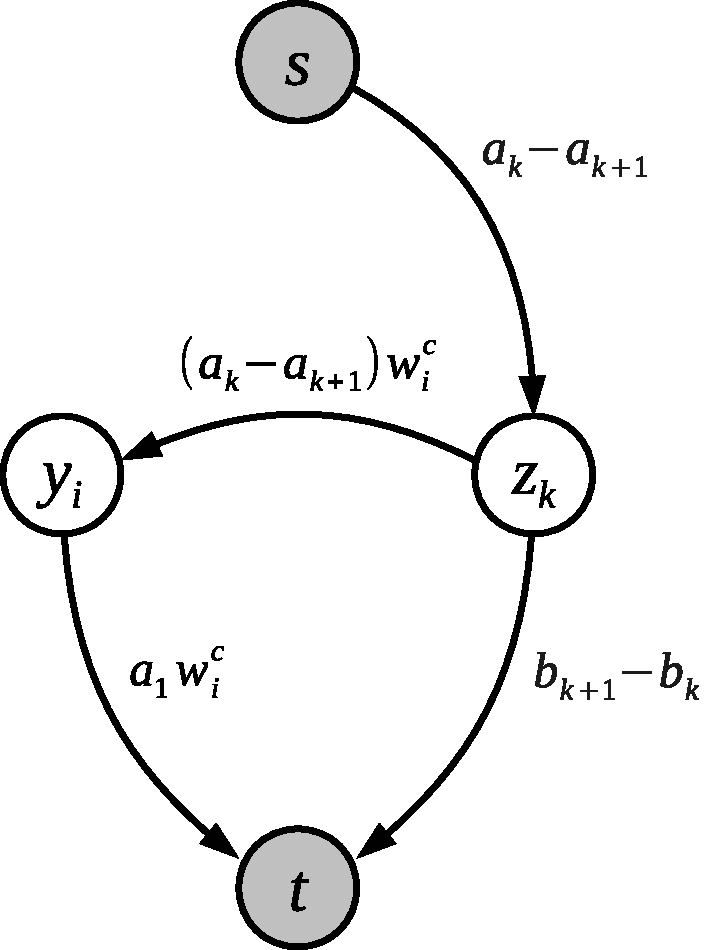
\includegraphics[width=0.45\columnwidth]{Methodology/figures/stmincut}&
                                                                         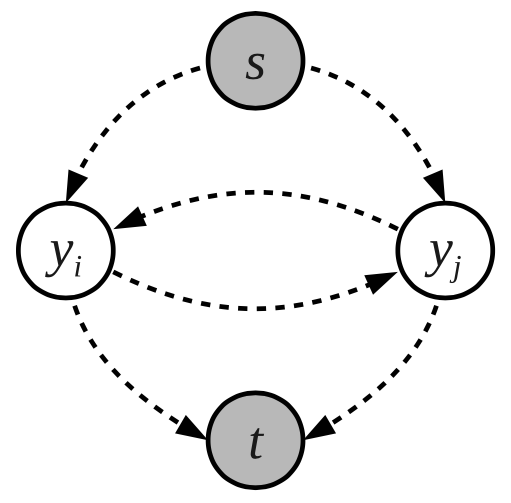
\includegraphics[width=0.5\columnwidth]{Methodology/figures/unary_pairwise.png}\\
                                                                         {\small (a)} & {\small (b)} 
  \end{tabular}
  \caption{\label{fig:stmincut} $st$-graph
    construction~\cite{gouldlearning} for
    equation~\eqref{eqn:posiform}, unary and pairwise terms.
    Every cut corresponds to an assignment to the random
    variables, where variables associated with nodes in the
    ${\cal S}$ set take the value one, and those associated with
    nodes in the $\T$ set take the value zero. With slight abuse
    of notation, we use the variables to denote nodes in our
    graph.}
\end{figure}

\begin{align}
  \label{eq:z_consecutive_constraint}
  z_{k+1} \leq z_k
\end{align}

\noindent this property give rise to further development of
parameter vector~\eqref{eq:llsvm_param} and feature
vector~\eqref{eq:llsvm_feature} which are used in latent
structural SVM.

In order to construct the \emph{st-min-cut} graph,
\citename{gouldlearning} rewrote
equation~\eqref{eqn:binary_concave_z} into
\emph{posiform}~\cite{Boros:MATH02}:

\begin{align}
  \label{eqn:posiform}  
  E^c(\by_c, \bz)
  &= b_1 - (a_1 - a_K) + \sum_{i \in c} a_1 w^c_i y_i
  {}+ \sum_{k = 1}^{K - 1} \left( b_{k+1} - b_k \right) z_k\\
  &+ \sum_{k = 1}^{K - 1} \left( a_k - a_{k+1} \right) \bar{z}_k
  {}+ \sum_{k = 1}^{K - 1} \sum_{i \in c} \left( a_k - a_{k+1}
    \right) w^c_i \bar{y}_i z_k \nonumber
\end{align}

\noindent where $\bar{z}_k = 1 - z_k$ and $\bar{y}_i = 1 - y_i$.
$a_1$ is assumed to be greater than $0$ so that all coefficients
are positive (recall we assume $b_1=0$ in section~\ref{sec:llep}
and we have $a_k > a_{k+1}$ and $b_k < b_{k+1}$). After proving
\emph{submodularity} of the energy function~\eqref{eqn:posiform},
\citename{gouldlearning} constructed the \emph{st-min-cut} graph
based on equation~\eqref{eqn:posiform}.

The construction is explained in \figref{fig:stmincut}. Figure
(a) denotes construction for equation~\eqref{eqn:posiform}. For
each lower linear envelope potential edges are added as follows:
for each $i \in c$, add an edge from $y_i$ to $t$ with weight
$a_1 w^c_i$; for each $i \in c$ and $k = 1, \ldots, K-1$, add an
edge from $z_k$ to $y_i$ with weight $(a_{k} - a_{k+1}) w^c_i$;
and for $k = 1, \ldots, K-1$, add an edge from $s$ to $z_k$ with
weight $a_k - a_{k+1}$ and edge from $z_k$ to $t$ with weight
$b_{k+1} - b_k$. Figure (b) denotes construction for unary and
pairwise terms (see \cite{Kolmogorov:PAMI04}). For unary edges (4
edges on both sides), weights on each edge are corresponding to
values in input unary terms accordingly. For pairwise edges (2
edges in the middle), both edges share the same weight which
equals to the input pairwise term.

\section{Learning the Lower Linear Envelope with Latent Information}
\label{sec:learning}

With the inference algorithm in hand, we now can develop the
learning algorithm for weighted lower linear envelope potentials
using the latent structural SVM framework. We begin by
transforming the equation~\eqref{eqn:binary_concave_z} into a
linear combination of parameter vector and feature vector. Then a
two-step algorithm was developed to solve the latent structural
SVM.


\subsection{Transforming Between Representations}
\label{sec:latent_linEnv_represent}

The latent structural SVM formulation (see
equation~\eqref{eq:latent_ssvm_linearcomb}) requires that the
energy function be expressed as a linear combination of features
and weights while our higher-order potential is represented as
the minimum over a set of linear functions. However,
in~\ref{sec:exact_inference} we reformulated the piesewise linear
functions into a quadratic pseudo-Boolean
function~\eqref{eqn:binary_concave_z} by introducing auxiliary
variables. Now we show function~\eqref{eqn:binary_concave_z}
itself is an inner product of parameter vector and feature vector
with latent information. We first noticed that the function can
be expanded as a summation of $2K-1$ terms:

\begin{align}
  \label{eq:originalenergy}
  E^c(y_c,z)&=a_1W_c(y_c)+b_1+\sum_{k=1}^{K-1}z_k((a_{k+1}-a_k)W_c(y_c)+b_{k+1}-b_k)\nonumber\\ 
            &=a_1W_c(y_c)+\sum_{k=1}^{K-1}(a_{k+1}-a_k)z_kW_c(y_c)+\sum_{k=1}^{K-1}(b_{k+1}-b_k)z_k
\end{align}

Here we use the fact of equation~\eqref{eq:shift_invariant} and
let $b_1=0$. Now we can reparameterize the energy function
as
\begin{align}
  \label{eq:llsvm_innerprod_energy}
  E^c(\by_c,\bz; \btheta) = \btheta^T \! \phi(\by_c,\bz)
\end{align}

\noindent where:

\begin{equation}
\label{eq:llsvm_param}
  \theta_k = \left\{
    \begin{aligned}
      & a_1	& \text{for} \ k=1\\
      & a_k-a_{k-1} & \text{for}\ 1< k \leq K\\
      & b_{k+1-K}-b_{k-K} & \text{for} \ K<k\le2K-1\\
    \end{aligned}
  \right.
\end{equation}

\begin{equation}
\label{eq:llsvm_feature}
  \phi_k = \left\{
		\begin{aligned}
      & W_c(\by_c) 	& \text{for} \ k=1\\
      & W_c(\by_c)\bz_k & \text{for}\ 1<k\le K\\
      & \bz_k & \text{for} \ K<k\le2K-1\\
		\end{aligned}
  \right.
\end{equation}

Under this formulation, inference
problems~\eqref{eq:latentssvm_full_inf}
and~\eqref{eq:latentssvm_latent_inf} introduced in
section~\ref{sec:latent-struct-svms} can be written as:

\begin{align}
  \label{eq:linenv_full_inf}
  (\mathbf{\hat{y}}_k(\btheta),\mathbf{\hat{z}}_k(\theta))=\argmin_{(\mathbf{y}
  \times \mathbf{z}) \in \mathcal{Y} \times \mathcal{Z}}
  \btheta^T\cdot\phi(\mathbf{y}_k,\mathbf{z}_k)
\end{align}
and
\begin{align}
  \label{eq:linenv_latent_inf}
  \mathbf{z}^*_k(\btheta) = \argmin_{\mathbf{z} \in \mathcal{Z}}
  \btheta^T \cdot \phi(\mathbf{y}_k,\mathbf{z}_k)
\end{align}

There are 2 facts worth to mention. The first fact is
that in our previous construction of minimum-$st$-cut graph the
latent variable $\bz$ is already included. Therefore, we can
apply our inference algorithm directly on our 2 new formulations.

However, for equation~\eqref{eq:linenv_latent_inf} there exists
more efficient algorithm. At training stage the ground-truth
labels $y_i$ is a function input thus completely observed.
Therefore, the term $((a_{k+1}-a_k)W_c(\by_c)+b_{k+1}-b_k)$ in
equation~\ref{eq:originalenergy} becomes constant. So we can
infer latent variable $\bz$ explicitly by:
\begin{align}
  \label{eq:linenv_effi_infer_latent}
  z_k^c &=
          \begin{cases}
            0 & \text{if $((a_{k+1}-a_k)W_c(y_c)+b_{k+1}-b_k)\geq0$} \\
            1 & \text{otherwise}.
          \end{cases}
\end{align}

\begin{figure}[t]
  \centering
  \includegraphics[width=0.8\columnwidth]{Methodology/figures/linEnvLatentFig.png}
  \caption{\label{fig:concave} Example piecewise-linear concave
    function of $W_{\!c}(\by_c) = \sum_{i \in c} w^c_i y_i$.
    Assume the second linear function is active namely
    $\bz^c=(1,1,0,0)$. The result of linear combination of
    parameter vector and feature vector is same as quadratic
    psuedo-Boolean function.}
\end{figure}

To show the equivalence between
equation~\eqref{eqn:binary_concave_z} and
equation~\eqref{eq:llsvm_innerprod_energy} we consider the
example illustrated in figure~\ref{fig:concave}. Assume the
inferred latent vector $\bz^c=(1,1,0,0)$. Plug it into
equation~\eqref{eq:llsvm_feature} the energy function can be
written as:
\begin{align*}
  E^c(\by_c,\bz; \btheta) &=
  \begin{bmatrix}
    a_1\\
    a_2-a_1\\
    a_3-a_2\\
    a_4-a_3\\
    b_2\\
    b_3-b_2\\
    b_4-b_3
  \end{bmatrix}^T
  \begin{bmatrix}
    W_c(\by_c) \\
    W_c(\by_c) \\
    0\\
    0\\
    1\\
    0\\
    0
  \end{bmatrix}\\
  &=a_1W_c(\by_c)+(a_2-a_1)W_c(\by_c)+b_2\\
  &=a_2W_c(\by_c)+b_2
\end{align*}

Therefore, assignments inferred by graph-cut algorithm can be
directly encoded into a linear combination by using our latent
structural SVM formulation for learning purpose. The remaining
task is to ensure the concavity of $\btheta$. We do this by
adding the following constraint:

\begin{align}
  A\btheta\geq0 \text{,\;~~~} A=
                  \begin{bmatrix}
                    1 & \mathbf{0} & \mathbf{0}\\
                    \mathbf{0} & -\mathbf{1} & \mathbf{0}\\
                    \mathbf{0} & \mathbf{0} & \mathbf{P}
                  \end{bmatrix}\in \mathbb{R}^{(2K-1)\times(2K-1)}
\end{align}

\noindent where $-\mathbf{1}$ is a matrix of size $(K-1)\times(K-1)$ and
$\mathbf{P}$ is an identity matrix of size $(K-1)\times(K-1)$.

One subtle problem we found during experiments is that the
algorithm can be stuck small numerical value. To avoid this we
add small slack variables $\epsilon$ on those constraints:

\begin{align}
  \label{eq:concave_constraint}
  A\btheta\geq\epsilon \text{,\;~~~} A=
                  \begin{bmatrix}
                    1 & \mathbf{0} & \mathbf{0}\\
                    \mathbf{0} & -\mathbf{1} & \mathbf{0}\\
                    \mathbf{0} & \mathbf{0} & \mathbf{P}
                  \end{bmatrix}\in \mathbb{R}^{(2K-1)\times(2K-1)}
\end{align}

\noindent where $\epsilon$ usually equal to $\mathbf{1}^{-15}$ in our
experiments.

\subsection{Latent Structural SVM Learning}
\label{sec:mrflssvm_learning_algo}

With the inner product formulation
(equation~\eqref{eq:llsvm_innerprod_energy}) of higher order
energy function in hand, we now able to develop our latent
structural SVM learning algorithm. The energy function (higher
order function together with unary and pairwise functions) can be
written as:
\begin{equation}
  E_{all}(y,z) = \begin{bmatrix}
    \btheta^H\\
    \theta^{unary}\\
    \theta^{pairwise}
  \end{bmatrix}^T 
  \cdot \begin{bmatrix}
    \phi^H\\
    \phi^{unary}\\
    \phi^{pairwise}
  \end{bmatrix}=\theta_{all}^T\cdot\phi_{all}
\end{equation}
where $\btheta^H\in \real$ is the parameter vector in higher
order equation~\eqref{eq:llsvm_innerprod_energy} of size $2K-1$.
$\theta^{unary}$ and $\theta^{pairwise}$ are both scalars.
$\phi^\textrm{unary} = \sum_i \psi^U_i\!(y_i)$ and
$\phi^\textrm{pairwise} = \sum_{ij} \psi^P_{ij}(y_i, y_j)$.
Therefore, the size of $\theta_{all}$ is $2K+1$.

Plug equation~\eqref{eq:linenv_full_inf} and
equation~\eqref{eq:linenv_latent_inf} into object
function~\eqref{eq:latent_ssvm_object}, the latent structural SVM
object function for our problem can be derived as a difference of
two convex functions:

\begin{align}
\label{eq:lssvm_object}
  \min_\theta\bigg(\frac{1}{2}\|\theta\|^2+
  C\sum_{i=1}^{n}\big(\max_{(\mathbf{\hat{y}} \times
  \mathbf{\hat{z}}) \in \mathcal{Y} \times \mathcal{Z}}
  [\theta\cdot\phi(\mathbf{\hat{y}},\mathbf{\hat{z}}) +
  \Delta(\mathbf{y}_i,\mathbf{\hat{y}},\mathbf{\hat{z}})]\big)\bigg)\\
  -C\sum_{i=1}^{n}\big(\max_{\mathbf{z} \in \mathcal{Z}} \theta \cdot
  \phi(\mathbf{y}_i,\mathbf{z})\big)\nonumber
\end{align}

As mentioned by \citename{yu2009learning} the Concave-Convex
Procedure (CCCP)~\cite{yuille2002concave} can be used to solve the
optimization problem. Our algorithm contains two stages. We first
imputes the latent variables $\bz$ explicitly by
equation~\eqref{eq:linenv_latent_inf}. Namely solving the
``latent variable completion'' problem~\cite{yu2009learning}:

\begin{align}
  \bz_i^*=\argmax_{\mathbf{z} \in \mathcal{Z}} \theta \cdot
  \phi(\mathbf{y}_i,\mathbf{z})
\end{align}

The inference result $z_i^*$ for $i=1,\dots,n$ is used as
completely observed for later stage. With the latent variable
$z_i^*$ which best explains the ground-truth data $y_i$ in hand,
updating the parameter vector $\btheta$ is similar to solve the
standard max-margin optimization problem described
in~\cite{gouldlearning}:

\begin{align}
\label{eq:mrflssvm_object}
  \min_\theta\bigg(\frac{1}{2}\|\theta\|^2+
  C\sum_{i=1}^{n}\big(\max_{(\mathbf{\hat{y}} \times
  \mathbf{\hat{z}}) \in \mathcal{Y} \times \mathcal{Z}}
  [\theta\cdot\phi(\mathbf{\hat{y}},\mathbf{\hat{z}}) +
  \Delta(\mathbf{y}_i,\mathbf{\hat{y}},\mathbf{\hat{z}})]\big)\bigg)\\
  -C\sum_{i=1}^{n}\big(\theta \cdot
  \phi(\mathbf{y}_i,\mathbf{z}_i^*)\big) \nonumber
\end{align}

The last problem remaining is the initialization method. Because
our objective function~\eqref{eq:mrflssvm_object} is not convex
and the CCCP algorithm is only guaranteed to converge to a local
minimum or saddle point\cite{yuille2002concave}, initialization
of $\btheta$ might affect the performance of our algorithm. Since
there are no theoretical solution for this problem, we only
propose an empirical \algref{alg:init_theta}:

\begin{algorithm}[ht]
  \begin{algorithmic}[1]
    \STATE{$gap=\frac{1}{K}$, $a_1=\U(0,1e6)$, $b_1=0$,
      $sp_1=(0,0)$, $w_0=0$, $counter=2$} \FOR{each
      clique $c\in \C$} \STATE{Compute weighted clique value
      $w_c=W_c(y_C)$} \IF{$w_c-w_{c-1}>gap$}
    \STATE{$upbound = a_{counter}w_c+b_{counter}$\\
      $sp_{counter}=(w_c,\U(upbound-0.5,upbound))$\\
      Calculate $a_{counter}$ and $b_{counter}$ using
      $sp_{counter-1}$ and $sp_{counter}$\\
      $counter=counter+1$}
    \ENDIF
    \ENDFOR
    \STATE{If $counter<K$, remaining $a$s and $b$s are all set to
      be $a_{counter}$ and $b_{counter}$} \STATE{Calculate
      $\btheta$ using $\{a_k,b_k\}_{k=1}^K$}
  \end{algorithmic}
  \caption{\label{alg:init_theta} Empirical initialization
    algorithm for $\btheta$}
\end{algorithm}

We assume that the more evenly distributed of $W_c(Y_c)$ where
$c\in\C$ on $x$ axis, the more rich representation (number of
linear functions) the energy function should have. In order to
initialize $\btheta$, we first determine the x-coordinate of
sampled points $sp$. Then we sample its y-coordinate from a
uniform distribution $\U(upbound,upbound-0.5)$ to add some
randomness in our initialization as well as maintain concavity.
Linear parameters $a_k$ and $b_k$ are later calculated using
those sampled points $sp_k$ and $sp_{k-1}$. At last we encode
$\{a_k,b_k\}_{k=1}^K$ into $\btheta$ using
equation~\eqref{eq:llsvm_param}.

Our optimization algorithm is summarized in
\algref{alg:learning}.

\begin{algorithm}[hb]
  \begin{algorithmic}[1]
    \STATE{Set $MaxIter = 100$}
    \STATE{ {\bf input} training set $\{\by_i\}_{i=1}^{n}$, regularization constant $C > 0$,
      and tolerance $\epsilon \geq 0$}
    \STATE{Initialize $\btheta$ using \algref{alg:init_theta}}
    \REPEAT
    \STATE{Set $iter = 0$}
    \FOR{each training example, $i = 1, \ldots, n$}
    \STATE{compute $ \bz_i^*=\argmax_{\mathbf{z} \in \mathcal{Z}}
      \theta \cdot \phi(\mathbf{y}_i,\mathbf{z}) $}
    \ENDFOR

    \STATE{ {\bf initialize} active constraints set $\C_i = \{ \}$ for all $i$}
    \REPEAT

    \STATE{solve the quadratic programming problem in
      equation~\ref{eq:mrflssvm_object} with respect to active
      constraints set $\C_i$ for all $i$ and concavity constraints
      $A\btheta\geq \epsilon$ to get
      $\hat{\btheta}$ and $\hat{\bxi}$}

    \FOR{each training example, $i = 1, \ldots, n$}
    \STATE{compute $\hat{\by_i},\hat{\bz_i} = \argmin_{\by}
      E(\by,\bz; \hat{\btheta}) - \Delta(\by, \bz, \by_i)$}
    \IF{$\hat{\xi}_i + \epsilon \!<\! \Delta(\hat{\by_i},
      \hat{\bz_i}, \by_i) -
      E(\hat{\by_i},\hat{\bz_i}; \hat{\btheta}) + E(\by_i, \bz_i^*; \hat{\btheta})$}
    \STATE{$\C_i \leftarrow \C_i \cup \{\by_i^\star\}$}
    \ENDIF
    \ENDFOR
    \UNTIL{no more violated constraints}
    \STATE{ {\bf return} parameters $\hat{\btheta}$}
    \STATE{Set $iter = iter+1$}

    \UNTIL{$iter\geq MaxIter$}
    \STATE{ {\bf return} parameters $\hat{\btheta}$}
  \end{algorithmic}
  \caption{\label{alg:learning} Learning lower linear envelope
    MRFs with latent variables.}
\end{algorithm}



\clearpage
\cleardoublepage


%%% Local Variables:
%%% mode: latex
%%% TeX-master: "../thesis"
%%% End:

%%
%% Template Experiments.tex
%%

\chapter{Experiments}
\label{cha:Experiments}

In this chapter, we follow our previous approach
in~\cite{gouldlearning} and conduct two experiments with
different purposes. We first examine our method's effectiveness
by comparing our results with~\cite{gouldlearning,Gould:ICML2011}
on a synthetic checkerboard. We then extend our work to the
real-world ``GrabCut'' problem introduced in
section~\ref{sec:grabcut} and comparing our result with previous
researches \cite{Rother:SIGGRAPH04} to investigate
our new methods' performance.

\section{Synthetic Checkerboard}
\label{sec:synth-check}

Since the main contribution of our work is extending our previous
approximate formulation of lower linear envelope potentials to an
exactly formulation, it is necessary to compare the results on
synthetic checkerboard to previous work~\cite{gouldlearning}.

In this section we will experiment our method on three different
problem instances: checkerboard with squares containing
monotonous color~\ref{sec:monot-color-squar}, checkerboard with
squares containing more pixels of one color over
another~\ref{sec:unbal-color-squar} and checkerboard with
uniformly colored squares containing unbalanced
color~\ref{sec:unif-distr-squar}.

\subsection{Experiment Settings}
\label{sec:experiment-settings}

An image of synthetic checkerboard contains $8 \times 8$ pixel
squares. Each square (clique) contains $16 \times 16$ (256)
pixels. The color of each pixel is either black $0$ or white $1$.
Given a ground-truth checkerboard image
$\by^*=y^*_1,\dots,y^*_{16384}$, the observed unary terms
$\by=y_1,\dots,y_{16384}$ are generated as followings. Let
$\eta_0$ and $\eta_1$ be the signal-to-noise ratios for the black
and white squares, the unary terms are generated by destroying
groud-truth label to noisy input
\begin{align}
  \label{eq:noisy_checkerboard}
  y_i = \eta_0 \ind{y^\star_i = 0} - \eta_1 \ind{y^\star_i = 1} + \delta_i
\end{align}
where $\delta_i
\sim \U(-1, 1)$ is additive i.i.d.\ uniform noise. $\ind{x}$ is
an indicator function which equals $1$ when $x$ is true and $0$
otherwise. The task is to recover the ground-truth checkerboard
from the noisy input.

Our MRF is constructed on this image by associating each node in
the MRF to each pixel in the image. Thus our MRF contains $8
\times 8 \times 256 = 16,384$ variables. The energy function used
in this experiment follows equation~\eqref{eq:energyfunction_UPH}
without pairwise terms.

\begin{align}
  \label{eq:syncheck_energy}
  E(\by;\btheta)=\theta^U\sum_{i\in \N}{\phi^U(\by_i)}+
  \sum_{\by_c\in \C}{\phi^H(\by_c,\bz_c;\btheta^H)}
\end{align}
where $\phi^U(\by_i)=\by_i$ and $\theta^U$ is a scalar weight for
unary terms. $\phi^H(\by_c,\bz_c;\btheta^H)=\btheta^{H\;T} \!
\phi(\by_c,\bz_c)$ is equivalent to
equation~\eqref{eq:llsvm_innerprod_energy} and added for each
square (clique $c$) in the checkerboard. The number of linear
equations $K$ in equation~\eqref{eq:llsvm_param} is set to be
$10$. The parameters $\theta^U$ and $\btheta^H$ are learned using
\algref{alg:learning} with $MaxIter=100$. 

\subsection{Monotonous Colored Squares}
\label{sec:monot-color-squar}

\begin{figure}[hb]
  \centering
  \setlength{\tabcolsep}{2pt}
  \begin{tabular}{cc}
    \includegraphics[width=0.5\columnwidth]{Experiments/figures/mono_gt.png}&
                                                                            \includegraphics[width=0.5\columnwidth]{Experiments/figures/mono_noisy.png}\\
    {\small (a)} & {\small (b)} 
  \end{tabular}
  \caption{\label{fig:mono_checkerboard} Example for monotonous
    colored squares. figure (a) is the ground-truth checkerboard.
    Figure (b) is the noisy input (unary terms) destroyed by
    equation~\eqref{eq:noisy_checkerboard}}
\end{figure}

We first repeat our previous black and white checkerboard
experiment~\cite{Gould:ICML2011,gouldlearning} in order to
examine the correctness of our new formulation. Each clique
(square) $c\in \C$ in the checkerboard contains either all white
pixels $y_i=1 ,\;\forall i \in c$ or all black pixels $y_i=0
,\;\forall i \in c$. Figure~\ref{fig:mono_checkerboard}
illustrates the ground-truth checkerboard and the noisy input
destroyed by equation~\eqref{eq:noisy_checkerboard} with
$\eta_0=\eta_1=0.1$. Figure~\ref{fig:mono_results} shows the
results of our new method (on the bottom) together with our
previous method~\cite{gouldlearning} (on the top).

\begin{figure}[ht]
  \centering
  \setlength{\tabcolsep}{2pt}
  \begin{tabular}{cc}
    \includegraphics[width=0.3\columnwidth]{Experiments/figures/mono_gt.png}&
                                                                              \includegraphics[width=0.4\columnwidth]{Experiments/figures/mono_old.png}\\
    {\small (a)} & {\small (b)} \\
    \includegraphics[width=0.3\columnwidth]{Experiments/figures/mono_gt.png}&
                                                                              \includegraphics[width=0.4\columnwidth]{Experiments/figures/mono_new.png}\\
    {\small (c)} & {\small (d)} 
  \end{tabular}
  \caption{\label{fig:mono_results} Results comparison for
    monotonous colored squares. Figure (a) and Figure (c) are
    inferred checkerboard from our previous and current
    formulation separately. Figure (b) and Figure (d) are lower
    linear envelopes learned by each formulation.}
\end{figure}

From figure~\ref{fig:mono_results} we conclude that both
formulations can recover checkerboard perfectly so our new
formulation's accuracy is as good as previous one. However,
there are significant differences between structural SVM
formulation (previous method) and latent structural SVM
formulation. There are $10$ active linear functions in
figure~\ref{fig:mono_results} (b) while there are only $2$ active
linear functions in figure~\ref{fig:mono_results} (d). Shapes
learned by each formulation are also significantly different.

In general, the second result is more preferable than the first
one. The reason is despite the image contains 64 cliques, there
are only two kinds of squares in the image: completely black and
completely white. Accordingly, our model only see two kinds of
cliques: completely $0$s (black) and completely $1$s (white). In
this case, a lower linear envelope contains two linear functions
is enough for encoding consistency information. This is reflected
in figure~\ref{fig:mono_results} (d) which gives least penalty
(0) when the clique value $W_C(y_c)$ equals either $0$ or $1$. It
gives the highest penalty when $W_C(y_c)$ is in the middle
because our model has least probability seen that in training
data. The results certificates that our latent structural SVM
formulation can learn lower linear envelope exactly. Therefore,
we say that our new method learns more preferable lower linear
envelope.

In terms of computational performance, because our initial point
are generated randomly using \algref{alg:init_theta}, the
performance various between runnings. On average it takes 2
\emph{outer loops} and 47 \emph{inner loops} to converge. Which
means the latent structural SVM formulation spends $3.5$ times
iterations to converge than previous one ($27$ iterations).
Each \emph{inner loop} took under 1s with inference taking about
120ms on a $2.7$GHz dual-core Intel CPU, which is the same as our
previous method.



\subsection{Unbalanced Colored Squares}
\label{sec:unbal-color-squar}

Experiment in section~\ref{sec:monot-color-squar} proves that our
latent structural SVM formulation can learn the lower linear
envelope exactly. In this section we conduct further experiment
to investigate its capability of representing unbalanced input.
The desirable result of this experiment should be the shape of
the lower linear envelope shifting along with the changing of
input data.

We design our checkerboards contain unbalanced colored squares as
shown in figure~\ref{fig:unba_checkerboard}.

\begin{figure}[hb]
  \centering
  \setlength{\tabcolsep}{2pt}
  \begin{tabular}{cc}
    \includegraphics[width=0.5\columnwidth]{Experiments/figures/unba_black.png}&
                                                                            \includegraphics[width=0.5\columnwidth]{Experiments/figures/unba_white.png}\\
    {\small (a)} & {\small (b)} 
  \end{tabular}
  \caption{\label{fig:unba_checkerboard} Example for unbalanced
    colored squares. In figure (a) $75\%$ cliques contain more
    than $85\%$ black pixels while $25\%$ cliques contain more
    than $85\%$ white pixels. Figure (b) is the opposite of
    figure (a)}
\end{figure}

As before, figure~\ref{fig:unba_results} shows results learned by
structural SVM (top row) and latent structural SVM (bottom row).
The accuracy performance of both methods are almost the same.
Both methods are able to recover $45\%-50\%$ pixels. The shape of
each formulations' results are both preferable and very similar
when compared to each other. The most significant difference is
the number of linear functions (10 active linear functions v.s.
2). In terms of computational performance, our previous method
only takes $10$ iterations to converge while the latent
structural SVM formulation takes $89$ iterations. Our new method
is much more computational expensive than our previous method.

\begin{figure}[ht]
  \centering
  \setlength{\tabcolsep}{2pt}
  \begin{tabular}{cc}
    \includegraphics[width=0.5\columnwidth]{Experiments/figures/unba_black_res_old.png}&
                                                                              \includegraphics[width=0.5\columnwidth]{Experiments/figures/unba_white_res_old.png}\\
    {\small (a)} & {\small (b)} \\
    \includegraphics[width=0.5\columnwidth]{Experiments/figures/unba_black_res_new.png}&
                                                                              \includegraphics[width=0.5\columnwidth]{Experiments/figures/unba_white_res_new.png}\\
    {\small (c)} & {\small (d)} 
  \end{tabular}
  \caption{\label{fig:unba_results} Results comparison for
    unbalanced colored squares. Figure (a) and Figure (b) are
    lower linear (more black and more white) envelopes learned by
    structural SVM. Figure (c) and Figure (d) are learned by
    latent structural SVM.}
\end{figure}

\bigskip
\bigskip
\bigskip
\bigskip
\bigskip
\bigskip

\subsection{Uniformly Colored Squares}
\label{sec:unif-distr-squar}

All of the above experiments show that our new method can
significantly simplify the shape of the lower linear envelope
function while maintaining the inference performance at the same
level. However, one significant cost is the computational
performance. It still remains obscure if there exists any other
advantages. In this section we design a much harder problem.
$W_c(y_c)$ is uniformly distributed from $0$ to $1$.
Figure~\ref{fig:ba_gt} shows the result. The preferable shape of
the lower linear envelope should contain a line which is parallel
to the x-axis.

\begin{figure}[t]
  \centering
  \includegraphics[width=0.5\columnwidth]{Experiments/figures/ba_gt.png}
  \caption{\label{fig:ba_gt} Uniformly colored squares example.
    $W_{\!c}(\by_c) = \sum_{i \in c} w^c_i y_i$ is uniformly
    distributed from $0$ to $1$.}
\end{figure}

Results are shown in figure~\ref{fig:ba_res}. As we can see
that shapes are very different between two formulations. Our
latent structural formulation (figure~\ref{fig:ba_res} (b))
learned a very flat representation of the lower linear envelope
function, which is much preferable, while the structural SVM
formulation preserves much concavity in the shape. This might
because in previous work~\cite{gouldlearning,Gould:ICML2011}
we imposed strict concave constraints on parameter vector
$\btheta$.

The performance of accuracy also various significantly. Under
this formulation our new method is still able to recover
$45\%-50\%$ pixels while our previous can only recover
$25\%-30\%$ pixels on average. Therefore, our new formulation
finally outperforms previous one. In terms of computational
performance, the new formulation takes $129$ \emph{inner loops}
in total (2 \emph{outer loops}) while our previous formulation
takes $75$ iterations to converge. Although the new formulation
is still more computational expensive than previous one, the gap
decreases significantly.

We consider all of those improvements are due to our new method
is able to learn the lower linear envelope exactly.

One subtle thing is that the linear function on the right side in
figure~\ref{fig:ba_res} (b) decreases sharply which seems
abnormally at first glance. The reason is that we assume $b_1=0$
in section~\ref{sec:llep} which fixes the y-intercept of the
first linear function to be zero. Therefore the last linear
function can be arbitrarily deep while the first linear function
is fixed at the original point.

\clearpage

\begin{figure}[ht]
  \centering
  \setlength{\tabcolsep}{2pt}
  \begin{tabular}{cc}
    \includegraphics[width=0.5\columnwidth]{Experiments/figures/ba_res_old.png}&
                                                                            \includegraphics[width=0.55\columnwidth]{Experiments/figures/ba_res_new.png}\\
    {\small (a)} & {\small (b)} 
  \end{tabular}
  \caption{\label{fig:ba_res} Results of uniformly colored
    squares experiment. Figure (a) is the result learned by
    structural SVM formulation. Figure (b) is the result learned
    by latent structural SVM formulation.}
\end{figure}

\subsection{Conclusions}
\label{sec:synth-check-conc}

From above experiments we conclude our findings as followings:

\begin{itemize}
\item All of those experiments verified that our latent
  structural formulation is able learn the lower linear envelope
  exactly.
\item In general (see section~\ref{sec:monot-color-squar} and
  section~\ref{sec:unbal-color-squar}), our new method have
  equivalent accuracy performance to our old method (structural
  SVM formulation\cite{Gould:ICML2011,gouldlearning}).
\item In terms of computational performance, the new formulation
  is much more computational expensive than the previous one
  during training. However, it is more efficient during testing
  due to it simplicity for the lower linear envelope potentials.
\item For harder problem (see
  section~\ref{sec:unif-distr-squar}), the new method outperforms
  the previous one significantly. The gap of computational
  performance also decreases a significant amount.
\end{itemize}

\clearpage

\section{Foreground Extraction}
\label{sec:foregr-extr}

To evaluate our method on real-world applications, we repeat the
``Interactive Figure-Ground Segmentation'' experiment in our
previous researches~\cite{gouldlearning,Gould:ICML2011}. As
described in section~\ref{sec:grabcut}, the goal of this
experiment is to extract foreground pixels from a bounding box of
the object. We follow settings in previous work and replace
the max margin algorithm with latent structural SVM
\algref{alg:learning}.

\subsection{Experiment Settings}
\label{sec:experiment-settings-grabcut}

The data set we use is collected by~\citename{Lempitsky:ICCV09}
which contains $50$ images (contains $630\times480$ pixels on
average) with ground-truth labels and user-annotated bounding
boxes. Following previous work we perform
\algref{alg:learning} by leave-one-out cross-validation on this
data set. In order to be comparable with previous results, the
performance is measured by \emph{accuracy}. Our energy function
for this problem is defined as:

\begin{align}
  \label{eq:grabcut_mrflssvm_energy}
  E(\by;\btheta)=\theta^U\sum_{i\in \N}{\phi^U(\by_i)}+
  \theta^P\sum_{(i,j)\in \E}{\phi^P(\by_i,\by_j)}+
  \sum_{\by_c\in \C}{\phi^H(\by_c,\bz_c;\btheta^H)}
\end{align}

As we described in section~\ref{sec:grabcut}, unary terms are
generated by GMMs (both foreground and background) trained by
\emph{GrabCut}~\cite{Rother:SIGGRAPH04} algorithm. The unary
terms are assigned as following:

\begin{table}[h]
  \normalsize
  \centering
  \begin{tabular}{|l|c|c|}
    \hline
    {\sc Unary} & {\sc $0$} & {\sc $1$}\\
    \hline
    $\phi^U(y_i)$ & $\phi^U(0,\bk_i,\btheta,\bz_i)$ & $\phi^U(1,\bk_i,\btheta,\bz_i)$ \\
    \hline
  \end{tabular}
  \caption{\label{tab:grabCut_unary} Table of GrabCut unary
    terms. $\phi^U$ is taken from
    equation~\eqref{eq:grabcut_energy}. $1$ is the label for
    foreground and $0$ for background}
\end{table}

The pairwise terms are defined as:
\begin{align}
  \label{eq:mrflssvm_grabcut_pairwise}
  \phi^P(\by_i,\by_j) = \frac{\lambda}{d_{ij}}[[y_i\neq y_j]]exp\bigg\{-\frac{||x_i-x_j||^2}{2\beta}\bigg\} \text{~,~for~~} \forall (i,j)\in \E
\end{align}

where $\E$ denotes the set of pairs of neighboring pixels which
is defined as 8-way adjacent pixels (horizontally, vertically and
diagonally). $d_{ij}$ is the Euclidean distance of neighboring
pixels. $x_i$ is the RGB value vector. $\beta$ denotes the
expectation over $(x_i-x_j)^2$. The only free parameter $\lambda$
is learned by \algref{alg:learning} during cross-validation and
determines the strength of the pairwise smoothness term.

The \emph{SLIC} algorithm introduced in
section~\ref{sec:superpixel} is used to generate cliques $c\in\C$
for higher order terms.
$\phi^H(\by_c,\bz_c;\btheta^H)=\btheta^{H\;T} \!
\phi(\by_c,\bz_c)$ is equivalent to
equation~\eqref{eq:llsvm_innerprod_energy} and added for each
clique $c$ in the image. The number of linear equations $K$ in
equation~\eqref{eq:llsvm_param} is set to be $10$.

Then we run the \algref{alg:learning} with $MaxIter=100$. Results
are shown in section~\ref{sec:grabcut_exp_result}. 

\subsection{Experiment Result}
\label{sec:grabcut_exp_result}

In this section we compare our new latent structural SVM
formulation's results with our previous
work~\cite{gouldlearning}. On average it takes $5.3$ hours to
train a cross-validation fold while our previous method only
takes $3$ hours. For some folds our method can take more than $8$
hours and still not converge. Table~\ref{tab:grabCut_acc} shows
comparison between different models:

\begin{table}[h]
  \normalsize
  \centering
  \begin{tabular}{|l|c|}
    \hline
    {\sc Model} & {\sc Accuracy}\\
    \hline
    Baseline & 90.9 \\
    \hline
    Structural SVM Formulation & 91.6 \\
    Latent SSVM Formulation & 92.27 \\
    \hline
  \end{tabular}
  \caption{\label{tab:grabCut_acc} GrabCut experiment results
    comparison. Data of Baseline model and Structural SVM model
    is from previous work~\cite{gouldlearning}.}
\end{table}

It turns out that our new formulation slightly outperforms our
previous method by $0.6\%$. The following
table~\ref{tab:grabCut_hist} shows a more detailed accuracy
distribution among $50$ images:

\begin{table}[h]
  \normalsize
  \centering
  \begin{tabular}{|l|c|}
    \hline
    {\sc Accuracy Interval} & {\sc Number of images}\\
    \hline
    Over $99.5\%$ & $35$ \\
    \hline
    $90\%-99.5\%$ & $9$ \\
    \hline
    $70\%-90\%$ & $4$ \\
    \hline
    $50\%-70\%$ & $1$ \\
    \hline
    Below $50\%$ & $1$ \\
    \hline
  \end{tabular}
  \caption{\label{tab:grabCut_hist} GrabCut results' accuracy
    distribution.}
\end{table}

From this table we can conclude that our new formulation performs
very well on $75\%$ of images in the data set. From
figure~\ref{fig:flower_results} to
figure~\ref{fig:portrait_results} show the comparison of results
which we illustrated in previous work~\cite{gouldlearning}.
Figure in the middle column is the ground-truth foreground image.
Figure on the left is the foreground inferred by our previous
method. Figure on the right is inferred by our new method.

% grabcut results

\begin{figure}[ht]
  \begin{center} \setlength{\tabcolsep}{0pt}
    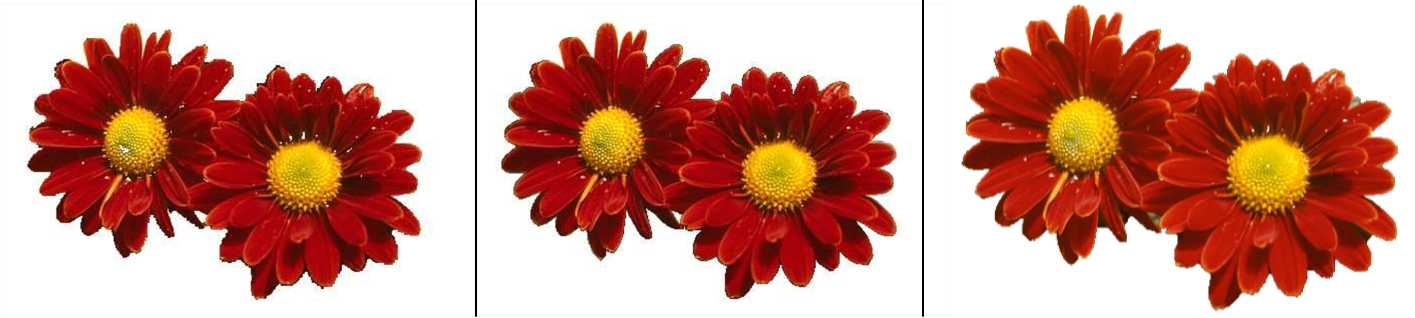
\includegraphics[width=\linewidth]{Experiments/figures/124080.png}
\\
  \caption{\label{fig:flower_results}GrabCut Results.}
  \end{center}
\end{figure}

\begin{figure}[ht]
  \begin{center} \setlength{\tabcolsep}{0pt}
    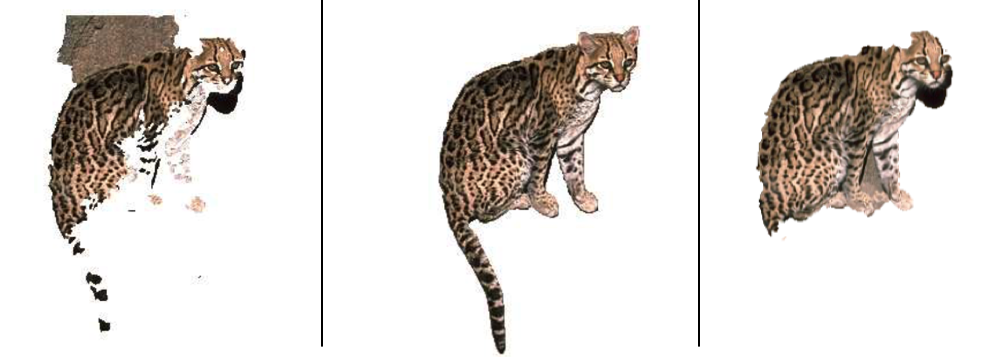
\includegraphics[width=\linewidth]{Experiments/figures/326038.png}
\\
  \caption{\label{fig:cheetah_results}GrabCut Results.}
  \end{center}
\end{figure}

\begin{figure}[ht]
  \begin{center} \setlength{\tabcolsep}{0pt}
    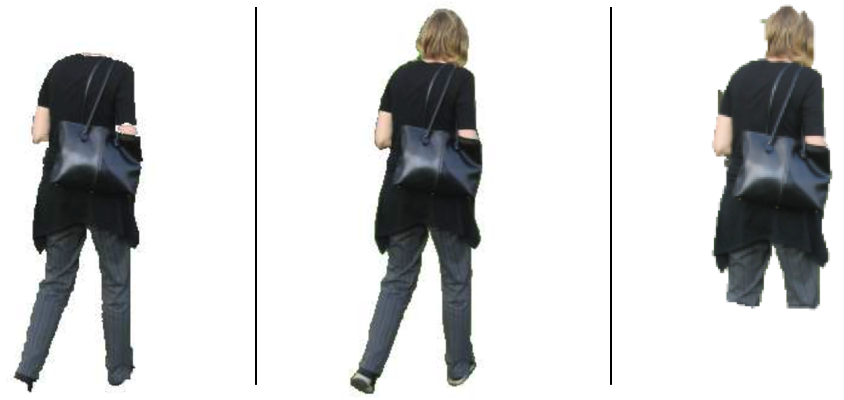
\includegraphics[width=\linewidth]{Experiments/figures/person5.png}\\
  \caption{\label{fig:person_results}GrabCut Results.}
  \end{center}
\end{figure}

In figure~\ref{fig:flower_results}, our new method has a very
strong results. It almost perfectly extracted the foreground
image. The accuracy is over $99.5\%$. In
figure~\ref{fig:cheetah_results} our new method still performs
better. However, it left the cheetah's tail out compared to our
previous method. One important thing to notice is that there are
many holes in the image on the left (inferred by our previous
method) while the image inferred by our new method is very smooth
without holes. This certificates that by learning the lower
linear envelope exactly, our new method has a better performance
on preserving higher order consistency. In
figure~\ref{fig:person_results} two methods have almost the same
performance. Previous method left the woman's head but was
able to capture her full legs while our new method only able to
capture half of her legs but with full head.

\bigskip
\bigskip
\bigskip
\bigskip

However, the performance various significantly between images. In
figure~\ref{fig:portrait_results}, even though the sculpture
inferred by our new method is still very smooth without any hole
on it, our method failed to segment the background out of the
foreground (there are large amount of pixels belong to stairs and
glass). Our model completely fails to learn the image
``189080.png'' which has the worst performance $42.5\%$ (the
\algref{alg:learning} stopped at the maximum number of iterations
which is 10 \emph{outer loops} and 100 \emph{inner loops} for
each \emph{outer loop}). The inferred foreground image is
completely blank as shown in figure~\ref{fig:grabcut_worst}.


\begin{figure}[t]
  \begin{center} \setlength{\tabcolsep}{0pt}
    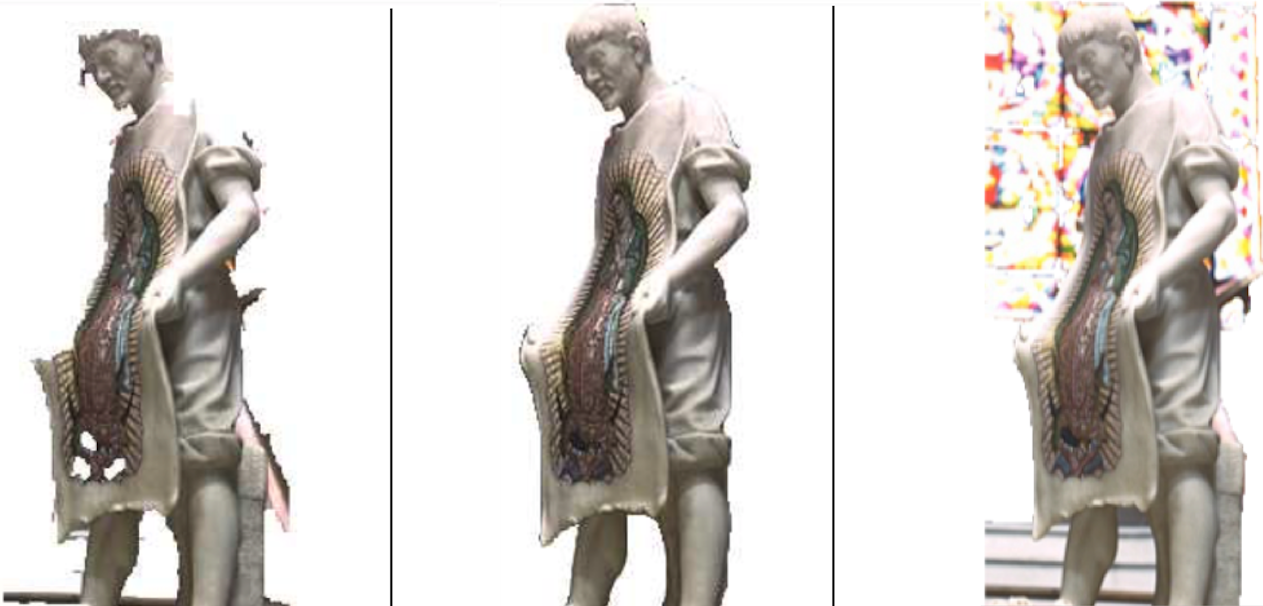
\includegraphics[width=\linewidth]{Experiments/figures/24077.png}\\
  \caption{\label{fig:portrait_results} GrabCut Results.}
  \end{center}
\end{figure}

\begin{figure}[t]
  \begin{center} \setlength{\tabcolsep}{0pt}
    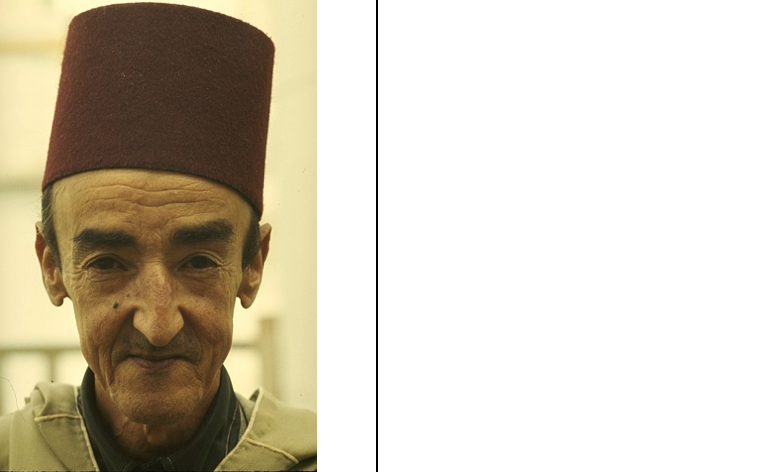
\includegraphics[width=0.5\linewidth]{Experiments/figures/189080.png}
\\
\caption{\label{fig:grabcut_worst} Worst accuracy image. The
  accuracy is only $42.5\%$. The foreground inferred is
  completely blank which means information learned by our model
  is failed to be generalize to this image.}
  \end{center}
\end{figure}

\clearpage

\subsection{Conclusions}
\label{sec:grabcut-conc}

From above experiments we conclude our findings as followings:

\begin{itemize}
\item In general, our new method outperforms previous one.
  The accuracy is increased by $0.6\%$. This might because our
  new method learns the lower linear envelope exactly thus has a
  richer representation than previous one.
\item In general, our new method has a better higher-order
  consistency. This can be seen from
  figure~\ref{fig:flower_results} to
  figure~\ref{fig:portrait_results}. This is also because the
  lower linear envelope function has better quality than our
  previous method.
\item The new method's performance various differently among
  images. The performance ranges from $42.5\%$ to $99.5\%$.
\item The new method is more computationally expensive than our
  previous method during training. It takes $5.3$ hours to train
  one cross-validation fold while previous method only takes
  $3$ hours. However, it is more efficient during testing due to
  it simplicity for the lower linear envelope potentials.
\item There seems like to exist some generalization issues in our
  \algref{alg:learning}. For example, the new method has bad
  performance of filtering background in
  figure~\ref{fig:portrait_results} and it completely fails to
  infer the figure~\ref{fig:grabcut_worst}.
\end{itemize}



\clearpage
\cleardoublepage



%%% Local Variables:
%%% mode: latex
%%% TeX-master: "../thesis"
%%% End:

%% 
%% 
%% 

\chapter{Modeling Higer-order Structural Dependencies with Markov Random Fields (MRFs)}
\chaptermark{MRF-LSSVMs}
\label{cha:mrf}

One challenging task in machine learning is recognizing and
labeling over complex and structured objects. Many applications,
such as image segmentation, motif finding and noun-phrase
parsing, involves representing jointly correlated sub-objects and
exploiting structural dependencies to identify higher level
objects. These objects usually have structural dependencies on
sub-objects (smaller components), \eg the human face has a strong
structural dependency on five sensory organs. The Markov Random
Fields (MRFs, are also called undirected Probabilistic Graphical
Models~\cite{bishop:2006:PRML}), is one of the most popular
framework in modeling structural dependencies. In this Chapter,
we propose novel exact inference and learning algorithms, the
MRF-LSSVMs (Latent Structural Support Vector Machine) framework,
to exploit MRFs' capabilities in modeling higher-order (more than
three entities) structural dependencies. The application of
MRF-LSSVMs to capture higher-order dynamics on time series is
discussed in \Chapref{cha:mrf_lssvm_app}.

Markov Random Fields (MRFs) are undirected Probabilistic
Graphical Models (PGMs). The formulation of MRFs is simply a
regularized joint probability distribution. One specialty of MRFs
is that they are factorized (conditional independent) over
\textbf{maximal cliques} (more details in~\Secref{sec:MRF}) of
random variables defined on the undirected
graph~\cite{bishop:2006:PRML}. In many applications, structural
information, such as sub-objects to the whole object
relationships and relationships between sub-objects, can be well
represented in maximal cliques. By defining each maximal clique's
probability distribution and optimizing over them, MRFs provide a
powerful framework for modeling complex higher-order
dependencies between entities.

Utilizing MRFs usually involves three steps: 1) designing energy
functions (un-normalized probability distribution) according to
the actual problem, 2) solving inference problem (MAP or energy
minimization), and 3) learning parameters from data set. With
respect to energy functions, our work focuses on Lower Linear
Envelope Potentials (LLEP), a class of higher-order potentials
defined as a concave piecewise linear function over a clique of
random variables. LLEP has been raising much interest in the
image segmentation area, in which the raw image input is used as
PGM's graph and pixels are treated as random variables. Maximal
cliques of the input image are usually detected at preprocessing
stage by using clustering algorithms such as
superpixel~\cite{achanta2012slic}. Success of LLEP on encoding
consistent constraints over large subsets of pixels in image
segmentation tasks has been witnessed in many
literatures~\cite{Kohli:CVPR07,Nowozin:2011, Song2015}. In this
chapter we focus on proposing a novel exact inference algorithm
for LLEP and design a learning algorithm under the LLSVM
framework. In \Chapref{cha:mrf_lssvm_app}, we will generalize the
MRF-LLSVMs framework into encoding consistent constraints among
time-series' entities.

In the second step, in order to solve the inference problem of
LLEP, \citename{kohli2009robust} proposed a method to represent a
class of higher order potentials with lower (upper) linear
envelope potentials. By introducing auxiliary
variables~\cite{Kohli:CVPR10}, they reduced the linear
representation to a pairwise form and proposed an approximate
algorithm with standard linear programming methods. However, they
only show an exact inference algorithm on at most three terms.
Following their approach, \citename{gouldlearning} extended their
method to a weighted lower linear envelope with arbitrary many
terms solved with an efficient algorithm. They showed that the by
introducing auxiliary variables into LLEP, a quadratic
pseudo-Boolean form~\cite{Boros:MATH02} can be developed. This
psuedo-Boolean form is submodular and can be inferred efficiently
and exactly through graph-cuts like
algorithms~\cite{Boykov:ICCV01}. However, in order to employ
Structural Support Vector Machine (SSVM) to solve the learning
problem of LLEP, \citename{gouldlearning} have to sample the LLEP
using a set of fixed space points. Althought this formulation can
be globally optimized by using the SSVM framework, it lost a rich
class of representations of energy function due to the fixed
space sampling. In this chapter, we an alternative formulation to
learn LLEP exactly. We introduce auxiliary variables back to LLEP
and propose a graph-cuts algorithm to infer observed variables
and auxiliary variables simultaneously. Experiments in
~\Secref{sec:synth-check} also show that LLEP under this
formulation the algorithm can be learned exactly from various
different probability distribution configurations.

The third and last difficulty is to design a learning algorithm
for our LLEP formulation. In previous work,
\citename{gouldlearning} sampled the LLEP with fixed space points
and solved the learning problem under the Structural Support
Vector Machine (SSVM) framework \cite{tsochantaridis2005large}.
However, since we add auxiliary variables back, SSVM does not fit
our case anymore. One of our main contribution is that we prove
that auxiliary variables introduced in LLEP can be formulated as
latent variables in SSVM. With additional convex constraints
added to the SSVM object, our formulation results to the Latent
SSVM (LSSVM) framework \cite{yu2009learning}. The LSSVM was
developed by \citename{felzenszwalb2008discriminatively} and
\citename{yu2009learning} independently in different ways. The
main idea is introducing a latent variable to extend the feature
vector, which results in an arbitrary loss function, e.g. Hinge
Loss, with an upper bound. Then the optimization was done by
using Concave-Convex Procedure (CCCP) algorithm, which is
guaranteed to decrease the objective function to a local minimum.
In this thesis, we propose a variant formulation of
\cite{gouldlearning} by rewriting the lower linear envelope
function directly into a linear combination with latent feature
vectors and developing the learning algorithm using the LSSVM.

The rest of the thesis is structured as follows:
\Secref{sec:RelatedWorks} introduces background and related works
of MRFs and LSSVM. \Secref{sec:inference} proposes our first
contribution, the exact inference method of LLEP with auxiliary
variables. In~\Secref{sec:learning}, we reformulate the LLEP into
a linear combination and develop the learning algorithm under the
LSSVM framework. \Secref{sec:synth-check} conduct experiments on
a synthetic checkerboard image to show the effectiveness of our
novel MRF-LLSVMs framework. Application of MRF-LLSVMs on real
financial time-series data set is discussed in
\Chapref{cha:mrf_lssvm_app}.

\section{Background \& Related Works}
\label{sec:RelatedWorks}

\subsection{Markov Random Fields}
\label{sec:MRF}
From a PGMs view (\figref{fig:prml_mrf}) \cite{Bishop:2007},
MRFs' joint probability distribution can be represented as an
undirected graph and each random variable can be represented as a
node in the graph. A \textbf{clique} is a fully connected subset
of nodes: there exists a path between any pair of nodes in it. A
\textbf{maximal clique} is a clique such that it is not possible
to include any other nodes from the graph in the set without it
ceasing to be a clique.
\begin{figure}[ht]
  \centering
  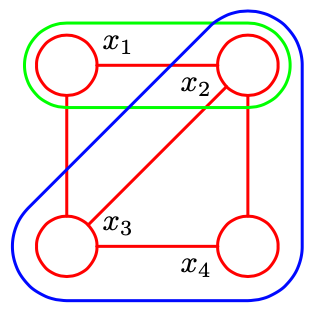
\includegraphics[width=0.3\columnwidth]{Part2/figures/prml_mrf}
  \caption{\label{fig:prml_mrf} An example PGM of MRFs. Each node
    in this graph corresponds to a random variable in this PGM's
    joint probability distribution. A clique is outlined in green
    circle and a maximal clique is outlined in blue circle.}
\end{figure}
Let $C$ denotes a maximal clique in one graph and $\vy_C$ denotes
the set of variables in that clique. Then the joint distribution
can be written as:
\begin{align}
  p(\vy)=\frac{1}{Z}\prod_{C}{\Psi_C(\vy_C)}
\end{align}
\noindent where $\Psi$ is called \emph{potential functions} which
can be defined as any non-negative functions and
$Z=\sum_{\vy}\prod_{C}{\Psi_C(\vy_C)}$ which is a normalization
constant. To infer labels which best explains input data set, we
can find the \emph{maximum a posteriori} (MAP) labels by solving
$\vy^*=\argmax_{\vy}p(\vy)$. However, potential functions are
restricted to be non-negative to ensure it is a probability
distribution.

In order to have more flexible representations of probability
distributions, by taking exponential of potential terms, MRFs can
be represented as a regularized joint log-probability
distribution of arbitrary non-negative functions over a set of
maximal cliques on the PGM graph~\cite{bishop:2006:PRML}. Thus
the joint distribution becomes:
\begin{align}
  p(\vy)=\frac{1}{Z}exp(-\sum_{C}{E_C(\vy_C)})
\end{align}
\noindent where $E$ is called \emph{energy functions} which can be
arbitrary functions. Therefore, \emph{maximum a posteriori}
problem is equivalent to \emph{energy minimization} problem,
which is also known as the \emph{inference} problem:
\begin{align}
  \vy^*=\argmax_{\vy}p(\vy)=\argmin_{\vy}(\sum_{C}{E_C(\vy_C)})
\end{align}

The \emph{inference} problem is computationally expensive. There
has been many sub-optimal algorithms such as max-product
algorithm \cite{Globerson:NIPS07} been proposed to solve the
general MRFs' inference problem. However, \citename{Boros:MATH02}
proved that for submodular energy functions, there exist
efficient algorithms based on graph cuts
\cite{Ishikawa:CVPR09,Kohli:TR08} and are guaranteed to converge
to the global optimum. In \Secref{sec:inference} we formulate the
MRFs with Lower Linear Envelope Potentials (LLEP) as
psuedo-boolean functions and devise a graph cut algorithm for
exact inference.

As for the \emph{learning} problem, conventionally, energy
functions can be decomposed into three weighted parts: nodes
$\gN$, edges $\gE$ and higher order cliques (any group which has
more than 3 fully connected nodes in it)
$\gC$~\cite{Szummer:ECCV08}. Each term has its own weights. Let
$\vw$ be the vector of parameters and $\phi$ be arbitrary feature
function, then the energy can be decomposed as a set linear
combinations of weights and feature vectors:

\begin{align}
  \label{eq:energyfunction_UPH}
  E(\vy;\vw)=\sum_{i\in \gN}{\vw_i^U\phi^U(\vy_i)}+
  \sum_{(i,j)\in \gE}{\vw_{ij}^P\phi^P(\vy_i,\vy_j)}+
  \sum_{\vy_C\in \gC}{\vw_C^H\phi^H(\vy_C)}
\end{align}

\noindent where $U$ denotes \emph{unary} terms, $P$ denotes
\emph{pairwise} terms and $H$ denotes \emph{higher order} terms
(when $|C|>2$ namely each clique contains more than two
variables).

A weight vector $\vw$ is more preferable if it gives the
ground-truth assignments $\vy_t$ less than or equal to energy
value than any other assignments $y$:

\begin{align}
E(y_t,w)\leq E(y,w)~ \text{,~}\forall y \neq y_t
\text{,~} y\in \sY
\end{align}

Thus the goal of \emph{learning} MRFs is to learn the parameter
vector $\vw^*$ which returns the lowest energy value for the
ground-truth labels $y_t$ relative to any other assignments
$y$~\cite{Szummer:ECCV08}:

\begin{align}
\vw^* = argmax_{\vw}(E(y_t,w)-E(y,w))~ \text{,~}\forall y \neq y_t
\text{,~} y\in \sY
\end{align}

Solving the learning problem of MRFs is also computationally
expensive. In this thesis, we employ the efficient Latent
Structural Support Vector Machines (LSSVMs) algorithm to solve
our MRFs.

\subsection{Latent Structural SVMs}
\label{sec:latent-struct-svms}

The Structural Support Vector Machines (SSVMs) (also called
max-margin
framework)~\cite{Taskar:ICML05,tsochantaridis2005large} is a
principled approach to learn weights of pairwise MRFs
\citename{Szummer:ECCV08,Gould:ICML2011}.
\citename{gouldlearning} extended this framework with additional
linear constraints to enforce concavity on the weights, thus
allowing them to be used to learn MRFs with lower linear envelope
potentials. However, because SSVM does not include latent
variables in its feature vector, such methods only approximately
learn higher-order functions. In this thesis, we propose an
algorithm to optimize the energy function exactly by introducing
auxiliary variables back into the feature vector and solving the
learning problem using the Latent Structural SVMs (LSSVMs)
framework~\cite{yu2009learning}. To include unobserved
information, \citename{yu2009learning} extended the joint feature
function in structural SVM with latent variables and re-wrote the
objective function of SSVM into a difference of two convex
functions. This formulation can be solved using the
Concave-Convex Procedure (CCCP)\cite{yuille2002concave} which is
two-stages algorithm that guarantee to convergence to a local
minimum.

Specifically, given an a linear combination of features vector
$\phi(\vx ,\vy) \in \sR^m$ and weights $\vtheta \in \sR^m$, and a
set of $n$ training examples $\{\vy_i\}_{i=1}^n$ max-margin
framework can be used to solve optimized solution $\vtheta^*$. To
include unobserved information in the model,
Yu\cite{yu2009learning} extended the joint feature
function\cite{tsochantaridis2005large} $\phi(\vx,\vy) $ with a
latent variable $\vh\in \mathcal{H}$ to $\phi(\vx,\vy,\vh) $. So
the inference problem becomes
\begin{align}
  \label{eq:latent_ssvm_linearcomb}
  f_\theta(x) = \argmax_{(\vy \times \vh) \in \sY
  \times \sH} \vtheta\cdot\phi(\vx,\vy,\vh)
\end{align}

Accordingly, the loss function can be extended as

$$
\Delta((\vy_i,\vh^*_i(\theta)),(\hat{\vy}_i(\vtheta),\hat{\vh}_i(\vtheta)))
$$

\noindent where

\begin{align}
  \label{eq:latentssvm_full_inf}
 (\hat{\vy}_i(\vtheta),\hat{\vh}_i(\vtheta))=\argmax_{(\vy
  \times \vh) \in \mathcal{Y} \times \mathcal{H}}
\theta\cdot\phi(\vx_i,\vy,\vh)
\end{align}

\begin{align}
  \label{eq:latentssvm_latent_inf}
  \vh^*_i(\theta) = \argmax_{\vh \in \mathcal{H}} \theta \cdot
  \phi(\vx_i,\vy_i,\vh)
\end{align}

The loss function under this formulation measures difference
between the inferred result pair $(\hat{\vy}_i(\theta),
\hat{\vh}_i(\theta))$ and the pair $(\vy_i(\theta),
\vh_i^*(\theta))$ which best explains the training data. However,
under this formulation the ``loss augmented inference'' used in
structural SVMs\cite{tsochantaridis2005large} to remove the
complexity cannot be performed due to the dependence of loss
function $\Delta$ on hidden variables $\vh^*_i(\theta)$.
\citename{yu2009learning} argued that in real world applications
hidden variables are usually intermediate results and are not
required as an output\cite{yu2009learning}. Therefore, the loss
function can only focus on the inferenced hidden variables
$\hat{\vh}_i(\theta)$ which leads to:

$$
\Delta((\vy_i,\vh^*_i(\theta)),(\hat{\vy}_i(\theta),\hat{\vh}_i(\theta)))
=
\Delta(\vy_i,\hat{\vy}_i(\theta),\hat{\vh}_i(\theta))
$$

Thus the upper bound used in standard structural
SVMs\cite{tsochantaridis2005large} can be extended to:

\begin{align}
  \nonumber\Delta((\vy_i,\vh^*_i(\theta)),(\hat{\vy}_i(\theta),\hat{\vh}_i(\theta)))
  &\leq \bigg(\max_{(\hat{\vy} \times \hat{\vh}) \in
    \mathcal{Y} \times \mathcal{H}}
    [\theta\cdot\Psi(\vx_i,\hat{\vy},\hat{\vh}) +
    \Delta(\vy_i,\hat{\vy},\hat{\vh})]\bigg)\\
  &-\max_{\vh \in \mathcal{H}} \theta \cdot
    \Psi(\vx_i,\vy_i,\vh)
\end{align}

Hence the optimization problem for Structural SVMs with latent
variables becomes

\begin{align}
\label{eq:latent_ssvm_object}
  \min_\theta\bigg(\frac{1}{2}\|\theta\|^2+
  C\sum_{i=1}^{n}\big(\max_{(\hat{\vy} \times
  \hat{\vh}) \in \mathcal{Y} \times \mathcal{H}}
  [\theta\cdot\Psi(\vx_i,\hat{\vy},\hat{\vh}) +
  \Delta(\vy_i,\hat{\vy},\hat{\vh})]\big)\bigg)\\
  -C\sum_{i=1}^{n}\big(\max_{\vh \in \mathcal{H}} \theta \cdot
  \Psi(\vx_i,\vy_i,\vh)\big)\nonumber
\end{align}

\noindent which is a difference of two convex functions. Problem
of this formulation can be solved using the Concave-Convex
Procedure (CCCP)\cite{yuille2002concave} which is guaranteed to
converge to a local minimum. \citename{yu2009learning} proposed a
two stages algorithm. In the first step the latent variable
$\vh_i^*$ which best explains training pair $(\vx_i, \vy_i)$ is
found by solving equation~\eqref{eq:latentssvm_latent_inf}. This
step is also called the ``latent variable completion'' problem.
In the second step $\vh_i^*$ is used as completely observed to
substitute $\vh$ in equation~\eqref{eq:latent_ssvm_object}.
Therefore, solving equation~\eqref{eq:latent_ssvm_object} is
equivalent to solve the standard structural SVM problem.

In contrast to SVM, the latent structural SVM only provides an
optimization framework and cannot be directly applied. In order
to use it, the inference algorithm, as well as the MRF feature
function, loss function, and latent variable completion
problem~\cite{yu2009learning} must first be specified. Our
implementation of these terms are described in
section~\ref{sec:opt}.

\section[MRFs with LLEPs]{Markov Random Fields (MRFs) with Lower
  Linear Envelope Potentials (LLEPs)}
\label{sec:inference}

Energy functions can be decomposed over nodes $\gN$, edges $\gE$
and higher order cliques $\cal C$~\cite{Szummer:ECCV08}. Let
$\vw$ be vector of parameters and $\psi$ be arbitrary feature
function, then the energy can be decomposed as a set of linear
combinations of weights and feature vectors:

\begin{align}
  \label{eq:energyfunction_UPH}
  E(\vy;\vw)&=\sum_{i\in \gN}{\vw_i^U\psi^U(\vy_i)}+ \notag\\
  & \sum_{(i,j)\in \gE}{\vw_{ij}^P\psi^P(\vy_i,\vy_j)}+
  \sum_{\vy_C\in \cal C}{\vw_C^H\psi^H(\vy_C)}
\end{align}

\noindent where $U$ denotes \emph{unary} terms, $P$ denotes
\emph{pairwise} terms, $H$ denotes \emph{higher order} terms. In
this section we mainly focus on one class of higher-order
potentials $\psi^H$ defined as a concave piecewise linear
function which is known as \emph{Lower Linear Envelope
  Potentials} (LLEP). 

LLEP has been studied extensively in Markov Random Fields area
for encouraging consistency over large
cliques~\cite{Kohli:CVPR07,Nowozin:2011,Gould:ICML2011}. In
\Secref{sec:llep}, we begin with developing standard Markov
Random Fields (MRFs) (equation~\eqref{eq:energyfunction_UPH})
with the LLEP as energy functions. We then show how to perform
exact inference under this formulation in
\Secref{sec:exact_inference}. The optimization algorithm for our
formulation will be discussed in \Secref{sec:learning}.

\subsection{Higher-order Energy Functions: Weighted Lower Linear
  Envelope Potentials (LLEP)}
\label{sec:llep}

Let $\cal C$ denotes the set of all maximal cliques
and $\vy_c=\{y_i |\text{\,for\,} i \in C_j\}$ denotes set of
binary random variables where $y_i\in \{0,1\}$ in clique $C_j$, a
weighted lower linear envelope potential over $\vy_c$ is defined
as the minimum over a set of $K$ linear functions as:
%
\begin{align}
  \psi^H_c\!(\vy_c) \, &= \min_{k=1, \ldots, K} \left\{ a_k W_{\!c}(\vy_c) + b_k \right\}.
  \label{eqn:potential2}
\end{align}
%
where $W_{\!c}(\vy_c) = \sum_{i \in c} w_i^c y_i$ with $w^c_i
\geq 0$ and $\sum_{i \in c} w^c_i = 1$ which are weights for each
clique. $(a_k, b_k) \in \sR^2$ are the linear function
parameters. We illustrate an example with four linear functions
in \figref{fig:concave}.

\begin{figure}[t]
  \centering
  \includegraphics[width=0.8\columnwidth]{Part2/figures/linEnvLatentFig.png}
  \caption{\label{fig:concave} Example piecewise-linear concave
    function of $W_{\!c}(\vy_c) = \sum_{i \in c} w^c_i y_i$.
    Assume the second linear function is active namely
    $\vz^c=(1,1,0,0)$ (equation \ref{eqn:binary_concave_z}). The result of linear combination of
    parameter vector and feature vector is same as quadratic
    pseudo-Boolean function.}
\end{figure}

% % to_replace
% \begin{figure}[ht]
%   \centering
%   \includegraphics[width=0.6\columnwidth]{Part2/figures/not_redundant}
%   \caption{\label{fig:nonredundant} Example lower linear envelope
%     $\psi^H_c\!(\by_c)$ (shown solid) with three terms (dashed).
%     When $W_{\!c}(\by_c) \leq W_1$ the first linear function is
%     active, when $W_1 < W_{\!c}(\by_c) \leq W_2$ the second
%     linear function is active, otherwise the third linear
%     function is active.}
% \end{figure}

Inference on energy function contains lower linear potentials is
the same as the standard equation~\eqref{eq:energyfunction_UPH}
and is given by:
\begin{align}
  \label{eq:min_energy}
  \vy^* = \argmin\energy{\vy}
\end{align}

Suppose that parameters $\{(a_k, b_k)\}_{k=1}^K$ are sorted in
decreasing order of $a_k$. From \emph{Definition 3.1}
\cite{gouldlearning} we know that the $k$-th linear function is
said to be \emph{active} if there exists $x \in (0, 1)$ such that
the following two inequalities hold
\begin{align}
  a_{k-1} x + b_{k-1} &> a_k x + b_k \nonumber \\
  a_{k+1} x + b_{k+1} &> a_k x + b_k
  \label{eqn:nonred_in_ab}
\end{align}
%
The $k$-th linear function is said to be \emph{redundant}
(\emph{Definition 3.2}~\cite{gouldlearning}) if it is not active
for any assignment to $\vy_c$ in any clique $c \in \gC$ or is only
active whenever another linear function is also active.
Figure \ref{fig:redundant} depicts such conditions. As a
result, removing redundant functions from the potential does not
chang the energy function.


From section~\ref{sec:MRF} we have already introduced that an
\emph{energy function} may contain \emph{unary}, \emph{pairwise}
and \emph{higher-order} potentials (see
equation~\eqref{eq:energyfunction_UPH}). In this section we
mainly focus on one class of higher-order potentials $\phi^H$
defined as a concave piecewise linear function which is known as
\emph{lower linear envelope potentials}. This has been studied
extensively in Markov Random Fields area for encouraging
consistency over large
cliques~\cite{Kohli:CVPR07,Nowozin:2011,Gould:ICML2011}.

Let $\gC$ denotes the set of all maximal cliques in an image and
$\vy_c=\{y_i |\text{\,for\,} i \in c\}$ denotes set of random
variables in the clique $c$, a weighted lower linear envelope
potential~\cite{gouldlearning} over $\vy_c$ is defined as the
minimum over a set of $K$ linear functions as:
%
\begin{align}
  \psi^H_c\!(\vy_c) \, &= \min_{k=1, \ldots, K} \left\{ a_k W_{\!c}(\vy_c) + b_k \right\}.
  \label{eqn:potential2}
\end{align}
%
where $W_{\!c}(\vy_c) = \sum_{i \in c} w_i y_i$ with $w^c_i \geq
0$ and $\sum_{i \in c} w^c_i = 1$ which are weights for each
clique. $(a_k, b_k) \in \sR^2$ are the linear function
parameters. We illustrate an example~\cite{gouldlearning} with
three linear functions in \figref{fig:nonredundant}.
%
\begin{figure}[ht]
  \centering
  \includegraphics[width=0.6\columnwidth]{Part2/figures/not_redundant}
  \caption{\label{fig:nonredundant} Example lower linear envelope
    $\psi^H_c\!(\vy_c)$ (shown solid) with three terms (dashed).
    When $W_{\!c}(\vy_c) \leq W_1$ the first linear function is
    active, when $W_1 < W_{\!c}(\vy_c) \leq W_2$ the second
    linear function is active, otherwise the third linear
    function is active.}
\end{figure}

Suppose that parameters $\{(a_k, b_k)\}_{k=1}^K$ are sorted in
decreasing order of $a_k$. \citename{gouldlearning} (Definition
3.1) defines that the $k$-th linear function is said to be
\emph{active} if there exists $x \in (0, 1)$ such that the
following two inequalities hold
\begin{align}
  a_{k-1} x + b_{k-1} &> a_k x + b_k \nonumber \\
  a_{k+1} x + b_{k+1} &> a_k x + b_k
  \label{eqn:nonred_in_ab}
\end{align}
%
The $k$-th linear function is said to be \emph{redundant}
(\emph{Definition 3.2}~\cite{gouldlearning}) if it is not active
for any assignment to $\vy_c$ in any clique $c \in \gC$ or is only
active whenever another linear function is also active.
Figure \ref{fig:redundant} depicts such conditions. As a
result, removing redundant functions from the potential does not
chang the energy function.

\begin{figure}[ht]
  \centering
  \includegraphics[width=1\columnwidth]{Part2/figures/redundant}
  \caption{\label{fig:redundant} Example lower linear envelope
    with redundant linear functions. On the left figure, the
    solid yellow line is always inactive. On the right figure,
    the solid purple line intersects $line \; 1$ and $line \; 2$
    at the red point. It's only active when $line \; 1$ and $line
    \; 2$ are both active. Both solid lines are redundant linear
    functions hence can be removed without changing their energy
    function.}
\end{figure}
%

To ensure potentials do not contain redundant linear functions
(functions that would never be active), \citename{gouldlearning}
proposed a constraint on parameters of the envelope. The $k$-th
linear function is not redundant if the following condition is
satisfied:
%
\begin{align}
    0
    <
    \frac{b_k - b_{k-1}}{a_{k-1} - a_k}
    <
    \frac{b_{k+1} - b_k}{a_k - a_{k+1}}
    <
    1.
  \label{eq:nonredundant}
\end{align}
%
Another important property of equation~\eqref{eq:min_energy} is
shift invariant (vertically). We write
$\widetilde{\psi}^{H}_c\!(\vy_c)$ by shift
equation~\eqref{eqn:potential2} vertically with an arbitrary
amount $b^{const}\in R$
$$\widetilde{\psi}^{H}_c\!(\vy_c) = \min_{k=1, \ldots, K}
\left\{a_k W_{\!c}(\vy_c) + b_k + b^\textrm{const} \right\}$$
%
Then we have
\begin{align}
  \argmin_{\vy_c} \psi^H_c\!(\vy_c)
  = \argmin_{\vy_c} \widetilde{\psi}^{H}_c\!(\vy_c).
  \label{eq:shift_invariant}
\end{align}
%
Therefore, in the following discussion without loss of generality
we assume $b_1 = 0$ thus $b_k\geq0 \text{\; for \;} k=1,\dots,n$.

\subsection{Exact Inference}
\label{sec:exact_inference}

Exact inference on MRFs has been extensively studied in past
years. Researchers found that, energy functions which can be
transformed into quadratic pseudo-Boolean
functions~\cite{Ishikawa:PAMI03,Ishikawa:CVPR09,Rother:CVPR09}
are able to be minimized exactly using \emph{graph-cuts} like
algorithms~\cite{Freedman:CVPR05,Hammer:1965} when they satisfy
submodularity condition~\cite{Boros:MATH02}.
\citename{Kohli:TR08} and \citename{Gould:ICML2011} adapted those
results to perform exact inference on lower linear envelope
potentials. In this section we mainly focus on describing the
minimum \emph{$st$-$cut$} graph constructed by
Gould~\cite{Gould:ICML2011,gouldlearning} for exact inference of
energy function (equation ~\eqref{eq:min_energy}) containing
lower linear envelope potentials.

Following the approach of \citename{Kohli:CVPR10},
\citename{Gould:ICML2011,gouldlearning} transformed the weighted
lower linear envelope potential in
equation~\eqref{eqn:potential2} into a quadratic pseudo-Boolean
function by introducing $K-1$ auxiliary variables $\vz =
\left(z_1, \ldots, z_{K-1}\right)$ with $z_k\in \{0,1\}$:

\begin{align}
  E^c(\vy_c, \vz) &= a_1 W_{\!c}(\vy_c) + b_1 \notag \\
  &+ \sum_{k = 1}^{K-1} z_k \left( \left(a_{k+1} - a_k\right) W_{\!c}(\vy_c) + b_{k+1} - b_k \right)
  \label{eqn:binary_concave_z}
\end{align}

\noindent for a single clique $c \in \cal C$. Under this
formulation, minimizing the pseudo-Boolean function over $\vz$ is
equivalent to selecting (one of) the active functions(s) from
equation~\eqref{eqn:potential2}. Another important property of
optimized $\vz$ under this formulation is that it automatically
satisfies the constraint
%
$$z_{k+1} \leq z_k$$
%
This property give rise to further development of parameter
vector and feature vector (equation~\eqref{eq:llsvm_param} and
~\eqref{eq:llsvm_feature}) which are used in latent structural
SVM. By introducing latent variables within the energy function,
we can learn richer energy representations than previous
study~\cite{gouldlearning} and solve inference problem exactly
within polynomial number of iterations.

In order to construct the minimum \emph{$st$-$cut$} graph, we
rewrite equation~\eqref{eqn:binary_concave_z} into
\emph{posiform}~\cite{Boros:MATH02}:

\begin{align}
  \label{eqn:posiform}  
  E^c(\vy_c, \vz)
  &= b_1 - (a_1 - a_K) + \sum_{i \in c} a_1 w^c_i y_i \notag\\
  & + \sum_{k = 1}^{K - 1} \left( b_{k+1} - b_k \right) z_k
    + \sum_{k = 1}^{K - 1} \left( a_k - a_{k+1} \right)
    \bar{z}_k\notag\\
  & + \sum_{k = 1}^{K - 1} \sum_{i \in c} \left( a_k - a_{k+1}
    \right) w^c_i \bar{y}_i z_k
\end{align}

\noindent where $\bar{z}_k = 1 - z_k$ and $\bar{y}_i = 1 - y_i$.
$a_1$ is assumed to be greater than $0$ so that all coefficients
are positive (recall we assume $b_1=0$ in section~\ref{sec:llep}
and we have $a_k > a_{k+1}$ and $b_k < b_{k+1}$). Since the energy function~\eqref{eqn:posiform}
is submodular, the \emph{st-min-cut} graph can be constructed 
based on equation~\eqref{eqn:posiform}.


\begin{figure}[t]
  \centering
  \setlength{\tabcolsep}{2pt}
  \begin{tabular}{cc}
    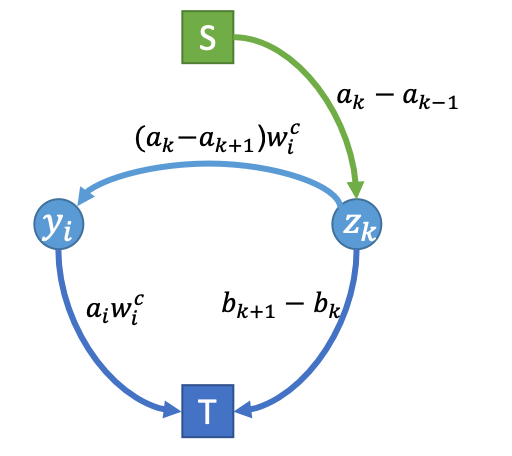
\includegraphics[width=0.47\columnwidth]{Part2/figures/ho.png}&
                                                                         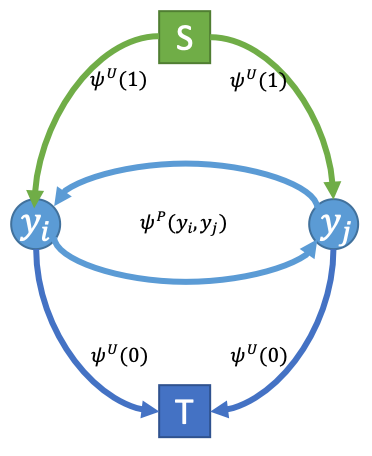
\includegraphics[width=0.37\columnwidth]{Part2/figures/up.png}\\
                                                                         {\small (a)} & {\small (b)} 
  \end{tabular}
  \caption{\label{fig:stmincut} $st$-graph construction for
    equation~\eqref{eqn:posiform}, unary and pairwise terms.
    Every cut corresponds to an assignment to the random
    variables, where variables associated with nodes in the $\gS$
    set take the value one, and those associated with nodes in
    the $\gT$ set take the value zero. With slight abuse of
    notation, we use the variables to denote nodes in our graph.}
\end{figure}


The construction (including unary and pairwise) is explained in
\Figref{fig:stmincut}. Figure (a) denotes construction for
equation~\eqref{eqn:posiform}. For each lower linear envelope
potential edges are added as follows: for each $i \in c$, add an
edge from $y_i$ to $t$ with weight $a_1 w^c_i$; for each $i \in
c$ and $k = 1, \ldots, K-1$, add an edge from $z_k$ to $y_i$ with
weight $(a_{k} - a_{k+1}) w^c_i$; and for $k = 1, \ldots, K-1$,
add an edge from $s$ to $z_k$ with weight $a_k - a_{k+1}$ and
edge from $z_k$ to $t$ with weight $b_{k+1} - b_k$. Figure (b)
denotes construction for unary and pairwise terms (see
\cite{Kolmogorov:PAMI04}). For unary edges (4 edges on both
sides), weights on each edge are corresponding to values in input
unary terms accordingly. For pairwise edges (2 edges in the
middle), both edges share the same weight which equals to the
input pairwise term.

\section[Solving MRFs under LSSVMs]{Solving MRFs under the Latent
  Structrual SVMs (LSSVM) Framework}
\label{sec:opt}

With the inference algorithm in hand, we now can develop the
learning algorithm for weighted lower linear envelope potentials
using the Latent Structural SVMs (LSSVMs) framework. In
\Secref{sec:learning}, we begin by transforming the
equation~\eqref{eqn:binary_concave_z} into a linear combination
of parameter vector and feature vector. A two-step algorithm was
developed to solve the latent structural SVM in
\Secref{sec:mrflssvm_learning_algo}.


\subsection{Transforming Between Representations}
\label{sec:learning}

The latent structural SVM formulation requires that the energy
function be formulated into a linear combination of features and
weights while our higher-order potential is represented as the
minimum over a set of linear functions. However,
in~\ref{sec:exact_inference} we reformulated the piesewise linear
functions into a quadratic pseudo-Boolean function in
equation~\eqref{eqn:binary_concave_z} by introducing auxiliary
variables. Now we show equation~\eqref{eqn:binary_concave_z}
itself is an inner product of parameter vector and feature vector
with latent information. Note that the function can be expanded
as a summation of $2K-1$ terms:

\begin{align}
  \label{eq:originalenergy}
  E^c(y_c,z)
  =&a_1W_c(y_c)+\sum_{k=1}^{K-1}(a_{k+1}-a_k)z_kW_c(y_c) \notag \\
   &+\sum_{k=1}^{K-1}(b_{k+1}-b_k)z_k
\end{align}

Here we use the fact of equation~\eqref{eq:shift_invariant} and
let $b_1=0$. Now we can reparameterize the energy function
as
\begin{align}
  \label{eq:llsvm_innerprod_energy}
  E^c(\vy_c,\vz; \vtheta^H) = \vtheta^{H^T} \! \psi^H(\vy_c,\vz)
\end{align}

\noindent where:

\begin{equation}
\label{eq:llsvm_param}
  \theta_k^H = \left\{
    \begin{aligned}
      & a_1	& \text{for} \ k=1\\
      & a_k-a_{k-1} & \text{for}\ 1< k \leq K\\
      & b_{k+1-K}-b_{k-K} & \text{for} \ K<k\le2K-1\\
    \end{aligned}
  \right.
\end{equation}

\begin{equation}
\label{eq:llsvm_feature}
  \psi_k^H = \left\{
		\begin{aligned}
      & W_c(\vy_c) 	& \text{for} \ k=1\\
      & W_c(\vy_c)\vz_k & \text{for}\ 1<k\le K\\
      & \vz_k & \text{for} \ K<k\le2K-1\\
		\end{aligned}
  \right.
\end{equation}

Under this formulation, similar to \cite{yu2009learning}, the inference problem
can be given by:

\begin{align}
  \label{eq:linenv_full_inf}
  (\mathbf{y}^*_k(\vtheta^H),\mathbf{z}^*_k(\theta^H))=\argmin_{(\mathbf{y}
  \times \mathbf{z}) \in \mathcal{Y} \times \mathcal{Z}}
  \vtheta^{H^T}\cdot\psi^H(\mathbf{y}_k,\mathbf{z}_k)
\end{align}
and
\begin{align}
  \label{eq:linenv_latent_inf}
  \mathbf{z}^*_k(\vtheta) = \argmin_{\mathbf{z} \in \mathcal{Z}}
  \vtheta^{H^T} \cdot \psi^H(\mathbf{y}_k,\mathbf{z}_k)
\end{align}

There are two facts worth to mention. The first fact is that in
our previous construction of minimum $st-cut$ graph the latent
variable $\vz$ is already included. Therefore, we can apply our
inference algorithm directly on our two new formulations. The
second fact is that for equation~\eqref{eq:linenv_latent_inf},
there exists a more efficient algorithm. At training stage, the
ground-truth labels $y_i$ is an input and is completely observed.
Therefore, the term $((a_{k+1}-a_k)W_c(\vy_c)+b_{k+1}-b_k)$ in
equation~\eqref{eq:originalenergy} becomes constant. So we can
infer latent variable $\vz$ explicitly by:
\begin{align}
  \label{eq:linenv_effi_infer_latent}
  z_k^c &=
          \begin{cases}
            0 & \text{if $((a_{k+1}-a_k)W_c(y_c)+b_{k+1}-b_k)\geq0$} \\
            1 & \text{otherwise}.
          \end{cases}
\end{align}

To show the equivalence between
equation~\eqref{eqn:binary_concave_z} and
equation~\eqref{eq:llsvm_innerprod_energy} we consider the
example illustrated in figure~\ref{fig:concave}. Assume the
inferred latent vector $\vz^c=(1,1,0,0)$. Plug it into
equation~\eqref{eq:llsvm_feature} the energy function can be
written as:
\begin{align*}
  E^c(\vy_c,\vz; \vtheta) &=
  \begin{bmatrix}
    a_1\\
    a_2-a_1\\
    a_3-a_2\\
    a_4-a_3\\
    b_2\\
    b_3-b_2\\
    b_4-b_3
  \end{bmatrix}^T
  \begin{bmatrix}
    W_c(\vy_c) \\
    W_c(\vy_c) \\
    0\\
    0\\
    1\\
    0\\
    0
  \end{bmatrix}\\
  &=a_1W_c(\vy_c)+(a_2-a_1)W_c(\vy_c)+b_2\\
  &=a_2W_c(\vy_c)+b_2
\end{align*}

Therefore, assignments inferred by graph-cut algorithm can be
directly encoded into a linear combination by using our latent
structural SVM formulation for learning purpose. The remaining
task is to ensure the concavity of $\vtheta$. We do this by
adding following constraint:

\begin{align}
  \label{eq:concave_constraint}
  A\vtheta\geq\epsilon \text{,\;~~~} A=
                  \begin{bmatrix}
                    1 & \mathbf{0} & \mathbf{0}\\
                    \mathbf{0} & -\mathbf{1} & \mathbf{0}\\
                    \mathbf{0} & \mathbf{0} & \mathbf{P}
                  \end{bmatrix}\in \mathbb{R}^{(2K-1)\times(2K-1)}
\end{align}

\noindent where $-\mathbf{1}$ is a matrix of size $(K-1)\times(K-1)$ and
$\mathbf{P}$ is an identity matrix of size $(K-1)\times(K-1)$.
One subtle problem we found during experiments is that the
algorithm can be stuck with small numerical value. To avoid this
we add small slack variables $\epsilon=\mathbf{1}^{-15}$ on 
those constraints.
\begin{align}
  \label{eq:concave_constraint}
  A\vtheta\geq\epsilon \text{,\;~~~} A=
                  \begin{bmatrix}
                    1 & \mathbf{0} & \mathbf{0}\\
                    \mathbf{0} & -\mathbf{1} & \mathbf{0}\\
                    \mathbf{0} & \mathbf{0} & \mathbf{P}
                  \end{bmatrix}\in \mathbb{R}^{(2K-1)\times(2K-1)}
\end{align}

\subsection{Latent Structural SVM Learning}
\label{sec:mrflssvm_learning_algo}

With the inner product formulation
(equation~\eqref{eq:llsvm_innerprod_energy}) of higher order
energy function, we are able to derive our latent
structural SVM learning algorithm. The energy function (higher
order function together with unary and pairwise functions) can be
written as:
\begin{equation}
  E_{all}(y,z) = \begin{bmatrix}
    \vtheta^H\\
    \theta^{unary}\\
    \theta^{pairwise}
  \end{bmatrix}^T 
  \cdot \begin{bmatrix}
    \psi^H\\
    \psi^{unary}\\
    \psi^{pairwise}
  \end{bmatrix}=\theta_{all}^T\cdot\psi_{all}
\end{equation}
where $\vtheta^H\in \sR^{2K-1}$ is the parameter vector in higher
order equation~\eqref{eq:llsvm_innerprod_energy} of size $2K-1$.
$\theta^{unary}$ and $\theta^{pairwise}$ are both scalars.
$\psi^\textrm{unary} = \sum_i \psi^U_i\!(y_i)$ and
$\psi^\textrm{pairwise} = \sum_{ij} \psi^P_{ij}(y_i, y_j)$.
Therefore, the size of $\theta_{all}$ is $2K+1$.

Plug equation~\eqref{eq:linenv_full_inf} and
equation~\eqref{eq:linenv_latent_inf} into object function in
\cite{yu2009learning}, the latent structural SVM object function
for our problem can be derived as a difference of two convex
functions:

\begin{align}
\label{eq:lssvm_object}
  \min_\theta\bigg(\frac{1}{2}\|\theta\|^2+
  C\sum_{i=1}^{n}\big(\max_{(\mathbf{\hat{y}} \times
  \mathbf{\hat{z}}) \in \mathcal{Y} \times \mathcal{Z}}
  [\theta\cdot\psi(\mathbf{\hat{y}},\mathbf{\hat{z}}) +
  \Delta(\mathbf{y}_i,\mathbf{\hat{y}},\mathbf{\hat{z}})]\big)\bigg)\\
  -C\sum_{i=1}^{n}\big(\max_{\mathbf{z} \in \mathcal{Z}} \theta \cdot
  \psi(\mathbf{y}_i,\mathbf{z})\big)\nonumber
\end{align}

Following \citename{yu2009learning}, we use the two stages
Concave-Convex Procedure (CCCP)~\cite{yuille2002concave} to solve
the optimization problem. We first imputes the latent variables
$\vz$ explicitly by equation~\eqref{eq:linenv_latent_inf}. Namely
solving the ``latent variable completion''
problem~\cite{yu2009learning}:

\begin{align}
  \vz_i^*=\argmax_{\mathbf{z} \in \mathcal{Z}} \theta \cdot
  \psi(\mathbf{y}_i,\mathbf{z})
\end{align}

The inference result $z_i^*$ for $i=1,\dots,n$ is used as
completely observed for later stage. With the latent variable
$z_i^*$ which best explains the ground-truth data $y_i$ in hand,
updating the parameter vector $\vtheta$ reduces to solve the
standard structural SVM problem:

\begin{align}
\label{eq:mrflssvm_object}
  \min_\theta\bigg(\frac{1}{2}\|\theta\|^2+
  C\sum_{i=1}^{n}\big(\max_{(\mathbf{\hat{y}} \times
  \mathbf{\hat{z}}) \in \mathcal{Y} \times \mathcal{Z}}
  [\theta\cdot\psi(\mathbf{\hat{y}},\mathbf{\hat{z}}) +
  \Delta(\mathbf{y}_i,\mathbf{\hat{y}},\mathbf{\hat{z}})]\big)\bigg)\\
  -C\sum_{i=1}^{n}\big(\theta \cdot
  \psi(\mathbf{y}_i,\mathbf{z}_i^*)\big) \nonumber
\end{align}

The last problem remaining is the initialization method. Because
our objective function~\eqref{eq:mrflssvm_object} is not convex
and the CCCP algorithm is only guaranteed to converge to a local
minimum or saddle point\cite{yuille2002concave}, initialization
of $\vtheta$ might affect the performance of our algorithm. Since
there are no theoretical solution for this problem, we propose an
empirical initialization algorithm in \Algref{alg:init_theta}.

\begin{algorithm}[ht]
  \begin{algorithmic}[1]
    \STATE{$gap=\frac{1}{K}$, $a_1=\sU(0,1e6)$, $b_1=0$,
      $sp_1=(0,0)$, $w_0=0$, $counter=2$} \FOR{each
      clique $c\in \gC$} \STATE{Compute weighted clique value
      $w_c=W_c(y_C)$} \IF{$w_c-w_{c-1}>gap$}
    \STATE{$upbound = a_{counter}w_c+b_{counter}$\\
      $sp_{counter}=(w_c,\sU(upbound-0.5,upbound))$\\
      Calculate $a_{counter}$ and $b_{counter}$ using
      $sp_{counter-1}$ and $sp_{counter}$\\
      $counter=counter+1$}
    \ENDIF
    \ENDFOR
    \STATE{If $counter<K$, remaining $a$s and $b$s are all set to
      be $a_{counter}$ and $b_{counter}$} \STATE{Calculate
      $\vtheta$ using $\{a_k,b_k\}_{k=1}^K$}
  \end{algorithmic}
  \caption{\label{alg:init_theta} Empirical initialization
    algorithm for $\vtheta$}
\end{algorithm}

We assume that the more evenly distributed of $W_c(Y_c)$ where
$c\in\gC$ on $x$ axis, the more rich representation (number of
linear functions) the energy function should have. In order to
initialize $\vtheta$, we first determine the x-coordinate of
sampled points $sp$. Then we sample its y-coordinate from a
uniform distribution $\sU(upbound,upbound-0.5)$ to add some
randomness in our initialization as well as maintain concavity.
Linear parameters $a_k$ and $b_k$ are later calculated using
those sampled points $sp_k$ and $sp_{k-1}$. At last we encode
$\{a_k,b_k\}_{k=1}^K$ into $\vtheta$ using
equation~\eqref{eq:llsvm_param}.

Our optimization algorithm is summarized in
\algref{alg:learning}.

\begin{algorithm}[hb]
  \begin{algorithmic}[1]
    \STATE{Set $MaxIter = 100$}
    \STATE{ {\bf input} training set $\{\vy_i\}_{i=1}^{n}$, regularization constant $C > 0$,
      and tolerance $\epsilon \geq 0$}
    \STATE{Initialize $\vtheta$ using \algref{alg:init_theta}}
    \REPEAT
    \STATE{Set $iter = 0$}
    \FOR{each training example, $i = 1, \ldots, n$}
    \STATE{compute $ \vz_i^*=\argmax_{\mathbf{z} \in \mathcal{Z}}
      \theta \cdot \phi(\mathbf{y}_i,\mathbf{z}) $}
    \ENDFOR

    \STATE{ {\bf initialize} active constraints set $\gC_i = \{ \}$ for all $i$}
    \REPEAT

    \STATE{solve the quadratic programming problem in
      equation~\ref{eq:mrflssvm_object} with respect to active
      constraints set $\gC_i$ for all $i$ and concavity constraints
      $A\vtheta\geq \epsilon$ to get
      $\hat{\vtheta}$ and $\hat{\vx_i}$}

    \FOR{each training example, $i = 1, \ldots, n$}
    \STATE{compute $\hat{\vy_i},\hat{\vz_i} = \argmin_{\vy}
      E(\vy,\vz; \hat{\vtheta}) - \Delta(\vy, \vz, \vy_i)$}
    \IF{$\hat{\xi}_i + \epsilon \!<\! \Delta(\hat{\vy_i},
      \hat{\vz_i}, \vy_i) -
      E(\hat{\vy_i},\hat{\vz_i}; \hat{\vtheta}) + E(\vy_i, \vz_i^*; \hat{\vtheta})$}
    \STATE{$\gC_i \leftarrow \gC_i \cup \{\vy_i^\star\}$}
    \ENDIF
    \ENDFOR
    \UNTIL{no more violated constraints}
    \STATE{ {\bf return} parameters $\hat{\vtheta}$}
    \STATE{Set $iter = iter+1$}

    \UNTIL{$iter\geq MaxIter$}
    \STATE{ {\bf return} parameters $\hat{\vtheta}$}
  \end{algorithmic}
  \caption{\label{alg:learning} Learning lower linear envelope
    MRFs with latent variables.}
\end{algorithm}

\section{Experiments}
\label{sec:synth-check}

Since the main contribution of our work is extending our previous
approximate formulation of lower linear envelope potentials to an
exactly formulation, it is necessary to compare the performance
of MRF-LLSVMs to previous work~\cite{gouldlearning}. In this
section, we examine our method's effectiveness by comparing our
results with~\cite{gouldlearning,Gould:ICML2011} on a synthetic
checkerboard. In order to demonstrate that our formulation has
the capability to learn a much richer class of energy function's
representation, we experiment our method on three different
problem instances: checkerboard with squares containing
monotonous color~\ref{sec:monot-color-squar}, checkerboard with
squares containing more pixels of one color over
another~\ref{sec:unbal-color-squar} and checkerboard with
uniformly colored squares containing unbalanced
color~\ref{sec:unif-distr-squar}.

\subsection{Experiment Settings}
\label{sec:experiment-settings}

An image of synthetic checkerboard contains $8 \times 8$ pixel
squares. Each square (clique) contains $16 \times 16$ (256)
pixels. The color of each pixel is either black $0$ or white $1$.
Given a ground-truth checkerboard image
$\vy^*=y^*_1,\dots,y^*_{16384}$, the observed unary terms
$\vy=y_1,\dots,y_{16384}$ are generated as followings. Let
$\eta_0$ and $\eta_1$ be the signal-to-noise ratios for the black
and white squares, the unary terms are generated by destroying
groud-truth label to noisy input
\begin{align}
  \label{eq:noisy_checkerboard}
  y_i = \eta_0 \ind{y^\star_i = 0} - \eta_1 \ind{y^\star_i = 1} + \delta_i
\end{align}
where $\delta_i
\sim \sU(-1, 1)$ is additive i.i.d.\ uniform noise. $\ind{x}$ is
an indicator function which equals $1$ when $x$ is true and $0$
otherwise. The task is to recover the ground-truth checkerboard
from the noisy input.

Our MRF is constructed on this image by associating each node in
the MRF to each pixel in the image. Thus our MRF contains $8
\times 8 \times 256 = 16,384$ variables. The energy function used
in this experiment follows equation~\eqref{eq:energyfunction_UPH}
without pairwise terms.

\begin{align}
  \label{eq:syncheck_energy}
  E(\vy;\vtheta)=\theta^U\sum_{i\in \gN}{\phi^U(\vy_i)}+
  \sum_{\vy_c\in \gC}{\phi^H(\vy_c,\vz_c;\vtheta^H)}
\end{align}
where $\phi^U(\vy_i)=\vy_i$ and $\theta^U$ is a scalar weight for
unary terms. $\phi^H(\vy_c,\vz_c;\vtheta^H)=\vtheta^{H\;T} \!
\phi(\vy_c,\vz_c)$ is equivalent to
equation~\eqref{eq:llsvm_innerprod_energy} and added for each
square (clique $c$) in the checkerboard. The number of linear
equations $K$ in equation~\eqref{eq:llsvm_param} is set to be
$10$. The parameters $\theta^U$ and $\vtheta^H$ are learned using
\algref{alg:learning} with $MaxIter=100$. 

\subsection{Monotonous Colored Squares}
\label{sec:monot-color-squar}

\begin{figure}[hb]
  \centering
  \setlength{\tabcolsep}{2pt}
  \begin{tabular}{cc}
    \includegraphics[width=0.5\columnwidth]{Part2/figures/mono_gt.png}&
                                                                            \includegraphics[width=0.5\columnwidth]{Part2/figures/mono_noisy.png}\\
    {\small (a)} & {\small (b)} 
  \end{tabular}
  \caption{\label{fig:mono_checkerboard} Example for monotonous
    colored squares. figure (a) is the ground-truth checkerboard.
    Figure (b) is the noisy input (unary terms) destroyed by
    equation~\eqref{eq:noisy_checkerboard}}
\end{figure}

We first repeat our previous black and white checkerboard
experiment~\cite{Gould:ICML2011,gouldlearning} in order to
examine the correctness of our new formulation. Each clique
(square) $c\in \gC$ in the checkerboard contains either all white
pixels $y_i=1 ,\;\forall i \in c$ or all black pixels $y_i=0
,\;\forall i \in c$. Figure~\ref{fig:mono_checkerboard}
illustrates the ground-truth checkerboard and the noisy input
destroyed by equation~\eqref{eq:noisy_checkerboard} with
$\eta_0=\eta_1=0.1$. Figure~\ref{fig:mono_results} shows the
results of our new method (on the bottom) together with our
previous method~\cite{gouldlearning} (on the top).

\begin{figure}[ht]
  \centering
  \setlength{\tabcolsep}{2pt}
  \begin{tabular}{cc}
    \includegraphics[width=0.3\columnwidth]{Part2/figures/mono_gt.png}&
                                                                              \includegraphics[width=0.4\columnwidth]{Part2/figures/mono_old.png}\\
    {\small (a)} & {\small (b)} \\
    \includegraphics[width=0.3\columnwidth]{Part2/figures/mono_gt.png}&
                                                                              \includegraphics[width=0.4\columnwidth]{Part2/figures/mono_new.png}\\
    {\small (c)} & {\small (d)} 
  \end{tabular}
  \caption{\label{fig:mono_results} Results comparison for
    monotonous colored squares. Figure (a) and Figure (c) are
    inferred checkerboard from our previous and current
    formulation separately. Figure (b) and Figure (d) are lower
    linear envelopes learned by each formulation.}
\end{figure}

From figure~\ref{fig:mono_results} we conclude that both
formulations can recover checkerboard perfectly so our new
formulation's accuracy is as good as previous one. However,
there are significant differences between structural SVM
formulation (previous method) and latent structural SVM
formulation. There are $10$ active linear functions in
figure~\ref{fig:mono_results} (b) while there are only $2$ active
linear functions in figure~\ref{fig:mono_results} (d). Shapes
learned by each formulation are also significantly different.

In general, the second result is more preferable than the first
one. The reason is despite the image contains 64 cliques, there
are only two kinds of squares in the image: completely black and
completely white. Accordingly, our model only see two kinds of
cliques: completely $0$s (black) and completely $1$s (white). In
this case, a lower linear envelope contains two linear functions
is enough for encoding consistency information. This is reflected
in figure~\ref{fig:mono_results} (d) which gives least penalty
(0) when the clique value $W_C(y_c)$ equals either $0$ or $1$. It
gives the highest penalty when $W_C(y_c)$ is in the middle
because our model has least probability seen that in training
data. The results certificates that our latent structural SVM
formulation can learn lower linear envelope exactly. Therefore,
we say that our new method learns more preferable lower linear
envelope.

In terms of computational performance, because our initial point
are generated randomly using \algref{alg:init_theta}, the
performance various between runnings. On average it takes 2
\emph{outer loops} and 47 \emph{inner loops} to converge. Which
means the latent structural SVM formulation spends $3.5$ times
iterations to converge than previous one ($27$ iterations).
Each \emph{inner loop} took under 1s with inference taking about
120ms on a $2.7$GHz dual-core Intel CPU, which is the same as our
previous method.



\subsection{Unbalanced Colored Squares}
\label{sec:unbal-color-squar}

Experiment in section~\ref{sec:monot-color-squar} proves that our
latent structural SVM formulation can learn the lower linear
envelope exactly. In this section we conduct further experiment
to investigate its capability of representing unbalanced input.
The desirable result of this experiment should be the shape of
the lower linear envelope shifting along with the changing of
input data.

We design our checkerboards contain unbalanced colored squares as
shown in figure~\ref{fig:unba_checkerboard}.

\begin{figure}[hb]
  \centering
  \setlength{\tabcolsep}{2pt}
  \begin{tabular}{cc}
    \includegraphics[width=0.5\columnwidth]{Part2/figures/unba_black.png}&
                                                                            \includegraphics[width=0.5\columnwidth]{Part2/figures/unba_white.png}\\
    {\small (a)} & {\small (b)} 
  \end{tabular}
  \caption{\label{fig:unba_checkerboard} Example for unbalanced
    colored squares. In figure (a) $75\%$ cliques contain more
    than $85\%$ black pixels while $25\%$ cliques contain more
    than $85\%$ white pixels. Figure (b) is the opposite of
    figure (a)}
\end{figure}

As before, figure~\ref{fig:unba_results} shows results learned by
structural SVM (top row) and latent structural SVM (bottom row).
The accuracy performance of both methods are almost the same.
Both methods are able to recover $45\%-50\%$ pixels. The shape of
each formulations' results are both preferable and very similar
when compared to each other. The most significant difference is
the number of linear functions (10 active linear functions v.s.
2). In terms of computational performance, our previous method
only takes $10$ iterations to converge while the latent
structural SVM formulation takes $89$ iterations. Our new method
is much more computational expensive than our previous method.

\begin{figure}[ht]
  \centering
  \setlength{\tabcolsep}{2pt}
  \begin{tabular}{cc}
    \includegraphics[width=0.5\columnwidth]{Part2/figures/unba_black_res_old.png}&
                                                                              \includegraphics[width=0.5\columnwidth]{Part2/figures/unba_white_res_old.png}\\
    {\small (a)} & {\small (b)} \\
    \includegraphics[width=0.5\columnwidth]{Part2/figures/unba_black_res_new.png}&
                                                                              \includegraphics[width=0.5\columnwidth]{Part2/figures/unba_white_res_new.png}\\
    {\small (c)} & {\small (d)} 
  \end{tabular}
  \caption{\label{fig:unba_results} Results comparison for
    unbalanced colored squares. Figure (a) and Figure (b) are
    lower linear (more black and more white) envelopes learned by
    structural SVM. Figure (c) and Figure (d) are learned by
    latent structural SVM.}
\end{figure}

\subsection{Uniformly Colored Squares}
\label{sec:unif-distr-squar}

All of the above experiments show that our new method can
significantly simplify the shape of the lower linear envelope
function while maintaining the inference performance at the same
level. However, one significant cost is the computational
performance. It still remains obscure if there exists any other
advantages. In this section we design a much harder problem.
$W_c(y_c)$ is uniformly distributed from $0$ to $1$.
Figure~\ref{fig:ba_gt} shows the result. The preferable shape of
the lower linear envelope should contain a line which is parallel
to the x-axis.

\begin{figure}[t]
  \centering
  \includegraphics[width=0.5\columnwidth]{Part2/figures/ba_gt.png}
  \caption{\label{fig:ba_gt} Uniformly colored squares example.
    $W_{\!c}(\vy_c) = \sum_{i \in c} w^c_i y_i$ is uniformly
    distributed from $0$ to $1$.}
\end{figure}

Results are shown in figure~\ref{fig:ba_res}. As we can see
that shapes are very different between two formulations. Our
latent structural formulation (figure~\ref{fig:ba_res} (b))
learned a very flat representation of the lower linear envelope
function, which is much preferable, while the structural SVM
formulation preserves much concavity in the shape. This might
because in previous work~\cite{gouldlearning,Gould:ICML2011}
we imposed strict concave constraints on parameter vector
$\vtheta$.

The performance of accuracy also various significantly. Under
this formulation our new method is still able to recover
$45\%-50\%$ pixels while our previous can only recover
$25\%-30\%$ pixels on average. Therefore, our new formulation
finally outperforms previous one. In terms of computational
performance, the new formulation takes $129$ \emph{inner loops}
in total (2 \emph{outer loops}) while our previous formulation
takes $75$ iterations to converge. Although the new formulation
is still more computational expensive than previous one, the gap
decreases significantly.

We consider all of those improvements are due to our new method
is able to learn the lower linear envelope exactly.

One subtle thing is that the linear function on the right side in
figure~\ref{fig:ba_res} (b) decreases sharply which seems
abnormally at first glance. The reason is that we assume $b_1=0$
in section~\ref{sec:llep} which fixes the y-intercept of the
first linear function to be zero. Therefore the last linear
function can be arbitrarily deep while the first linear function
is fixed at the original point.

\begin{figure}[h]
  \centering
  \setlength{\tabcolsep}{2pt}
  \begin{tabular}{cc}
    \includegraphics[width=0.5\columnwidth]{Part2/figures/ba_res_old.png}&
                                                                            \includegraphics[width=0.55\columnwidth]{Part2/figures/ba_res_new.png}\\
    {\small (a)} & {\small (b)} 
  \end{tabular}
  \caption{\label{fig:ba_res} Results of uniformly colored
    squares experiment. Figure (a) is the result learned by
    structural SVM formulation. Figure (b) is the result learned
    by latent structural SVM formulation.}
\end{figure}

\subsection{Conclusions}
\label{sec:synth-check-conc}

From above experiments we conclude our findings as followings:

\begin{itemize}
\item All of those experiments verified that our latent
  structural formulation is able learn the lower linear envelope
  exactly.
\item In general (see section~\ref{sec:monot-color-squar} and
  section~\ref{sec:unbal-color-squar}), our new method have
  equivalent accuracy performance to our old method (structural
  SVM formulation\cite{Gould:ICML2011,gouldlearning}).
\item In terms of computational performance, the new formulation

  during training. However, it is more efficient during testing
  due to it simplicity for the lower linear envelope potentials.
\item For harder problem (see
  section~\ref{sec:unif-distr-squar}), the new method outperforms
  the previous one significantly. The gap of computational
  performance also decreases a significant amount.
\end{itemize}

%%% Local Variables:
%%% mode: latex
%%% TeX-master: "../thesis"
%%% End:

%% 
%% 
%% 

\chapter{MRF-LSSVM Application: Learning Higher-Order Dynamics on
  China Securities Index (CSI) 300}
\chaptermark{Application: MRF-LSSVM on CSI 300}
\label{cha:mrf_lssvm_app}
It is well known that single the price movement of an individual
stock not only depends on historical records but also highly
correlated to other
stocks~\cite{lo1990contrarian,mech1993portfolio} and may change
in a non-synchronous
manner~\cite{lo1990contrarian,brennan1993investment}. This
correlated yet asynchronous price movement is sometimes referred
to as the lead-lag relationship~\cite{hou2007industry} between a
group of stocks and is thought to arise from the different speed
of information
diffusion\cite{lo1990contrarian,badrinath1995shepherds,mcqueen1996delayed}.
When new information hits the market, some stocks react faster
than others and identification of these leading stocks and their
lead-lag relationships to other lagging stocks provides strong
predictive evidence to the latter\textquotesingle s price
movement.


% Extracting informational price changes from market price data has
% been a long existing challenge in stock trading industry.
% Researchers have developed hundreds of technical
% indicators~\cite{kirkpatrick2010technical} to recognize trend or
% predict volatility in future stock price movement. We are
% inspired by the significant progress in computer vision area
% where researchers developed neural networks which outperform
% hand-crafted features such as SIFT, HOG, and SURF. In this paper
% we try to investigate a multi-task hierarchical RNN neural
% networks in order to replace those hand-crafted technical
% indicators.
However, there are three key challenges in utilizing the lead-lag
relationship: (1) discovering which stock will be affected by
newly arriving information (such as news); (2) identifying the
group ($e.g.$, industry, supply chain, $etc.$) it belongs to along with
the leading and lagging stocks in this group and
modeling their relationships; (3) predicting the price movement of
each stock by jointly considering knowledge in the correlated
group and an individual stock\textquotesingle price movement at
that moment.

The first challenge is extremely difficult, not only because it
requires an expert level of understanding of the finance system and
market dynamics and the stock price, but also
due to a lack of training data. However, according to the
efficient market
hypothesis~\cite{malkiel1970efficient}, stock price reflects all
available market information.
% chli_comment
% Therefore, informative stock price
% changes can be employed as an approximate of market news arrival.
% In this way, the complexity of the first challenge is transformed
% to the detection of informative price changes in individual
% stocks.
%
Economists hitherto to used patterns hidden inside historical
trading prices and volume to predict future price
movements~\cite{fama1966filter,jensen1967random}. As a result,
hundreds of hand-crafted features, known as technical analysis
indicators~\cite{kirkpatrick2010technical}, have been designed.
However, most of these models have stopped generating profitable
signals since the early 1990s~\cite{park2007we}.
% chli_comment Since trading strategies based on technical
% analysis rules are publicly available and easy to replicate,
% informed institutional traders have been motivated to
% manipulate the market price and encourage retail (individual)
% traders to follow their manipulated price to generate excess
% profit~\cite{sun2016decision}.

To overcome these problems and address the first challenge, here
we employ an end-to-end hierarchical
multi-task~\cite{caruana1993multitask} RNN to extract informative
changes from raw market prices without using hand-crafted
features such as technical analysis indicators. Good price
prediction relies on rich representations and a multi-task
framework that can leverage complementary aspects from diverse
tasks~\cite{sogaard2016deep}. Specifically, given raw market
price data, which only contains six features (opening price, low
price, high price, closing price, volume, and amount) at each
time interval, we leverage a hierarchical multi-task network to
first extract features on different tasks and then concatenate
those complementary feature vectors to make the final prediction.

To model lead-lag relationships and address the other two
challenges, we also present a binary Markov Random Fields (MRFs)
with weighted lower linear envelopes as higher order (when the
clique contains more than two nodes) energy
functions~\cite{Kohli:CVPR07,Nowozin:2011,Gould:ICML2011,gouldlearning}.
In our implementation, we treat each stock as a node in MRFs and
each stock\textquotesingle s group with lead-lag relationships as
a maximum clique in MRFs. We use a pre-defined industry
classification list~\cite{ths} as the prior domain knowledge of
each maximum clique for each stock. By using a weighted version
of higher order functions, stocks have higher weights in the
above list can be seen as leading stocks, and vice versa.
Finally, the complexity of modeling dynamics between leading and
lagging stocks becomes encouraging consistency over large cliques
under weighted lower linear envelope potentials. Logits from
hierarchical RNN networks are used as unary features in MRFs. By
minimizing the energy function which contains both unary and
higher order features, we can predict each stock\textquotesingle
s future price movement by jointly considering individual market
price trends together with lead-lag relationships.

% todo: 这样说是否合适
Unlike the first challenge trying to avoid prior knowledge, we
consider being able to embed prior knowledge as an advantage.
Definitions of sectors as well as leading and lagging stocks in
each sector require solid financial industry research.
Statistical evidence learned automatically from market price data
are usually insufficient for determining such relationships.

We demonstrate the effectiveness of the proposed technique using
three popular Chinese stock market indexes, and the proposed
method outperforms baseline approaches. To our best knowledge,
the proposed technique is the first one to investigate
intra-clique relationships with higher-order MRFs on stock price
movement prediction.
  
% todo: 需要4.04分钟引用文献
% We verify our methodology on Chinese stock market because it is
% generally considered less mature than other developed
% countries\textquotesingle thus potentially to be more
% profitable~\cite{bessembinder1995profitability}. Even though
% immature, \citename{fangyan2012} found that the average
% duration of information arrival-conduction-integration-release
% process is $4.04$ minutes. Therefore, a minute-level frequency
% model is mandatory to leverage from lead-lag relationship. To
% our best knowledge, our model is the first one demonstrating
% lead-lag relationship at minute-level frequency on Chinese
% stock market.

To summarize, the main contributions of this paper as follows: 
\begin{itemize}
\item We propose a hierarchical multi-task RNN architecture to
  learn stock price patterns without hand-crafted features. To
  our best knowledge, this is the first work proposing a
  multi-task neural networks for stock price movement prediction.
\item We propose the first model that encode lead-lag
  relationships between stocks using higher-order MRFs.
\item We develop an algorithm to learn the weighted lower linear
  envelope with latent variables as a higher order energy function
  under the latent structural SVM framework. Adding latent variables
  to higher order functions enables our model to learn
  richer representations than previously study~\cite{gouldlearning}.
  Furthermore, our algorithm is not limited to
  stock price movement prediction but can easily be applied
  to other time series tasks and computer vision tasks.
\end{itemize}

In this section, we first introduce 3 stock datasets. Then, we
introduce the parameter settings for our model and training
details. Finally, we select four evaluation metrics and use them
to demonstrate the effectiveness of our proposed model by comparing to
several baseline approaches.

\section{Related Works}
\label{sec:background}

\textbf{Lead-lag relationships:} Lead-lag relationships have long
been recognized in the stock market. They can arise for many
reasons such as information diffusion, sector (industry)
rotation, investment style rotation, event-driven trading, and
asynchronous
trading~\cite{lo1990contrarian,chordia2000trading,conrad1988time,hameed1997time}.
It is generally believed that lead-lag relationships are more
prevalent in firms in the same industry \cite{hou2007industry},
justifying our use of pre-defined industry classification list
\cite{ths} as prior domain knowledge of each
stock\textquotesingle s maximum clique. Several studies
\cite{brennan1993investment,hou2007industry,badrinath1995shepherds,mcqueen1996delayed}
have shown that stocks with larger capital size and higher
liquidity tend to be leading stocks and vice versa. To replicate
potential lead-lag relationships, we assign each stock a
different weight from its corresponding indexes created by the
China Securities Index Company, Ltd. More complicated dynamics
hidden behind a clique of stocks are learned by higher-order
MRFs.

\textbf{Multi-task learning:} \citename{caruana1993multitask}
showed that inductive knowledge learned from multiple tasks can
transfer between tasks and help improving generalization of all
tasks. Many Natural Language Processing (NLP) tasks take
advantage of multi-task frameworks and achieve state-of-the-art
performance while using simple models for each of these tasks
\cite{sogaard2016deep,hashimoto2016joint}. However, as noted
elsewhere \cite{caruana1993multitask,ruder2017overview}, there is
a lack of theory on underpinning a diverse set of tasks and the
hierarchical architecture of the chosen tasks. Recent works
\cite{sogaard2016deep,hashimoto2016joint} apply the principle
that the task complexity should increase according to
hierarchical level, and we do likewise. Because technical
analysis indicators can be categorized into trend, momentum,
volatility and volume~\cite{kirkpatrick2010technical}, and volume
is included in market price data, we propose an architecture that
uses trend and volatility tasks as lower level tasks and price
movement prediction (upward or downward) as a higher level task.
Other task selection and hierarchical designations remain open
for further research.

\section{Methods}
\label{sec:meth}

In this section, we introduce the multi-task RNN-MRFs
architecture which is constructed with two parts. The first part
is a ``Multi-task Market Price Learner", which consists of three
dual stage attention based recurrent neural network
(DARNN)~\cite{qin2017dual} modules. The goal of the first part is
to tackle the first challenge, \ie automatically extracting
informative representations of the raw market price without
considering any hand-crafted feature and technical indicator. The
second part is an ``Intra-clique Predictor'' which is a binary
Markov random fields model with weighted higher order energy
functions. Those higher order functions are applied to sector
lists (used as maximum cliques) defined by financial experts. The
domain knowledge about leading stocks and lagging stocks are
assigned as higher and lower weights in energy function
accordingly. The goal of this part is to tackle the second and
third challenges. Unary features learned by DARNN modules are
jointly employed to maintain higher order consistency among
stocks belonging to the same sector. The detailed architecture is
shown in Figure~\ref{fig:mrfrnn}.

\section{Multi-task Market Price Learner}
\label{sec:mmpl}

Stock price movement can be interpreted from many aspects such as
investors sentiment, temporal patterns and cycles, flow of funds
and market strength, \textit{etc}. Ideal features should
incorporate as many aspects as possible. Multi-task learning
has shown its effectiveness to learn inductive knowledge among
tasks and improve performance as well as generalization
capability~\cite{caruana1993multitask}. Therefore, we propose a
multi-task RNN framework entitled ``Multi-task Market Price
Learner (MMPL)'' to tackle the first challenge: extracting
informational representations from raw market price.

However, as noted elsewhere
\cite{caruana1993multitask,ruder2017overview}, there is a lack of
theory on underpinning a diverse set of tasks and the
hierarchical architecture of the chosen tasks. We follow this
intuition to construct our model. Most technical indicators fall
into four categories: trend, momentum, volatility and
volume~\cite{kirkpatrick2010technical}. Since volume is included
in input for all low-level tasks and we assume that momentum
information can be learned by a high-level task, we propose an
architecture that using trend and volatility tasks as our low-level tasks and price movement prediction (upward or downward) as
the high-level task.

% As an early work under this direction, the main idea is to test
% effectiveness of multi-task framework on stock dataset rather
% than design a dedicated neural network, we directly borrow the
% idea from DARNNs~\cite{qin2017dual} as our basic module because
% of its ability of attending to multiple features. To the best
% of our knowledge, we are the first work proposing a multi-task
% neural network on stock market data.

Multi-task Market Price Learner(MMPL) contains two
levels, three modules of DARNNs. DARNNs~\cite{qin2017dual} are
used as our basic module not only because of its capability of
selecting relevant deriving series as well as temporal features,
but also due to its superior performance for time series
prediction compared to LSTM~\cite{hochreiter1997long} and
attention based LSTM~\cite{attention}. Specifically, the bottom
level contains two separate DARNN modules. They are supervised by
low-level tasks which aim to predict future price as well as
volatility based upon the raw market price data. The key
difference among those modules is the loss function. At the top
level, it is supervised by a high-level task that learns to use
representations extracted by two low-level modules as well as raw
market price data to predict positive / negative price movement
of stocks. Logits of the last layer are passed to Intra-clique
Predictor described in section~\ref{sec:srp} as unary features.

\begin{figure}[t]
  \centering
  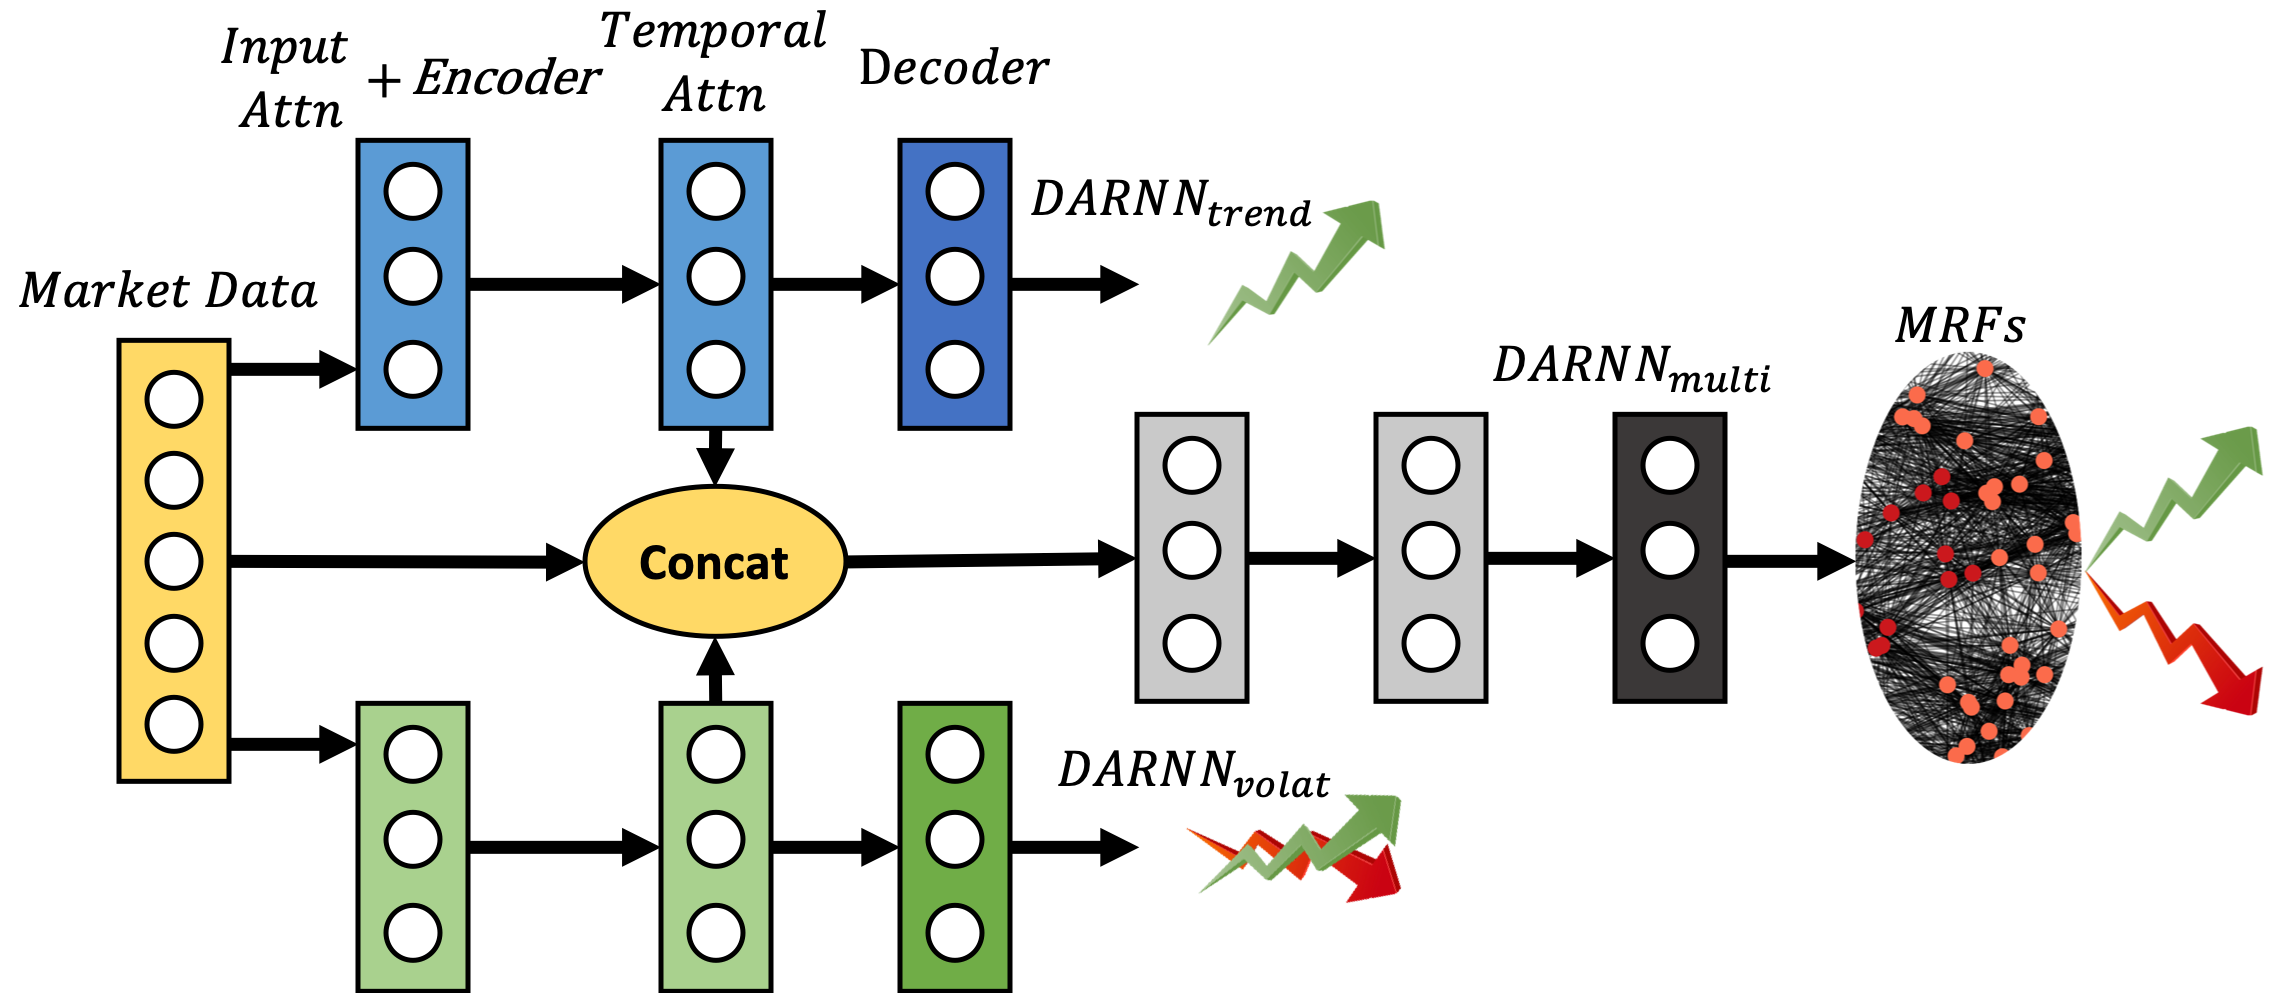
\includegraphics[width=1\columnwidth]{Part2/figures/mmplmrf.png}
  \caption{\label{fig:mrfrnn} Multi-task RNN-MRFs architecture. Note 
  that the output of $\text{DARNN}_{\text{multi}}$ only corresponds to one 
  node's unary feature in MRFs.}
\end{figure}

All three DARNN modules share the same raw market price data.
Here, we denote the time-series dataset as $\mX$ where
$\mX=(\vx_1,\vx_2,\dots,\vx_T)\in \sR^{N\times T}$. We use
$\vx^n=(x_1^n,x_2^n,\dots,x_T^n) \in \sR^T$ to denote a driving
series of $T$ time-steps and $\vx_t=(x_t^1,x_t^2 ,\dots
,x_t^N)\in \sR^N$ to denote a snapshot at time-step $t$ of all
$N$ features.

For both DARNN modules at the low level, the input is $\mX \in \sR^{5\times T}$
which contains $5$ exogenous driving series, \textit{i.e.}, opening price, low
price, high price, volume, amount and $1$ target series $\vy =
(y_1,y_2,\dots,y_T) \in \sR^T$. These two modules
aim to predict target series $y_{t+p}$ in the next $p$ time
steps:

$$\hat{y}_{t+p} = \text{DARNN}(y_1,\dots,y_{t},x_1,\dots,x_t)$$

The target series $\vy_{\text{trend}}$ of
$\text{DARNN}_{\text{trend}}$ is the closing price. The target series
$\vy_{\text{volat}}$ of $\text{DARNN}_{\text{volat}}$ is the
standard deviation of closing price over $M$ constant time-steps.
In our implementation we set $M=10$. We use Mean Squared Error
(MSE) as the loss function to train those two modules separately.

To construct the high level DARNN module, which aims to predict
the price movement, we concatenate context vectors $\vc_T$ from
each of low level DARNN module's encoder and raw market price
matrix as the input. The target series $\vy^{\text{binary}}$ is
constructed by the sign function $y_t^{\text{binary}} =
sign(y_{t+p}-y_t)$ where $y_t$ denotes closing price at time-step
$t$. We use cross-entropy as loss function to train the final
$\text{DARNN}_{\text{multi}}$. Logits (outputs before going
through \emph{softmax}) of $\text{DARNN}_{\text{multi}}$ are then
passed to Intra-clique Predictor as unary features.

In order to train MMPL together with MRFs in an end-to-end
manner, we follow the subgradient method proposed by
\citename{witoonchart2017application}. Since our inner loop
proposed in section~\ref{sec:mrflssvm_learning_algo} is actually
a latent structural SVM. Only gradients of parameters and feature
functions need to be updated. In our framework, outputs of
MMPL (Logits of $\text{DARNN}_{\text{multi}}$) are only used as unary features in MRFs' energy functions,
our back-propagation rules can be defined by taking derivative of the objective function \textit{w.r.t} $\vw^U$  defined in
~\eqref{eq:mrflssvm_object}:

\begin{align}
  \label{eq:der_w}
  \frac{\partial L}{\partial \vw^U} = \psi^U(y)-\psi^U(y^*)
\end{align}

\noindent where $y$ is the ground-truth label and $y^*$ is
inferenced label. $\psi^U$ is unary feature
function described in section~\ref{sec:llep}, here it denotes
logits calculated from $\text{DARNN}_{\text{multi}}$. $\vw^U$ is
unary parameter defined in energy function~\eqref{eq:energyfunction_UPH}.
Equations \eqref{eq:der_w} can be directly plugged
into sub-gradient algorithm proposed in \cite{witoonchart2017application}.
Other configurations stay the same with their algorithm.

\subsection{Intra-clique Predictor}
\label{sec:srp}

In this section, we show how to construct an ``Intra-clique
Predictor" to model lead-lag relationships and address the other
two challenges as mentioned in the introduction. Specifically, we
present a binary Markov Random Fields (MRFs) with weighted lower
linear envelopes as higher order (when the clique contains more
than two nodes) energy functions. Note that the algorithm
proposed here is a general framework for classification tasks.
Besides time series classification, it can also be applied to other tasks such as computer vision.

Pairwise energy function is included only to show our framework
applies to general cases. To our best knowledge, there is no
public available definition of pairwise relationship between
stocks. In our implementation, we use logits from MMPL as unary
function and weighted lower linear envelopes as higher order
function to encode lead-lag relationships. Pairwise features are
excluded.

The detail of the optimization algorithm is summarized in
\algref{alg:learning_app}. As we mentioned in
\appref{sec:train_detail}, although we proposed an end-to-end
subgradient algorithm is section \ref{sec:mmpl}, MRFs updated by
such algorithm take too many iterations to converge. Therefore,
we propose a two-stage training procedure. At first stage, MMPL
and MRFs are trained separately. Therefore, MRFs can take
advantage of the efficient latent structural SVM and converge in
a polynomial number of iterations. After all those models are
converged, we then combine them together to conduct end-to-end
training. Note that the CCCP Inner Loop in
\algref{alg:learning_app} is actually solving standard structural
SVM problem. Therefore, at the second stage, we use subgradient
algorithm proposed in section~\ref{sec:mmpl} to replace the CCCP
Inner Loop. Other settings remain the same.

\section{Dataset and Model Settings}
\label{sec:dataset}

To demonstrate the effectiveness of higher order consistency, we
choose three exclusive and the most famous stock indexes on Chinese
stock market to build our input datasets. Their index codes are:
CSI (China Securities Index) 200, CSI 300 and CSI 500 which
contain 200, 500 and 300 constituent stocks respectively. The CSI
300 index selects most liquid A-share stocks. It aims to reflect
the overall performance of China A-share market. The CSI 200 and
500 indexes aim to reflect the overall performance of mid-to-large
and small-to-mid capital A-shares respectively.

All these indexes are exclusive and are refined on a yearly
basis. In this paper, we use fixed versions on 30-JAN-2015. We
then collect their constituent stocks' minute-level data from
05-JAN-2015 to 29-DEC-2017. On Chinese stock market each trading
day has 4 trading hours. So there are 240 samples (minutes) for
each normally traded stock on each day. Each sample contains 6
features: opening price, high price, low price, closing price,
volume, and amount. \footnote{During this period, there are some
  stocks de-listed (SZ000024, SH600485, SH600832 in CSI 200;
  SZ000693, SZ000748, SZ000982 in CSI 500; SH600485, SH600832,
  SZ000024, SH601299 in CSI 300). Therefore, in total we collect
  197, 497 and 296 stocks during this period respectively.} For
each stock, the first $80\%$ days are used to construct the
training set and the last $20\%$ days are used as test set.
Approximately training set and test set contain $33.6$ million
and $4.2$ million samples, respectively. $49.5\%$ of them are
positive movements, $0.3\%$ of them stay unchanged and $50.2\%$
of them are negative movements. For binary classification task,
we follow \citename{mitchell2001characteristics}'s approach and
label all positive movement samples $1$ and $0$ for the other
samples. More labeling details are described in appendix
\ref{sec:train_detail}.

\begin{table}[H]
\centering
\small
\caption{Technical Indicators Selection}
\begin{tabular}{|c|c|} \hline
  Category&Indicator Name\\ \hline
  Momentum& Awesome Oscillator, Money Flow Index\\ \hline
  Volume& \makecell{Chaikin Money Flow\\ On-balance volume mean}\\ \hline
  Volatility& Bollinger Bands (Upper and Lower Bands)\\ \hline
  Trend& \makecell{Average Directional Movement Index\\Moving Average Convergence Divergence}\\ \hline
\end{tabular}
  \label{tab:ta}
\end{table}
To demonstrate the benefits of multi-task RNN over manually designed
technical indicators, we construct technical
indicators datasets. We select 8 most popular indicators, 2 from each
category~\cite{kirkpatrick2010technical} shown in Table
\ref{tab:ta}. In implementation, we use open source package
\emph{Technical Analysis Library in
  Python\footnote{https://github.com/bukosabino/ta}} to calculate
those indicators and all hyperparameters are using package's
default settings without any prior expert knowledge involved
with. After technical indicators calculation, these 8 new
features are concatenated to above market price dataset (5
features at each minute). So the final input dataset for each
single task model contains 13 features in total. Before feeding
into models, we normalize each stock with \emph{z-score} function
using standard deviation and mean calculated in the training set.

For brevity, we denote market price dataset which only contains
$5$ features as \textbf{Market} and the concatenated $13$
features dataset as \textbf{Indicator}. As discussed in
section~\ref{sec:mmpl}, closing price at time $t$ can be directly
used as regression target for $\text{DARNN}_{\text{trend}}$.
Standard deviation of closing price with a window size of $10$ is
used as regression target for $\text{DARNN}_{\text{volat}}$. The
dimensions of hidden state and cell state are fixed as 32 for
$\text{DARNN}_{\text{trend}}$ as well as
$\text{DARNN}_{\text{volat}}$, and 128 for
$\text{DARNN}_{\text{multi}}$. More training details are
described in appendix \ref{sec:train_detail}.

\section{Results}
\label{sec:res}

In order to demonstrate the effectiveness of our framework, we
compare 3 baseline methods, \textit{i.e.},
LSTM~\cite{hochreiter1997long}, attention based LSTM
Encoder\_Decoder~\cite{attention}, and DARNN~\cite{qin2017dual}
on 3 different Chinese Securities Indexes with and without
technical analysis indicators as inputs. Results are summarized
in Table~\ref{tab:result}. All results are reported over the test
sets. We select four metrics (Accuracy, Precision, Recall and F1
Score) as evaluation metrics to justify the effectiveness of the
proposed approach. They are calculated by collecting all
predicted labels of constituent stocks in each CSI index.

\begin{figure}[t]
  \centering
  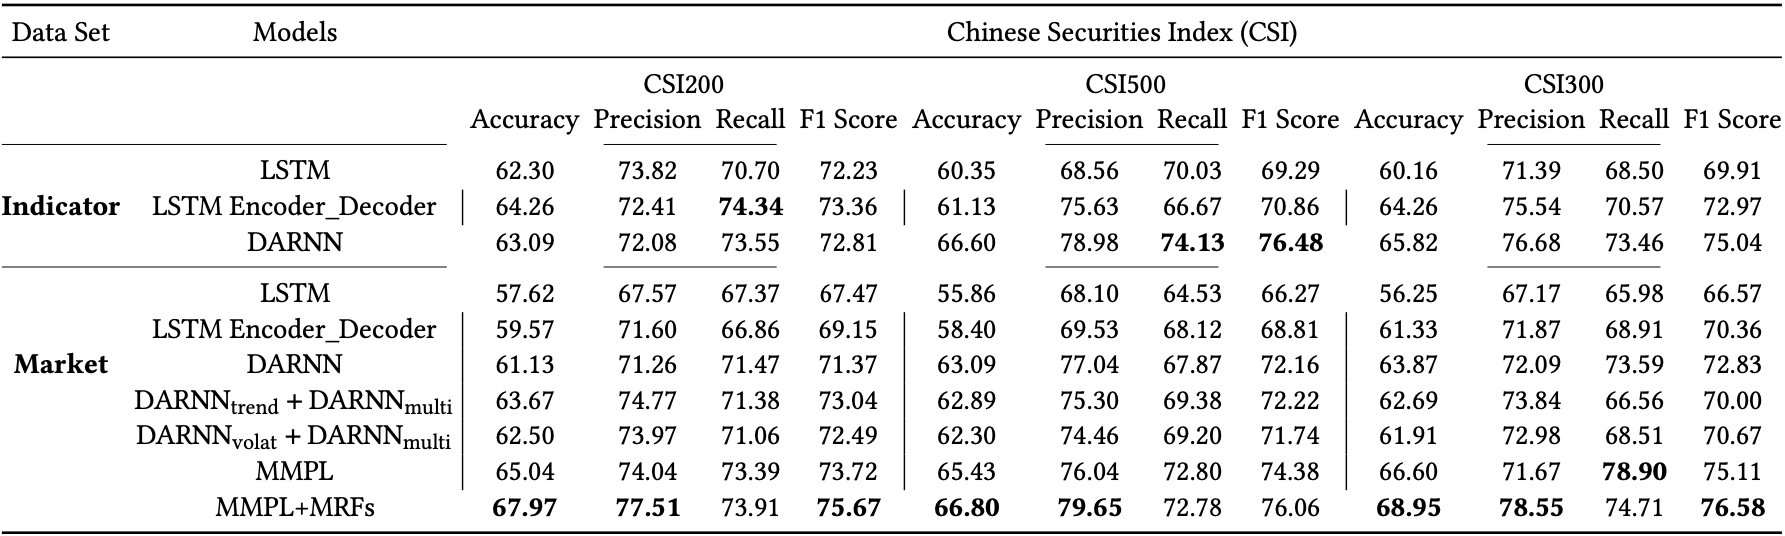
\includegraphics[width=1\columnwidth]{Part2/figures/table_results.png}
  \caption{\label{tab:result} Results: baselines and ablation
    studies. All models have a window size (lag steps) of 20 and
    predict price movement label at the next time step.}
\end{figure}


\subsection{Effectiveness of multi-task framework}

As mentioned earlier, to demonstrate effectiveness of multi-task
framework, we use \textbf{Indicator} dataset, which contains both
market price data and technical analysis indicators as inputs for
baseline approaches and \textbf{Market} dataset which only
contains market price data as inputs for MMPL (multi-task RNN) as
well as baseline methods. For DARNN, we use a hidden size of
$128$. MMPL's configuration is described in
section~\ref{sec:multi_train}. As we can see in
Table~\ref{tab:result}, single task models (LSTM, LSTM
Encoder\_Decoder, DARNN) tested on \textbf{Market} dataset
(without technical analysis indicators as inputs) generally have
worse performance with all 4 metrics. In particular, performance of
DARNN models tested on \textbf{Indicator} dataset is consistently
better than the ones on \textbf{Market} dataset. This proves that
even with hand-crafted features, deep learning models can still
benefit from diversified and complementary features.

To test the effectiveness of multi-task framework, we conduct
ablation study with only one low-level task (\quad
$\text{DARNN}_\text{trend}$ \quad or \\
$\text{DARNN}_\text{volat}$) together with the high-level task
module $\text{DARNN}_\text{multi}$. Results indicate that these
two variants have comparable or slightly worse result than DARNN
on \textbf{Market}. This may because single task model does not
provide diversified features while have more parameters than
DARNN. Finally, MMPL outperforms all single task models and
baseline methods on \textbf{Market}. This suggests that
diversified and complementary tasks can help MMPL extract
effective features. Specifically, by comparing MMPL and DARNN on
\textbf{Market} as well as \textbf{Indicator}, we can see that
MMPL generally outperforms DARNN on CSI200 and CSI300 indexes and
is slightly worse than DARNN on \textbf{Indicator} of CSI500
index. We can conclude that by using multi-task RNNs, we can
extract better or at least comparable features compared with
hand-crafted features.

\subsection{Effectiveness of higher-order MRFs}
In Table~\ref{tab:result}, we can observe that MMPL-MRFs
framework consistently outperforms other baselines on all 3 CSI
index constituent stocks. It shows evidence that higher-order
energy function can help with encoding clique level consistency
thus improving overall prediction performance. One interesting
point to note is that the recall rate of MMPL-MRFs is constantly
lower than other baselines. This can be seen as a trade off
between accuracy and recall rate. However, it is worth to mention
that for stock price movement prediction, high accuracy and
precision are much preferred than recall rate. Another
interesting phenomenon is that MMPL-MRFs gives more improvement
on CSI200 and CSI300 while less improvement over DARNN trained
with technical analysis indicators on CSI500. One possible reason
is that CSI200 and CSI300 select most liquid and representative
stocks in Chinese stock market. Those stocks exhibit much
stronger and higher order consistency than illiquid stocks.
CSI500 selects small-mid capital stocks which are less liquid and
contains much more noisy movements.

In the training stage, our algorithm converges in 4 to 19
CCCP outer loops. The average inference time of graph-cut
algorithm is 34 seconds.

\subsection{Visualization of higher-order consistency}

In order to further investigate higher-order MRFs' effectiveness,
we design a heat-map to visualize CSI300 index intra-clique
higher-order relationship in figure~\ref{fig:consistency}.

\begin{figure*}[t]
  \centering
  \setlength{\tabcolsep}{20pt}
  \begin{tabular}{cc}
  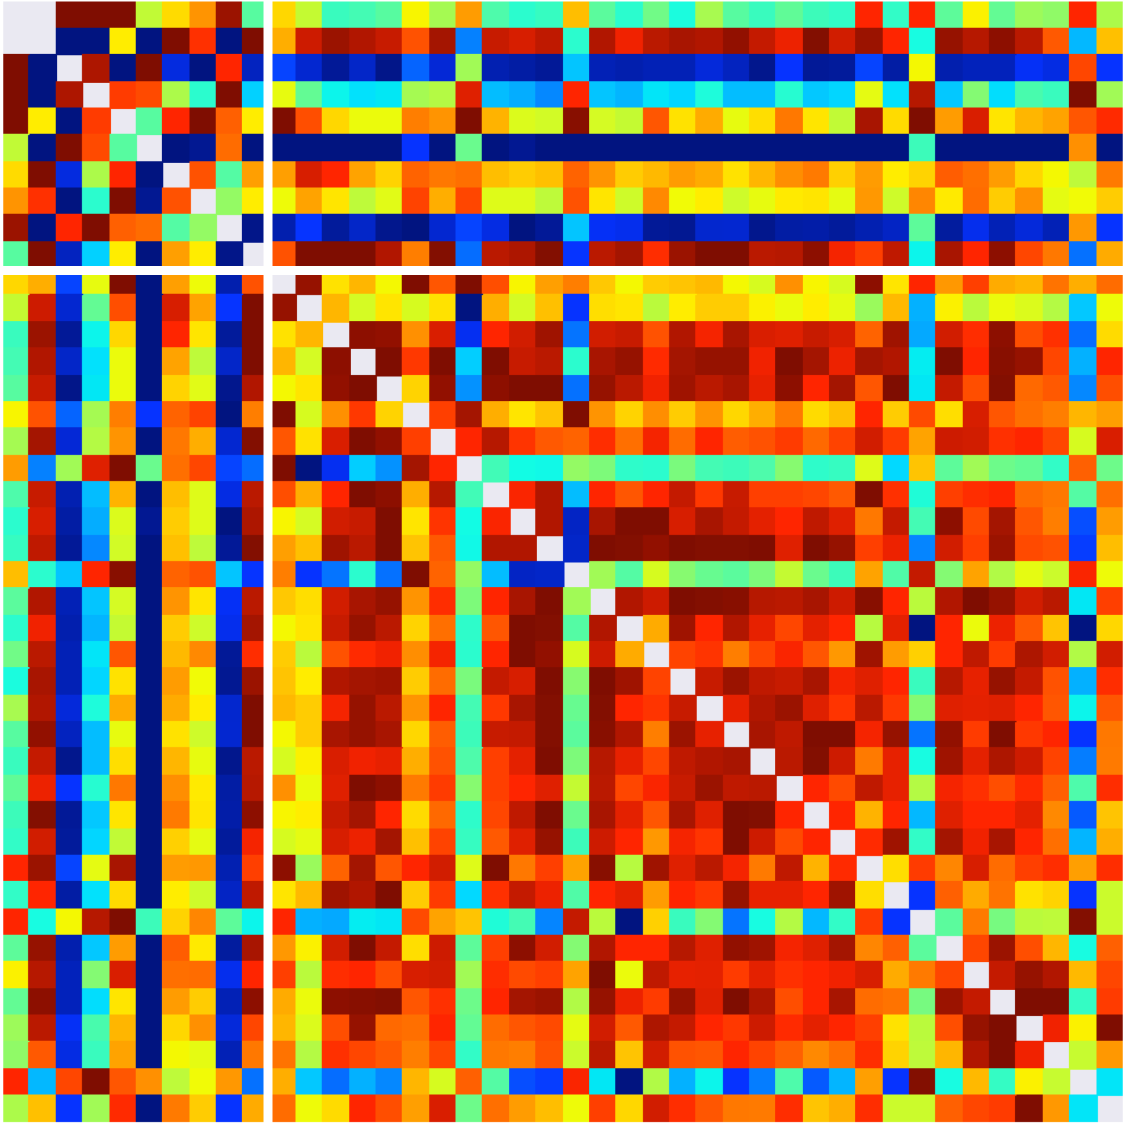
\includegraphics[width=0.4\columnwidth]{Part2/figures/gt.png}&
\includegraphics[width=0.48\columnwidth]{Part2/figures/mmpl.png}\\
{\small (a) Ground-truth} & {\small (b) MMPL }\\
    \includegraphics[width=0.4\columnwidth]{Part2/figures/mrf.png}\\
{\small (c) MMPL-MRFs}\\
  \end{tabular}
  \caption{\label{fig:consistency} Higher order consistency
    visualization. (a) is calculated
    directly from ground truth labels on test set.
    (b)
    is calculated using predicted labels of MMPL without MRFs on the
    test set.
    (c), we use predicted labels of
    MMPL-MRFs on test set as inputs.}
\end{figure*}

We first select two sectors: nonferrous metal sector, which
contains 10 constituent stocks, and infrastructure sector, which
contains 35 constituent stocks from CSI300 index \footnote{These
  two sectors are selected only because painting many sectors in
  one figure would be too messy to interpret and those two
  sectors have appropriate clique size (number of stocks) for
  visualization. Conclusions from these two sectors also apply to
  other sectors}. We then measure consistency level between each
two of these constituent stocks. In order to capture their
temporal relationship, we propose a novel consistency measure
which is calculated on temporal intervals.
% Let $\C\in\{\text{Nonferrous Metal},\text{Infrastructure}\}$
% denotes one clique. $\by_c=\{\by_i \in \C\}$ denotes a set of
% time-series $\by_i^T=\{y_i^1,y_i^2,...,y_i^T\}$ for all stocks

Let $\vy_i^T=\{y_i^1,y_i^2,...,y_i^T\}$ denotes time-series for
stock $i$. $y_i^t\in \{0,1\}$ is the binary price movement label
at time $t$. We segment time-series $\vy_i^T$ into
$N=\lceil\frac{T}{P}\rceil$ non-overlapping intervals
$\{y_i^n,y_i^{n+1},...,y_i^{n+P}\}$ with fixed length $P$. For
any two stocks $i$ and $j$, we calculate the difference
$d_{ij}^n=\sum_n^{n+P}{y_i^n}-\sum_n^{n+P}{y_j^n}$ of how many
times positive price movement happen in the $n$-th time interval
in each stock. Then the consistency level $c_{ij}$ between stocks
$i$ and $j$ can be calculated via a $\ell_1\text{norm}$:
$$c_{ij}=-\|\mathbf{d}_{ij}\|_1$$
\noindent where
$\mathbf{d}_{ij}=\{d_{ij}^1,d_{ij}^2,...,d_{ij}^N\}$. We
normalize $c_{ij}$ into interval $[-1,1]$. Each entry in
figure~\ref{fig:consistency} denotes a consistency level measure
$c_{ij}$. The larger the $c_{ij}$ is, the higher of consistency
level between stock $i$ and stock $j$, the color of corresponding
entry is closer to red, and vice versa. As we mentioned, the average duration of information
arrival-conduction-integration-release process is 4.04 minutes~\cite{fangyan2012}.
Since which stock is leading at each time interval is elusive, we
set $P=9$ when calculating consistency measures.

As we can see in Figure 4(a), there is a significant red square
area, which means ground-truth heat-map shows strong intra-clique
consistency. This is an evidence that higher-order relationships
do exist within clique of stocks. However, in Figure 4(b), the red
square area is fragmented into many little pieces. The whole
area's color is closer to blue when compared to ground-truth
heat-map, which means that MMPL captures little higher-order consistency.
The reason we still can observe a shape of red square
is that the accuracy of MMPL model on CSI300 is $66.6\%$.
However, we can still conclude that the accuracy of single MMPL
model mainly comes from unary features and it fails to capture
higher order consistency of different stocks belonging to the same clique.
On the contrary, even though MMPL-MRFs model's accuracy on CSI300
index is only $2.35\%$ better than MMPL model, we can observe
that heat-map Figure 4(c) is more close to ground-truth heat-map than
heat-map Figure 4(b). There is a much clear red square and the number of
small fragments in red area is also less than Figure 4(b). We can
conclude that MMPL-MRFs models learn to utilize both unary
features from MMPL as well as higher-order relationships encoded
in MRFs.

\section{Conclusions}
\label{sec:conc}

Here we show how to model individual stock price predictions
without hand-crafted features and encode lead-lag relationships
between stocks using weighted higher-order MRFs. A multi-task
neural network framework - Multi-task Market Price Learner (MMPL)
- is proposed to automatically extract diversified and
complementary features from individual stock price sequences.
Features learned by MMPL are passed to a binary MRF with a
weighted lower linear envelope energy function to utilize
intra-clique higher-order consistency between stocks. An
efficient latent structural SVM algorithm is designed to learn
MRFs in polynomial time. Finally, the MRFs and MMPL are trained
end-to-end using the sub-gradient algorithm. Extensive
experiments are conducted on three major Chinese stock market
indexes, and the proposed MMPL-MRFs achieve the best accuracy on
all three indexes.

Our work provides a number of directions for future research. In
this work we proposed a multi-task recurrent neural network for
stock price prediction. While we directly use DARNN as a proof of
concept, other, more dedicated architectures are worthy of
exploration. As well as time series tasks, we can also
investigate how the latent SSVM framework performs on computer
vision tasks. Another interesting direction is to investigate the
implicit relationship between the expert-defined index list and
graph RNN~\cite{you2018graphrnn}, which could further help to
reduce the domain knowledge required by our framework.

%%
%% The acknowledgments section is defined using the "acks" environment
%% (and NOT an unnumbered section). This ensures the proper
%% identification of the section in the article metadata, and the
%% consistent spelling of the heading.

\section{Training Details}
\label{sec:train_detail}

\subsection{Initialization of lower linear envelope}
\label{sec:sup_init}

We assume that the more evenly distributed of $W_c(Y_c)$ where
$c\in\cal C$ on $x$ axis, the more rich representation (number of
linear functions) the energy function should have. In order to
initialize $\vtheta$, we first determine the x-coordinate of
sampled points $sp$. Then we sample its y-coordinate from a
uniform distribution ${\cal U}(\text{upbound},\text{upbound}-0.5)$ to add some
randomness in our initialization as well as maintain concavity.
Linear parameters $a_k$ and $b_k$ are later calculated using
those sampled points $sp_k$ and $sp_{k-1}$. At last we encode
$\{a_k,b_k\}_{k=1}^K$ into $\vtheta$ using
equation~\eqref{eq:llsvm_param}. This algorithm is summarized in
\algref{alg:init_theta}.

\begin{algorithm}[h]
  \begin{algorithmic}[1]
    \STATE{$gap=\frac{1}{K}$, $a_1={\cal U}(0,1e6)$, $b_1=0$,
      $sp_1=(0,0)$, $w_0=0$, $counter=2$} \FOR{each
      clique $c\in \cal C$} \STATE{Compute weighted clique value
      $w_c=W_c(y_C)$} \IF{$w_c-w_{c-1}>gap$}
    \STATE{$upbound = a_{counter}w_c+b_{counter}$\\
      $sp_{counter}=(w_c,{\cal U}(upbound-0.5,upbound))$\\
      Calculate $a_{counter}$ and $b_{counter}$ using
      $sp_{counter-1}$ and $sp_{counter}$\\
      $counter=counter+1$}
    \ENDIF
    \ENDFOR
    \STATE{If $counter<K$, remaining $a$s and $b$s are all set to
      be $a_{counter}$ and $b_{counter}$} \STATE{Calculate
      $\vtheta$ using $\{a_k,b_k\}_{k=1}^K$}
  \end{algorithmic}
  \caption{\label{alg:init_theta} Empirical initialization
    algorithm for $\vtheta$}
\end{algorithm}

\subsection{Multi-task training}
\label{sec:multi_train}

To improve accuracy and reduce over-fitting, we add a drop out
layer between input layer and LSTM layer with a ratio of $0.2$.
We also clip and normalize gradients during back-propagation
stage with a maximum norm of $5.0$ to prevent gradient exploding
issue. As pointed out by \citename{lample2016neural}, the
question of ``when should the training schedule switch from one
task to another task?'' or ``should each task be weighted
equally?'' remains open. In our implementation, we follow the
proportional sampling approach described by
\citename{sogaard2016deep}. After a backward pass completed, we
randomly sample a new task as well as its batch data as the next
task to be trained. In practice, we use a proportion of
$[0.25,0.25,0.5]$ for three tasks respectively. This mechanism
helps multi-task model to avoid \emph{Catastrophic Forgetting}
phenomenon which means lower level model forgets learned
knowledge during higher level model back-propagation pass.

Even though we propose an end-to-end training algorithm for MMPL
and MRFs in section~\ref{sec:mmpl}, MRFs inference stage is still
too slow to be trained jointly with MMPL. To overcome this
difficulty, we implement a two stages training procedure. We
first add a \emph{softmax} layer on top of
$\text{DARNN}_{\text{class}}$ and train MMPL separately from
MRFs. We use \emph{Negative Log-likelihood} as the loss function.
At the second stage, after MMPL converge, we remove the
\emph{softmax} layer and re-train it together with MRFs. One
issue we must mention is that, even though we use binary MRFs
which can only predict positive / negative price movement, we
find there is a significant amount of time when stock price
remains no change. We find it benefits the performance a lot if
we treat the classification as a three classes problem rather
than a binary classification problem during the first stage.
Therefore, at the first stage, the \emph{softmax} layer will
output probability for three labels: \emph{negative movement},
\emph{no changes} and \emph{positive movement}. Since binary MRFs
still needs a two dimension input as part of unary energy
function, after the \emph{softmax} layer is removed, we add an
additional linear mapping layer between logits of MMPL and MRFs
at the second stage.

\subsection{End-to-end multi-task RNN-MRFs training}
\label{sec:mrf_train}

\begin{algorithm}[h]
  \begin{algorithmic}[1]
    \STATE{Set $MaxIter = 100$}
    \STATE{ {\bf input} training set $\{\vy_i\}_{i=1}^{n}$, regularization constant $C > 0$,
      and tolerance $\epsilon \geq 0$}
    \STATE{Initialize $\vtheta$ using \algref{alg:init_theta}}
    \REPEAT \STATE{CCCP Outer Loop}
    \STATE{Set $iter = 0$}
    \FOR{each training example, $i = 1, \ldots, n$}
    \STATE{compute $ \vz_i^*=\argmax_{\mathbf{z} \in \mathcal{Z}}
      \theta \cdot \psi(\mathbf{y}_i,\mathbf{z}) $}
    \ENDFOR

    \STATE{ {\bf initialize} active constraints set ${\cal C}_i = \{ \}$ for all $i$}
    \REPEAT \STATE{CCCP Inner Loop}

    \STATE{solve the quadratic programming problem in
      equation~\ref{eq:mrflssvm_object} with respect to active
      constraints set ${\cal C}_i$ for all $i$ and concavity constraints
      $A\vtheta\geq \epsilon$ to get
      $\hat{\vtheta}$ and $\hat{\vx_i}$}

    \FOR{each training example, $i = 1, \ldots, n$}
    \STATE{compute $\hat{\vy_i},\hat{\vz_i} = \argmin_{\vy}
      E(\vy,\vz; \hat{\vtheta}) - \Delta(\vy, \vz, \vy_i)$}
    \IF{$\hat{\xi}_i + \epsilon \!<\! \Delta(\hat{\vy_i},
      \hat{\vz_i}, \vy_i) -
      E(\hat{\vy_i},\hat{\vz_i}; \hat{\vtheta}) + E(\vy_i, \vz_i^*; \hat{\vtheta})$}
    \STATE{${\cal C}_i \leftarrow {\cal C}_i \cup \{{\vy}_i^\star\}$}
    \ENDIF
    \ENDFOR
    \UNTIL{no more violated constraints}
    \STATE{ {\bf return} parameters $\hat{\vtheta}$}
    \STATE{Set $iter = iter+1$}

    \UNTIL{$iter\geq MaxIter$}
    \STATE{ {\bf return} parameters $\hat{\vtheta}$}
  \end{algorithmic}
  \caption{\label{alg:learning_app} Learning lower linear envelope
    MRFs with latent variables.}
\end{algorithm}

With converged MMPL and MRFs at hand, now we can go forward to
train them in an end-to-end manner. We only include pairwise
energy function through section~\ref{sec:srp} and
section~\ref{sec:opt} to show a general application of our
proposed algorithm. In the case of Chinese stock market, to our
best knowledge there is no public available definition of
pairwise relationship between stocks. Therefore, in our
implementation we only use unary and higher order energy
function. Each stock is then treated as a node in MRFs and each
stocks group which has lead-lag relationships is treated as a
maximum clique in MRFs. One benefit of MRFs clique is that we can
embed domain expert knowledge about industry classification as
maximum cliques into our model. We choose to use Tonghuashun
industry classification \cite{ths} in our model. One subtle but
crucial detail about modeling lead-lag effect lies in
equation~(\ref{eqn:potential2}). Recall that $W_{\!c}(\vy_c) =
\sum_{i \in c} w_i y_i$ with $w^c_i \geq 0$ and $\sum_{i \in c}
w^c_i = 1$ which are weights for stocks in each clique.
Therefore, leading stocks should have a higher weights while
lagging stocks should have lower weights. In our implementation,
we use constituents' weight defined in CSI200, CSI500 and CSI300
as their weights in equation~(\ref{eqn:potential2}) and normalize
them to ensure the summation equals $1$.



%%% Local Variables:
%%% mode: latex
%%% TeX-master: "../thesis"
%%% End:


%% Conclusion
%%
%% Template conclusion.tex
%%

\chapter{Conclusion and Future Work}
\label{cha:conclusion}

We summarize our work in this chapter. We will also conclude its
advantages and disadvantages basing on our synthetic
(section~\ref{sec:synth-check}) and real-world
(section~\ref{sec:foregr-extr}) experiments' results. Our work
also provide some insights to our future work which we will
briefly discuss in this chapter.


\section{Conclusion}
\label{sec:conclusion}

Lower linear envelope binary MRFs are raising interests due to
its capability for encoding higher-order consistency constraints
over large sets of random variables. \citename{gouldlearning} has
shown how to perform exact inference and learning of this problem
under the max margin framework. In order to transform the lower
linear envelope function to a linear combination formulation,
they interpolates it with a set of fixed space sample points.
Thus their algorithm is only able to learn the shape of the lower
linear envelope function approximately.

The main goal of our research is to learn the lower linear
envelope function exactly. Based on their work, we explore a
variant of their formulation by introducing auxiliary variables
back to the energy function to formulate an exact representation.
We find that the lower linear envelope function under the
quadratic pseudo-Boolean formulation~\eqref{eq:originalenergy}
itself is an inner product of parameters and features thus can be
written into a linear combination directly. Under this
formulation the inference algorithm (\emph{st min cut}
construction) developed by \citename{gouldlearning} still adapts
to our problem. Therefore, we are still able to conduct exact
inference on our problem. We developed the learning
\algref{alg:learning} using an extension of the max margin
framework which is known as latent structural SVM. However, this
algorithm is only guaranteed to decrease the objective function
to a local minimum thus the initial point will affect the overall
performance. In order to overcome this issue we also proposed an
empirical initialization \algref{alg:init_theta}.

In order to examine the effectiveness of our new algorithm, we
repeat two experiments \citename{gouldlearning} conducted in
their research and compare both results. In the first synthetic
checkerboard experiment, we found that in general the new
algorithm's accuracy is at least as well as the previous one. But
on harder problem~\ref{sec:unif-distr-squar} the new method
outperforms previous one significantly. The new method is much
more computationally expensive during the training period.
However it is more efficient during the testing stage because of
the simplicity of the shape of the lower linear envelope. We also
found that the shape learned by the new method can shift along
with the changes of the input data which proves that we can learn
the lower linear envelope exactly.

We then take our algorithm to a harder real-world
experiment~\ref{sec:foregr-extr}. It turns out that our new
method has a slightly increasing in overall accuracy (0.6\%)
compared to the previous method. There are much less holes in
images inferred by our new method which certificates the lower
linear envelope function learned by our formulation can better
enforce higher order consistency in large cliques. However, the
performance various significantly between cross-validation folds
which indicates there are some generalization issues existing in
our new method.

At last we summarize the advantages and disadvantages as
following.

\bigskip

Advantages of the new method (compared to the previous
method~\cite{gouldlearning,Gould:ICML2011}):

\begin{itemize}
\item Able to learn the lower linear envelope exactly.
\item Performs better (higher accuracy) on harder problems.
\item Efficient to compute during testing due to the simplicity
  of the shape of the lower linear envelope function.
\end{itemize}

Disadvantages of the new method:

\begin{itemize}
\item Only guaranteed to decrease to the local minimum.
\item Computationally expensive during training.
\item Generalization various significantly.
\end{itemize}




\section{Future Work}
\label{sec:futurework}

As we suggested in the conclusion, our new method seems to have
some generalization issues (figure~\ref{fig:grabcut_worst} for
example). It will be our primal goal to keep investigating into
this problem. We also proposed an empirical initialization method
in section~\ref{sec:mrflssvm_learning_algo}. For future work we
would compare this method to others.

Our research also provide insights to further directions.
Extending our approach to multi-label MRFs seems to be very
promising. Other straightforward extensions include the
introduction of features for modulating the higher-order terms
and the use of dynamic graph cuts~\cite{Kohli:PAMI07} for
accelerating loss-augmented inference within our learning
framework. Other optimization algorithms for solving our learning
problem may also be considered, \eg the subgradient
method~\cite{Nowozin:2011, Bertsekas:2004}.






%%% Local Variables: 
%%% mode: latex
%%% TeX-master: "thesis"
%%% End: 


%%%%%%%%%%%%%%%%%%%%%%%%%%%%%%%%%%%%%%%%%%%%%%%%%%%%%%%%%%%%%%%%%%%%%%
% Here begins the end matter

%%%
%% 
%%

\appendix

\chapter{Some Other Stuff}
\label{app:app1}

\section{Why I Did It}
\label{sec:why3}

\chapter{More Stuff}
\label{app:app2}

%%% Local Variables: 
%%% mode: latex
%%% TeX-master: "thesis"
%%% End: 


\backmatter

%%%%%%%%%%%%%%%%%%%%%%%%%%%%%%%%%%%%%%%%%%%%%%%%%%%%%%%%%%%%%%%%%%%%%%%
%% Other options
% \end{doublepage}

\bibliographystyle{abbrvnat}
\bibliography{Bibs/thesis,Bibs/long,Bibs/scene,Bibs/proposal,Bibs/fin}
\printindex

\end{document}

%%% Local Variables: 
%%% mode: latex
%%% TeX-master: "thesis"
%%% End: 



